\documentclass[aspectratio=169,handout]{beamer}
\usepackage{beamerthemeCOOP}
%packages%
%\usepackage{savesym}
%\usepackage{longtable}
%\usepackage{listings}
%\usepackage{placeins}
%\usepackage[font=itshape,noorphans=true]{quoting}

%font
\usepackage{amsmath,amsfonts,amsthm,amssymb,mathtools,stmaryrd,xpatch}
\usepackage[T1]{fontenc}
\usepackage{libertine}
\usepackage[libertine]{newtxmath}
\usepackage{appendixnumberbeamer}

%\usepackage{array}
%\usepackage{makecell}
%\usepackage{todonotes}
%\usepackage{graphicx}
\usepackage{color}
%\usepackage{emptypage}
%\usepackage[utf8]{inputenc}
%\usepackage[toc,page]{appendix}
%\usepackage{listings}
%\usepackage[per-mode=fraction]{siunitx}
%\usepackage[automark]{scrpage2}
%\usepackage{hyphsubst}
%\usepackage{textpos}
%\usepackage{wrapfig}
%\usepackage[format=plain, skip=5pt, labelfont=bf]{caption}
\usepackage[hang]{subfigure}
%\usepackage[labelfont=normalfont]{subcaption}
\usepackage[english]{babel}
\usepackage{tikz}
%\usetikzlibrary{%
%	calc,trees,positioning,automata,arrows,chains,shapes.geometric,%
%	decorations.pathreplacing,decorations.pathmorphing,shapes,%
%	matrix,shapes.symbols%
%}%
%\let\openbox\undefined
\usepackage[vlined,linesnumbered,resetcount]{algorithm2e}
%\usepackage[ruled,vlined,linesnumbered,resetcount]{algorithm2e}
\usepackage[numbers,sort]{natbib}
%\usepackage{bussproofs}
%\usepackage{stackengine}
\usepackage{enumitem}
\usepackage{framed}
%\usepackage{url}
%\urlstyle{same}
\usepackage[capitalise]{cleveref}
%\usepackage[utf8]{inputenc}
\usepackage{hyperref}

\usepackage{etoolbox}% http://ctan.org/pkg/etoolbox
\usepackage{array}
\AtBeginEnvironment{figure}{\setcounter{subfigure}{0}}

\usepackage{pbox}
\usepackage[export]{adjustbox}

%Meta-Informationen%

%\newcommand{\mylogo}{./hm_logo_alt}
\newcommand{\mydate}{\today}

%\addto\captionsngerman{%
%\renewcommand{\figurename}{Abb.}%
%\renewcommand{\tablename}{Tab.}%
%}
\graphicspath{{pictures/}}
\hypersetup{pdfauthor={Benedikt Sebastian Zönnchen}}
\hypersetup{pdftitle={Efficient parallel algorithms for large-scale pedestrian simulation}}

\newcommand{\shotAbstractEng}{
The understanding and prevention of catastrophes at large-scale events are of utmost societal importance. 
For that, pedestrian simulation has proven to be a potent tool.
Using microscopic pedestrian simulations, researchers and practitioners investigate the mechanisms and preconditions that lead to dangerous situations such as harmful crowd pressures.
Simulations reveal the behaviors and characteristics of human crowds and suggest practical ways to prevent catastrophes.

However, microscopic pedestrian simulations are computationally expensive.
Yet, it is necessary to model each individual to predict crucial phenomena.
Despite their computational cost, real-time simulations are required to make reliable predictions during ongoing events and to enhance a research field that integrates more and more data-driven methods.
To achieve this temporal requirement, we have to introduce and exploit efficient and parallel algorithms.

In this thesis, I follow the call for efficient and scalable simulations by analyzing existing and introducing new parallel algorithms.
I introduce parallelism to a class of microscopic models, i.e., optimal steps models, and show that real-time simulations of half a million participants are possible.
In addition, I develop efficient and parallel algorithms to construct navigation fields: a robust technique to model pedestrian wayfinding.
A new meshing algorithm reduces the problem size and a novel numerical method exploits similarities of consecutively solved eikonal equations.
In combination, real-time dynamic navigation field computation becomes possible for many large-scale scenarios.
}

\newcommand{\shotAbstractGer}{
Katastrophen inmitten von Großveranstaltungen verstehen und verhindern ist von größter ge\-sell\-schaft\-lich\-er Bedeutung.
Für diese Aufgabe haben sich Fußgängersimulationen als wirksames Werkzeug bewährt.
Mit ihrer Hilfe unter\-such\-en Forscher und unmittelbare Anwender die Voraussetzungen und Zusammenhänge, die zu gefährlichen Situationen, wie kritischen Stauungen, führen.
Aus den gewonnenen Erkenntnissen über das Verhalten und der Bewegung von Fußgängern, können wir praktische Maßnahmen ableiten und dadurch Katastrophen verhindern.
%Durch die Erkenntnisse, die wir über das Verhalten großer Menschenmengendie aus Simulationen gewinnen, können wir praktische Maßnehmen entwickelt und Katastrophen verhindern.

Mikroskopische Fußgängersimulationen sind jedoch rechenintensiv.
Um aussagekräftige Vor\-her\-sagen zu erzielen, ist, bis heute, die Modellierung jedes einzelnen Individuums erforderlich.
%um entscheidende Phä\-no\-me\-ne vorherzusagen
Trotz des dadurch entstehenden Rechenaufwands, wird der Ruf nach Echtzeitsimulationen immer lauter.
%Zugleich sind, trotz des entstehenden Rechenaufwands, Echtzeitsimulationen erstrebenswert.
Einerseits sollen sie die Anwender mit Vorhersagen während einer laufenden Veranstaltung unterstützen.
%Einerseits sollen sie, bei gerade lauf\-en\-den Er\-eig\-nis\-sen, zuverlässige Vorhersagen ermöglichen.
Andererseits wür\-den sie ein Forschungsfeld bereichern, welches immer mehr daten\-ge\-trie\-bene Methoden integriert.
Um diese zeitliche Anforderung zu erfüllen, müssen wir effiziente und parallele Algorithmen für die Be\-rech\-nung von Per\-so\-nen\-strömen entwickeln und nutzen.

In dieser Arbeit folge ich dem Ruf nach effizienten und skalierbaren Simulationen, indem ich vorhandene Algorithmen analysiere und neue parallele Algorithmen entwickle.
Zunächst führe ich die Parallelität in die sogenannten Optimal Steps Modelle, eine Klasse mikroskopischer Modelle, ein.
Ich zeige, dass dadurch die Simulation einer halben Million (virtueller) Fuß\-gäng\-er in Echtzeit möglich wird.
Darüber hinaus entwickle ich effiziente und parallele Algorithmen zur Berechnung von Navigationsfeldern.
Diese haben sich in der Vergangenheit als robuste Technik zur Modellierung der Weg\-fin\-dung von Fußgängern etabliert.
Ein neuer Algorithmus zur Netzgenerierung reduziert die Größe des zu berechnenden Problems und eine neuartige numerische Methode nutzt die Ähnlichkeit aufeinanderfolgend gelöster Eikonalgleichungen aus.
In Kombination wird der Einsatz dynamischer Navigationsfelder für Echtzeitsimulationen für viele große Sze\-na\-rien ermöglicht.
}

\newcommand{\shotAbstractEngB}{
In an ever more connected world, large-scale events with millions of participants are culturally significant and offer joy, happiness, and a place where the human spirit can grow. 
It is sholcing when things go wrong, and joy turns into harm – when our belonging for connection destroys them forever.
We must learn from accidents of the past, find their causes, and develop mechanisms to prevent them in the future.
Therefore, we study human behavior supported by microscopic pedestrian simulation.
Today, real-time simulations are required to predict the future of an ongoing event and to enhance a research field that integrates more and more data-driven methods.
However, simulations are computationally expensive, and the only way to achieve scalability is parallelization.

In this thesis, I follow the call for efficient and scalable simulations by analyzing existing and introducing new parallel algorithms.
I introduce parallelism to a class of microscopic models, \ie{}, \OSMs{} and show that real-time simulations of half a million participants is possible.
In addition, I develop efficient and parallel algorithms to construct navigation fields -- a robust technique to model the wayfinding of pedestrians.
A new meshing algorithms reduces the problem size and a noval numerical method exploits similarities of consecutive solved eikonal equations.
In combination real-time dynamic navigation field computation becomes possible for many large-scale scenarios.
}

\newcommand{\shotAbstractGerB}{
In einer immer kleiner werdenden Welt, sind Großveranstaltungen mit Millionen von Teilnehmern ein wichtiges kulturelles Gut.
Sie sind eine Quelle des Glück, der Freude und bieten einen Platz an dem der menschliche Geist wachsen kann.
Umso schrecklicher ist es anzusehen, wenn diese Freude in Schaden mündet und unsere Verlangen noch Verbundenheit diese für immer zerstört.
Wir müssen aus vergangenen Fehlern lernen, ihren Ursprung ergründen und zukünftige Unfälle durch präventive Maßnahmen verhindern.
Deshalb studieren wir mittels mikroskopischer Personenstromsimulationen menschliches Verhalten.
Heute benötigen wir Echtzeitsimulationen um die Entwicklung einer anhaltenden Großveranstaltung vorherzusagen.
Zudem helfen uns effiziente Simulationen die aufkommenden datengetriebenen Methoden in unseren Forschungsbereich zu integrieren.
Doch sind mikroskopische Simulationen rechenintensiv und um Skalierbarkeit zu erzielen braucht es Parallelität.

In dieser Arbeit folge ich dem Ruf nach effizienten und skalierbaren Simulationen.
Hierzu analysiere ich existierende Algorithmen und stelle neue parallele Algorithmen vor.
Ich parallelisiere eine ganze Klasse von Personenstrommodellen, nämlich die sogenannten Optimal Steps Modelle.
Ich zeige, dass die Simulation von einer halben Millionen Teilnehmern in Echtzeit möglich ist.
Zusätzlich entwickle ich effiziente und parallele Algorithmen zur Konstruktion von Navigationsfeldern.
Sie sind eine robuste Technik um die Wegfindung von Fußgängern zu modellieren. 
Ein neuer Algorithmus zur Gittererzeugung reduziert die zu lösende Problemgröße und eine neue numerische Methode nutzt Ähnlichkeiten in den aufeinanderfolgend zu lösenden Eikonalgleichungen.
In Kombination werden Echtzeitberechnungen von dynamischen Navigationsfeldern für viele großskalige Simulationsszenarien ermöglicht.
}

\newcommand{\longAbstractEng}{
The understanding and prevention of catastrophes at large-scale events are of utmost societal importance. 
For that, pedestrian simulation has proven to be a potent tool.
Using microscopic pedestrian simulations, researchers and practitioners investigate the mechanisms and preconditions that lead to dangerous situations such as harmful crowd pressures.
Simulations reveal the behaviors and characteristics of human crowds and suggest practical ways to prevent catastrophes.

However, microscopic pedestrian simulations are computationally expensive.
Yet, it is necessary to model each individual to predict crucial phenomena.
Despite their computational cost, real-time simulations are required to make reliable predictions during ongoing events and to enhance a research field that integrates more and more data-driven methods.
To achieve this temporal requirement, we have to introduce and exploit parallelism efficiently.

In this thesis, I follow the call for efficient and scalable simulations by analyzing existing and introducing new parallel algorithms.
At first, I give an overview of microscopic models and navigation fields -- a common technique many models employ.
I identify \OSMs{} to be especially important since their foundation is motivated by social psychology and biomechanics.
I then discuss the relation between parallelism and the behavior of individuals within a large crowd.
Instead of enforcing parallelism by compromising the models, I exploit its natural occurrence.
My \textsc{ParallelEventDrivenUpdate} introduces parallelism into \OSMs{} without changing their definition.
I analyze and use the parallelism defined by the models and show that we can simulate up to half a million agents in real-time on affordable off-the-shelf graphics processing units (GPUs).
In the last part of my thesis, I focus on efficient navigation field computation.
In other words, I focus on efficient methods to solve (multiple) eikonal equations.
Navigation fields realize robust wayfinding to facilitate simulations with complex and large geometries.
First, I enter the area of computational geometry and consider different space discretizations.
I then develop \eikmesh{}, a new meshing algorithm for high-quality unstructured two-dimensional unstructured triangular meshes.
The size of the underlying mesh directly influences the time complexity of numerical solvers.
Therefore, \eikmesh{} constructs a mesh with a localized resolution.
Besides reducing the problem size, I develop the \textsc{InformedFastIterativeMethod}, a novel numerical method that exploits consecutive solved eikonal equations.
It is suitable to efficiently compute dynamic navigation fields and might be the source of new numerical methods to solve the eikonal equation in general.
%
%I introduce parallelism to a class of microscopic models, \ie{}, \OSMs{} and show that real-time simulations of half a million participants is possible.
%In addition, I develop efficient and parallel algorithms to construct navigation fields -- a robust technique to model the wayfinding of pedestrians.
%A new meshing algorithms reduces the problem size and a noval numerical method exploits similarities of consecutive solved eikonal equations.
%In combination real-time dynamic navigation field computation becomes possible for many large-scale scenarios.
}

\newcommand{\longAbstractEngB}{
Human beings are social creatures longing for deep emotional connections.
%We find expressions of this basic human need across different cultures.
Today, large-scale events with millions of participantsa are a manifestation of this desire.
In an ever more connected world, they are culturally significant and offer joy, happiness, and a place where the human spirit can grow. 
It is crushing when things go wrong, and joy turns into harm – when our belonging for connection destroys them forever.
We must learn from accidents of the past, find their cause, and develop mechanisms to prevent them in the future.
Therefore, we study the behavior of humans, their decision-making, and motion.
Computer simulations are an essential part of this effort.
They enable researchers and practitioners to analyze, plan, and manage large-scale events.

Microscopic pedestrian simulations are computationally expensive, but it is necessary to model each individual to observe crucial phenomena. 
Today, real-time simulations are required to predict the future of an ongoing event and to enhance a research field that integrates more and more data-driven methods.
In this thesis, I follow this call by analyzing existing and introducing new efficient parallel algorithms to enable large-scale microscopic pedestrian simulations.

At first, I give an overview of microscopic models and a critical technique they are based on, that is, navigation fields.
I identify \OSMs{} to be especially important since their foundation is motivated by social psychology and biomechanics.
I then discuss the relation between parallelism and the behavior of individuals within a large crowd.
Instead of enforcing parallelism by compromising the models, I exploit its natural occurrence.
My \textsc{ParallelEventDrivenUpdate} introduces parallelism into \OSMs{} without changing their definition.
I analyze and use the parallelism defined by the models and show that we can simulate up to half a million agents in real-time on affordable off-the-shelf graphics processing units (GPUs).
In the last part of my thesis, I focus on efficient navigation field computation.
In other words, I focus on efficient methods to solve (multiple) eikonal equations.
Navigation fields realize robust wayfinding to facilitate simulations with complex and large geometries.
First, I enter the area of computational geometry and consider different space discretization.
I then develop \eikmesh{}, a new meshing algorithm for high-quality unstructured $2$-d unstructured triangular meshes.
The size of the underlying mesh directly influences the time complexity of numerical solvers.
Therefore, \eikmesh{} constructs a mesh with a localized resolution.
Besides reducing the problem size, I develop \textsc{InformedFastIterativeMethod}, a novel numerical method that exploits consecutive solved eikonal equations.
It is suitable to efficiently compute dynamic navigation fields and might be the source of new numerical methods to solve the eikonal equation in general.
}

\newcommand{\longAbstractGer}{
Als soziale Wesen streben wir Menschen nach tief emotionalen Verbindungen.
%Ausdrücke dieses Grundbedürfnisses finden sich in verschiedenen Kulturen.
Heute manifestiert sich dieses Verlangen durch Großveranstaltungen mit Millionen von Teilnehmern.
In einer immer kleiner werdenden Welt, sind Sie ein kulturelles Gut und eine Quelle des Glück, der Freude und ein Platz an dem der menschliche Geist wachsen kann.
Umso schrecklicher ist es, wenn diese Freude in Schaden mündet und unsere Verlangen noch Verbundenheit diese für immer zerstört.
Wir müssen aus vergangenen Fehlern lernen, ihren Ursprung ergründen und zukünftige Unfälle durch präventive Maßnahmen verhindern.
Deshalb studieren wir mittels mikroskopischer Personenstromsimulationen menschliches Verhalten.
Sie ermöglichen es Forschern und Anwendern aus der Praxis Großveranstaltungen zu analysieren, zu planen und besser zu lenken. 

Mikroskopische Personenstromsimulationen sind rechenintensiv, doch ist die Mo\-del\-lier\-ung von einzelnen Individuen notwendig um kritische Phenomene beobachten zu können.
Heute benötigen wir Echtzeitsimulationen, um die Zukunft ablaufender Großveranstaltungen vorherzusagen und die aufkommenden datengetriebene Methoden für uns nutzbar zu machen.
In dieser Arbeit folge ich diesem Ruf.
Ich analysiere existierende und entwickle neuer effizienter paralleler Algorithmen die großskalige Echzeitsimulationen ermöglichen.

Zunächst gebe ich einen Überblick über mikroskopische Personenstrommodelle sowie die Modellierung der Wegfindung durch Navigationsfelder.
Da Optimal Steps Modelle sich auf Erkenntnissen aus der Psychologie und der Biomechanik gründen, identifiziere ich sie als besonders wichtig.
Ich diskutiere den Zusammenhang zwischen Parallelität und dem Verhalten der Individuen innerhalb großer Menschenmengen.
Anstatt Parallelität durch Kompromittierung der Modelle zu erzwingen, nutze dessen natürliches Vorkommen.
\textsc{ParallelEventDrivenUpdate} parallelisiert Optimal Steps Modelle ohne dabei Änderungen an den Modellen vorzunehmen.
Ich analysiere und nutze die Parallelität des bestehenden Modells und zeige dass Echzeitsimulationen mit bis zu einer halben Millionen Agenten auf gängigen Grafikkarten möglich sind.
Im letzten Teil meiner Arbeit, konzentriere ich mich auf die effiziente Berechnung der Navigationsfelder.
In anderen Worten, ich konzentriere mich auf effiziente Methoden um (mehrere) Eikonalgleichungen zu lösen.
Navigationsfelder realisieren eine robuste Wegfindung um Simulationen in einer geometrisch komplexen Umgebung zu ermöglichen.
Zu allererst betrete ich den Bereich der algorithmischen Geometrie und betrachte unterschiedliche Raumdiskretisierungen.
Danach entwickle ich \eikmesh{}, einen neuen Gittergenerierungsalgorithmus für qualititiv hochwertige unstrukturierte zweidimensionale Dreieckgitter.
Da die Gittergröße sich direkt auf die Laufzeit numerischer Verfahren auswirkt, konstruiert \eikmesh{} ein Gitter mit lokalisierter Gitterauflösung.
Neben der Reduzierung der Problemgröße nutzt \textsc{InformedFastIterativeMethod} die Ähnlichkeit der aufeinanderfolgend zu lösenden Eikonalgleichungen ausnutzt. Dieses neue Verfahren eignet sich zur effizienten Berechnung dynamischer Navigationsfelder und ist möglicherweise die Quelle weiterer numerischer Methoden zur Lösung der Eikonalgleichung.
}
%\tikzstyle{every node}=[circle, draw, fill=black!50, inner sep=0pt, minimum width=4pt].palenta@tum.de
%bib spacing
% Commands %
\SetKwRepeat{Do}{do}{while}
\SetKwRepeat{Dou}{do}{until}
\newcommand{\etal}{\mbox{et\,al.\ }}
\newcommand{\ua}{\mbox{u.\,a.\ }}
\newcommand{\zB}{\mbox{z.\,B.\ }}
\newcommand{\dahe}{\mbox{d.\,h.\ }}
\newcommand{\Vgl}{Vgl.\ }
\newcommand{\bzw}{bzw.\ }
\newcommand{\evtl}{evtl.\ }
\newcommand{\HRule}{\rule{\linewidth}{0.5mm}}
\newcommand{\eg}{e.\,g.}
\newcommand{\ie}{i.\,e.}
\newcommand{\mywlog}{w.\,l.\,o.\,g.\ }
\newcommand{\myWlog}{W.\,l.\,o.\,g.\ }

\newcommand{\OpenMP}{Open Multi-Processing}
\newcommand{\FLAME}{Flexible Large-scale Agent Modeling Environment}
\newcommand{\MPI}{Message Passing Interface}
\newcommand{\CA}{cellular automaton}
\newcommand{\CCAs}{Cellular automata}
\newcommand{\CAs}{cellular automata}
\newcommand{\CN}{cellular network}
\newcommand{\OSM}{Optimal Steps Model}
\newcommand{\OSm}{optimal steps model}
\newcommand{\OSMs}{optimal steps models}
\newcommand{\COSMs}{Optimal steps models}
\newcommand{\SFM}{Social Force Model}
\newcommand{\SFMs}{social force models}
\newcommand{\sfm}{social force model}
\newcommand{\CFM}{Centrifugal Force Model}
\newcommand{\GCFM}{Generalized Centrifugal Force Model}
\newcommand{\GNM}{Gradient Navigation Model}
\newcommand{\SDM}{Social Dinstance Model}
\newcommand{\BHM}{Behavioral Heuristics Model}
\newcommand{\ORCAM}{Optimal Reciprocal Collision Avoidance Model}
\newcommand{\NelderAndMead}{\textsc{NelderAndMead}}
\newcommand{\sourceCode}{Source Code}

\newcommand{\domain}{\Omega}
\newcommand{\domainBoundary}{\partial \Omega}
\newcommand{\obstacles}{\mathcal{W}}
\newcommand{\BigO}{\mathcal{O}}
\newcommand{\dObs}{d_\obstacles}
\newcommand{\dDomain}{d_\domain}
\newcommand{\hDomain}{h_\domain}
\newcommand{\polygons}{\mathcal{P}}
\newcommand{\polygon}{p}
\newcommand{\eikmesh}{\textsc{Eik\-Mesh}}
\newcommand{\distmesh}{\textsc{Dist\-Mesh}}
\newcommand{\ruppert}{\textsc{Ruppert}}
\newcommand{\ttriangle}{\textsc{Triangle}}
\newcommand{\V}{\mathcal{V}}
\newcommand{\E}{\mathcal{E}}
\newcommand{\PSLG}{\mathcal{P}}
\newcommand{\myCircle}{\mathcal{C}}
\newcommand{\simplex}{\tau}
\newcommand{\mesh}{\mathcal{T}}
\newcommand{\quality}{\rho}
\newcommand{\abs}[1]{\left| #1 \right|}
\newcommand{\maxAngle}{\theta_{\infty}}
\newcommand{\minAngle}{\theta_{0}}
\newcommand{\radIn}{r_{\text{in}}}
\newcommand{\radOut}{r_{\text{out}}}
\newcommand{\perimeter}{p}
\newcommand{\distmeshFext}{F_{\text{ext}}}
\newcommand{\distmeshFint}{F_{\text{int}}}
\newcommand{\distmeshF}{F}
\newcommand{\scalarProduct}{\cdot}
\newcommand{\GMMGroup}{G}
\newcommand{\eikonalApp}{\phi}
\newcommand{\eikonal}{\Phi}
\newcommand{\eikonalDir}{u}
\newcommand{\eikonalDirVec}{\mathbf{u}}
\newcommand{\eikonalGrid}{v}
\newcommand{\eikonalGridVec}{\mathbf{v}}
\newcommand{\skeleton}{S}
\newcommand{\eikmeshSlidePointMapping}{\ell}
\newcommand{\DT}{\mathcal{DT}}
\newcommand{\FMM}{\textsc{FastMarchingMethod}}
\newcommand{\distmeshf}{\eta}
\newcommand{\distmeshScaleConstant}{\omega}
\newcommand{\distmeshScaleFunction}{\psi}
\newcommand{\distmeshEdgeRatio}{\lambda}
\newcommand{\proofsketch}{\normalcolor\bfseries \color{proofcolor} Proof (sketch).}
\newcommand{\hl}[1]{\textit{#1}}
\newcommand{\gr}[1]{ {\color{mygray}#1} }
\newcommand{\filename}[1]{{\small \texttt{#1}}}
\newcommand{\code}[1]{{\footnotesize\ttfamily #1}}
\newcommand{\myremark}[1]{{\textbf{\color{myred}#1}}}
\newcommand{\osmUtility}{u}
\newcommand{\osmStepLengthDist}{\mu}
\newcommand{\osmStepLength}{r}
\newcommand{\osmPositions}{P}
\newcommand{\osmDestination}{\Gamma}
\newcommand{\peds}{\mathcal{A}}
\newcommand{\xx}{\mathbf{x}}
\newcommand{\yy}{\mathbf{y}}
\newcommand{\vvv}{\mathbf{v}}
\newcommand{\cc}{\mathbf{c}}
\newcommand{\qq}{\mathbf{q}}
\newcommand{\aaa}{\mathbf{a}}
\newcommand{\bb}{\mathbf{b}}
\newcommand{\pp}{\mathbf{p}}
\newcommand{\nn}{\mathbf{n}}
\newcommand{\uu}{\mathbf{u}}
\newcommand{\ee}{\mathbf{e}}
\newcommand{\surface}{\mathcal{S}}
\newcommand{\meanCurvature}{H}
\newcommand{\meanCurvatureApp}{\widetilde{H}}
\newcommand{\plane}{\Pi}
\newcommand{\heat}{q}
\newcommand{\order}{\pi}
\newcommand{\definigRelation}{\pi}
\newcommand{\vertexToLevelIndex}{\chi}
\newcommand{\G}{\mathcal{G}}
\newcommand{\dependencyGraph}{\mathcal{G}}
\newcommand{\curvature}{\kappa}
\newcommand{\curvatureApp}{\widetilde{\curvature}}
\newcommand{\graphCompare}{D}
\newcommand{\updates}{u}
\newcommand{\queue}{\mathcal{Q}}
\newcommand{\lineSegments}{\mathcal{L}}
\newcommand*{\eventset}{E}
\newcommand*{\cellnumber}{n_c}
\newcommand*{\pedsnumber}{n_{\peds}}
\newcommand*{\pedsinrage}{n}
\newcommand*{\cellwidth}{w_{c}}
\newcommand*{\cellheight}{h_{c}}
\newcommand*{\domainwidth}{w_{\domain}}
\newcommand*{\domainheight}{h_{\domain}}
\newcommand*{\pedspeed}{v}
\newcommand*{\cellsize}{\delta_c}
\newcommand*{\pedmaxstep}{\gamma}
\newcommand*{\pedutilitywidth}{\delta_w}
\newcommand*{\myarray}[1]{\mathbf{#1}}
\newcommand*{\pedidarray}{\myarray{I}}
\newcommand*{\cellstartarray}{\myarray{C}_{\text{start}}}
\newcommand*{\cellendarray}{\myarray{C}_{\text{end}}}
\newcommand*{\cellarray}{\myarray{C}}
\newcommand*{\possiblepositionarray}{\myarray{X}}
\newcommand*{\eventarray}{\myarray{E}}
\newcommand*{\positionarray}{\myarray{P}}
\newcommand*{\utilityarray}{\myarray{U}}
\newcommand*{\cellpednumber}{n_{\peds,c}}
\newcommand*{\torsoradius}{\delta_{\text{tor}}}
\newcommand{\probability}{\mathbf{Pr}}
\newcommand{\expect}{\mathbf{Ex}}
\newcommand{\rout}{r_\text{out}}
\newcommand{\rin}{r_\text{in}}
\newcommand{\myscale}{0.6}
\newcommand{\mylemma}{Lemma}
\newcommand{\sect}{section}
\newcommand{\csect}{Section}
\newcommand{\chapt}{Chapter}
\newcommand*{\events}{E}
\newcommand*{\eventnumber}{n}
\newcommand*{\roundnumber}{k}
\newcommand*{\roundindex}{j}
\newcommand{\distanceToObs}{d_\domain}

\DeclareMathOperator{\sign}{sign}
\DeclarePairedDelimiter\ceil{\lceil}{\rceil}
\DeclarePairedDelimiter\floor{\lfloor}{\rfloor}
\DeclareMathOperator{\val}{val}
\DeclareMathOperator{\len}{len}
\DeclareMathOperator{\rhs}{rhs}
\DeclareMathOperator{\lhs}{lhs}
\DeclareMathOperator{\arity}{rank}
\DeclareMathOperator{\nt}{nt}
\DeclareMathOperator{\tpaths}{paths}
\DeclareMathOperator{\tpathscl}{paths-cl}
\DeclareMathOperator{\modulo}{\,\%\,}
\DeclareMathOperator{\scount}{count}
\DeclareMathOperator{\first}{first}
\DeclareMathOperator{\last}{last}
\DeclareMathOperator{\occ}{occ}
\DeclareMathOperator{\lcp}{lcp}
\DeclareMathOperator{\lcs}{lcs}
\DeclareMathOperator{\w}{w}
\DeclareMathOperator{\tree}{tree}
\DeclareMathOperator{\concat}{concat}
\DeclareMathOperator{\ppath}{path}
\DeclareMathOperator{\pos}{\mathcal{P}\textit{os}}
\DeclareMathOperator{\lin}{lin}
\DeclareMathOperator{\myalph}{alph}
\DeclareMathOperator{\out}{out}
\DeclareMathOperator{\act}{act}
\DeclareMathOperator{\ssy}{ssy}
%\DeclareMathOperator{\events}{\mathcal{A}\textit{ct}}
\DeclareMathOperator{\nod}{\mathcal{N}\textit{od}}
\DeclareMathOperator{\run}{\tau}
\DeclareMathOperator{\myprec}{prec}
\DeclareMathOperator{\dom}{dom}
\DeclareMathOperator{\coreach}{\mathcal{C}\textit{o}}
\DeclareMathOperator{\ecl}{\epsilon-cl}
\DeclareMathOperator{\shift}{shift}
\DeclareMathOperator{\mymod}{mod}
\DeclareMathOperator{\myaff}{aff}
\DeclareMathOperator{\mycon}{con}
\DeclareMathOperator{\mysing}{sign}
\DeclareMathOperator{\lfs}{lfs}
\DeclareMathOperator{\Abs}{abs}
\DeclareMathOperator*{\argmax}{arg\,max}
\DeclareMathOperator*{\argmin}{arg\,min}
\usepackage{graphicx}

\definecolor{midnightblue}{RGB}{10,10,44}
\definecolor{navyblue}{RGB}{0,0,120}
\definecolor{crimson}{RGB}{220,20,60}
\definecolor{mydarkgray}{RGB}{33,33,33}
\definecolor{myalgColor}{RGB}{99,99,99}
\definecolor{mygreen}{RGB}{85,168,104}
\definecolor{myorange}{RGB}{221,132,82}
\definecolor{myblue2}{rgb}{0.12156862745098039, 0.4666666666666667, 0.7058823529411765}
\definecolor{myblue3}{rgb}{0.2980392156862745, 0.4470588235294118, 0.6901960784313725}
\definecolor{myblue4}{rgb}{0.2823529411764706, 0.47058823529411764, 0.8156862745098039}
\definecolor{mybluebright}{rgb}{0.00784313725490196, 0.24313725490196078, 1.0}
\definecolor{myred}{RGB}{196,78,82}
\definecolor{mydarkgray}{RGB}{90,90,90}
\definecolor{mygray}{RGB}{179,179,179}
\definecolor{myviolet}{RGB}{129,114,178}
\definecolor{myblue}{RGB}{76,114,202}
\xdefinecolor{mybg}{rgb}{0.7419607843137255, 0.9027297193387159, 0.868958093041138}
\xdefinecolor{myRed}{rgb}{0.7686274509803922, 0.3058823529411765, 0.3215686274509804}
\xdefinecolor{prevColor}{rgb}{0.39215686274509803, 0.7098039215686275, 0.803921568627451}
\xdefinecolor{hmred}{RGB}{228, 24, 58}
\xdefinecolor{mylightblue}{rgb}{0.8584083044982699, 0.9134486735870818, 0.9645674740484429}

\definecolor{mybrightblue}{rgb}{0.00784313725490196, 0.24313725490196078, 1.0}
\definecolor{mybrightred}{rgb}{0.9098039215686274, 0.0, 0.043137254901960784}

\xdefinecolor{myalgColor}{rgb}{0.7686274509803922, 0.3058823529411765, 0.3215686274509804}

%%% Title page %%%
%\defbeamertemplate*{title page}{customized}[1][]
%{
%	\usebeamerfont{title}\inserttitle\par
%	\usebeamerfont{subtitle}\usebeamercolor[fg]{subtitle}\insertsubtitle\par
%	\bigskip
%	\usebeamerfont{author}\insertauthor\par
%	\usebeamerfont{institute}\insertinstitute\par
%	\usebeamerfont{date}\insertdate\par
%	\usebeamercolor[fg]{titlegraphic}\inserttitlegraphic
%}
\title{{\huge The Fast Marching Method}}
%\subtitle{\vspace{0.25cm}\large Die \textsc{FastMarchingMethod}\vspace{-0.25cm}}
\author{\href{mailto:zoennchen.benedikt@hm.edu}{Dr. Benedikt Zönnchen}} 
\date{11. Juni 2024}
\institute{\vspace{0.25cm}%
	\Large%
	%Hochschule München\\ \vspace{5mm}%
	
\includegraphics[height=20pt]{./figs/logo/Hochschule_Muenchen_Logo}}
%%% End Title page %%%
\setbeamercovered{transparent}

\begin{document}
\begin{frame}[plain]
 \titlepage
\end{frame}

\begin{frame}
	\frametitle{Outline}
	\tableofcontents
\end{frame}

\section{Defining the Problem}
\begin{frame}
	\frametitle{Defining the Problem}
	\begin{figure}
		\centering
		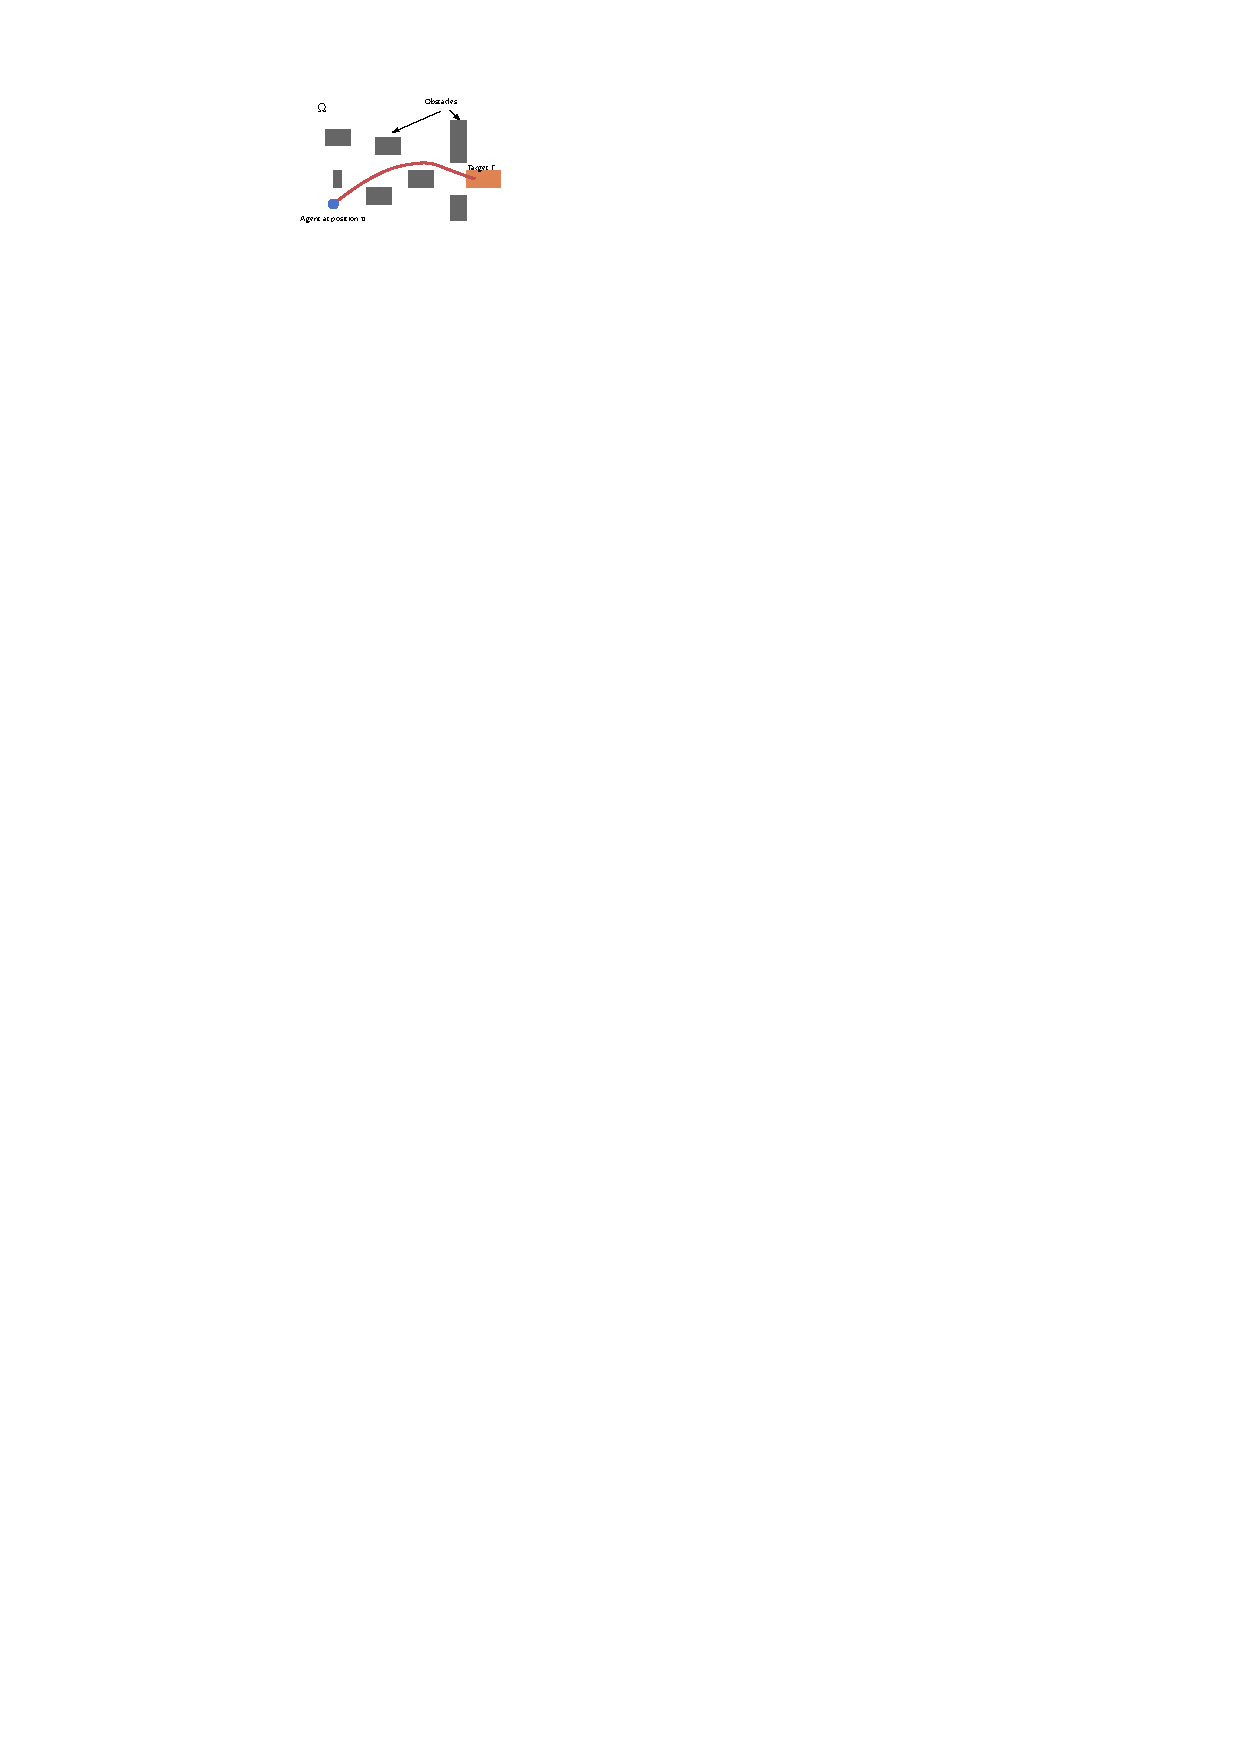
\includegraphics[width=0.6\textwidth]{./figs/wayfinding_en.pdf}
	\end{figure}
\end{frame}

%ODO: plot different d_Gamma
\begin{frame}
	\frametitle{Defining the Problem}
	What we are looking for is a \textbf{distance function} 
	
	$$d_{\osmDestination}: \mathbb{R}^2 \rightarrow \mathbb{R}$$
	
	that gives us the distance to our target region $\osmDestination$ for any position $\uu$  in our spatial domain $\domain$.\\
	\vspace{1cm}
	The gradient of this distance functions $-\nabla d_{\osmDestination}$ gives us the direction in which we or the agent should move.
\end{frame}

\begin{frame}
	\frametitle{Defining the Problem}
	If there is no obstacle ``in the way'', then an appropriate distance function is the Euclidean distance
	
	$$d_{\osmDestination}(\uu) = \min_{\vvv \in \osmDestination} \Vert \uu - \vvv\Vert$$
	
	 and the \textbf{shortest path} from $\osmDestination$ to $\uu$ follows the gradient $-\nabla d_{\osmDestination}$:
	\begin{figure}
		\subfigure[Follow $-\nabla d_{\osmDestination}$]{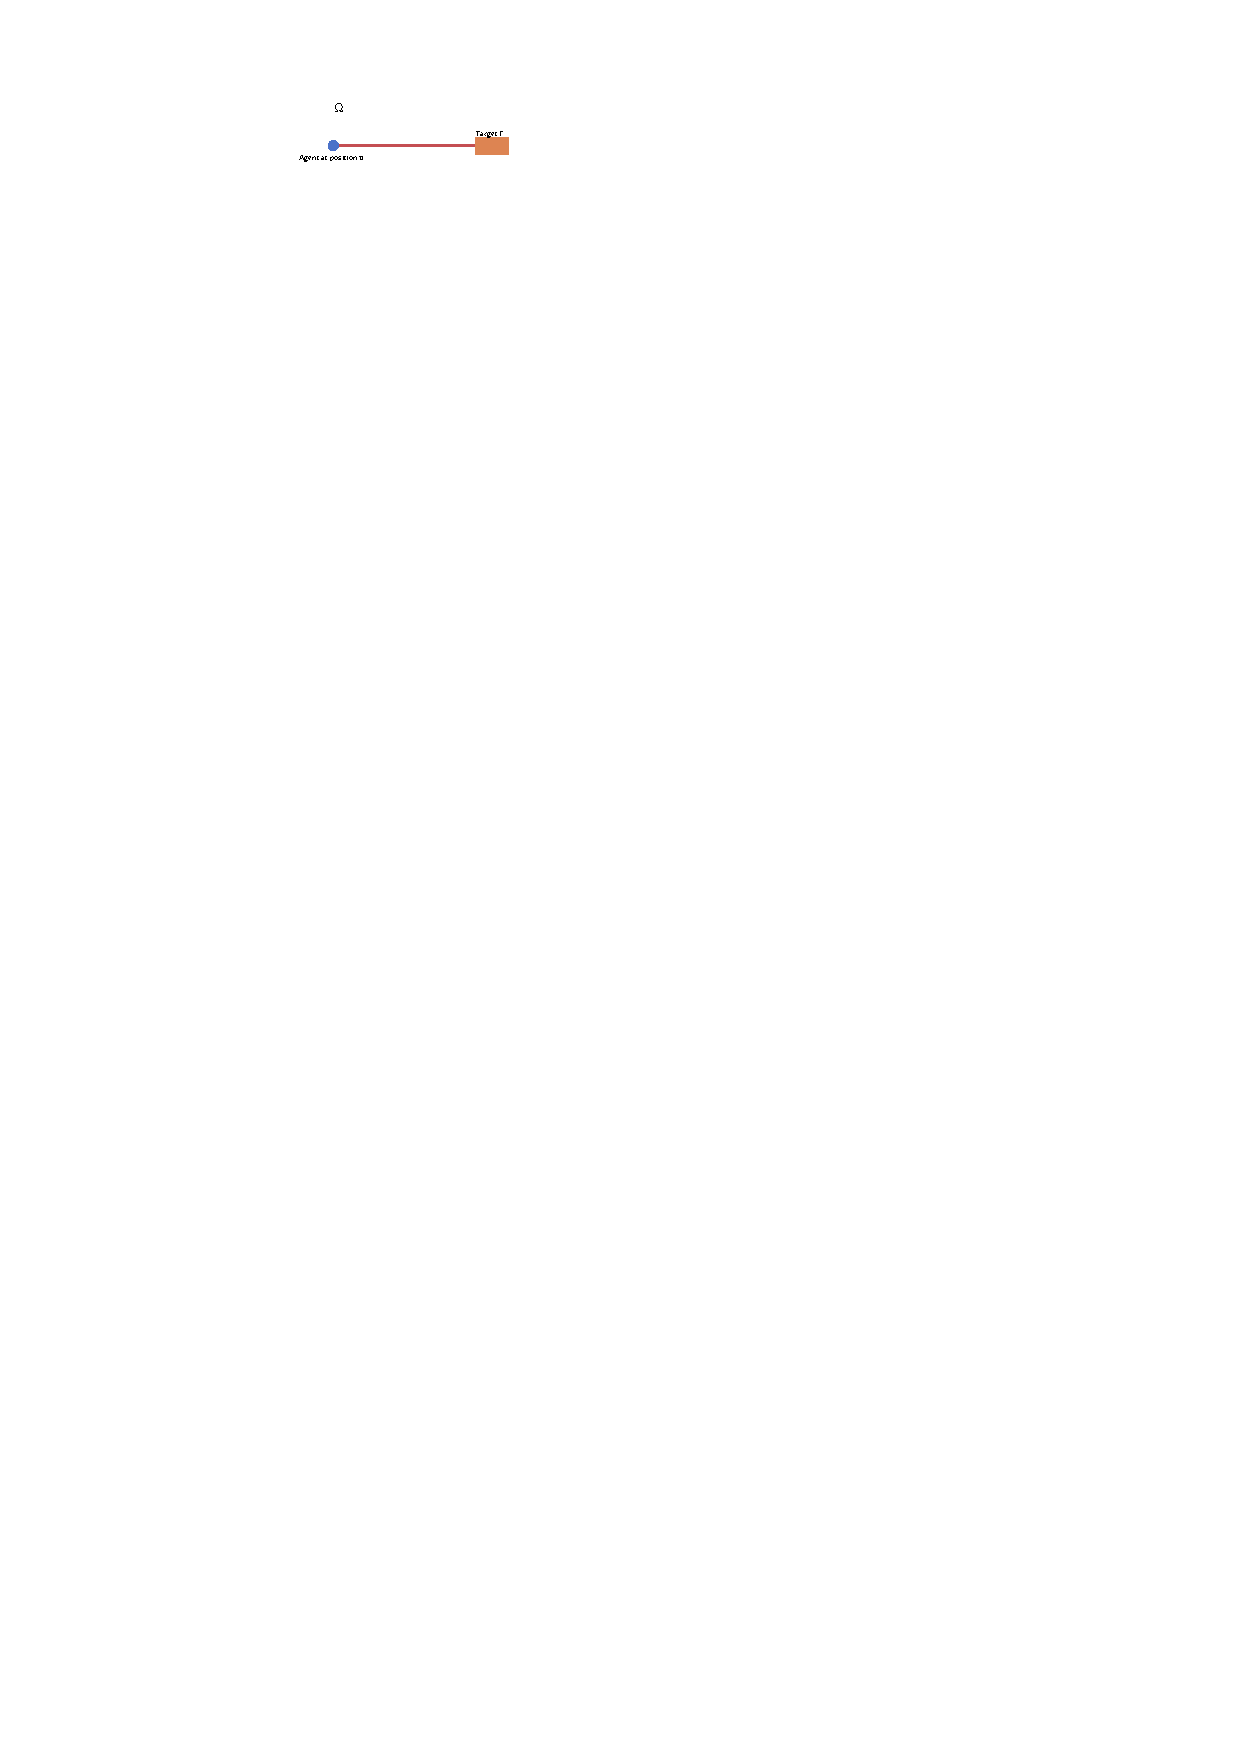
\includegraphics[width=0.45\textwidth]{./figs/euclid_en.pdf}}
		\hfill
		\subfigure[Follow {\color{red}?}]{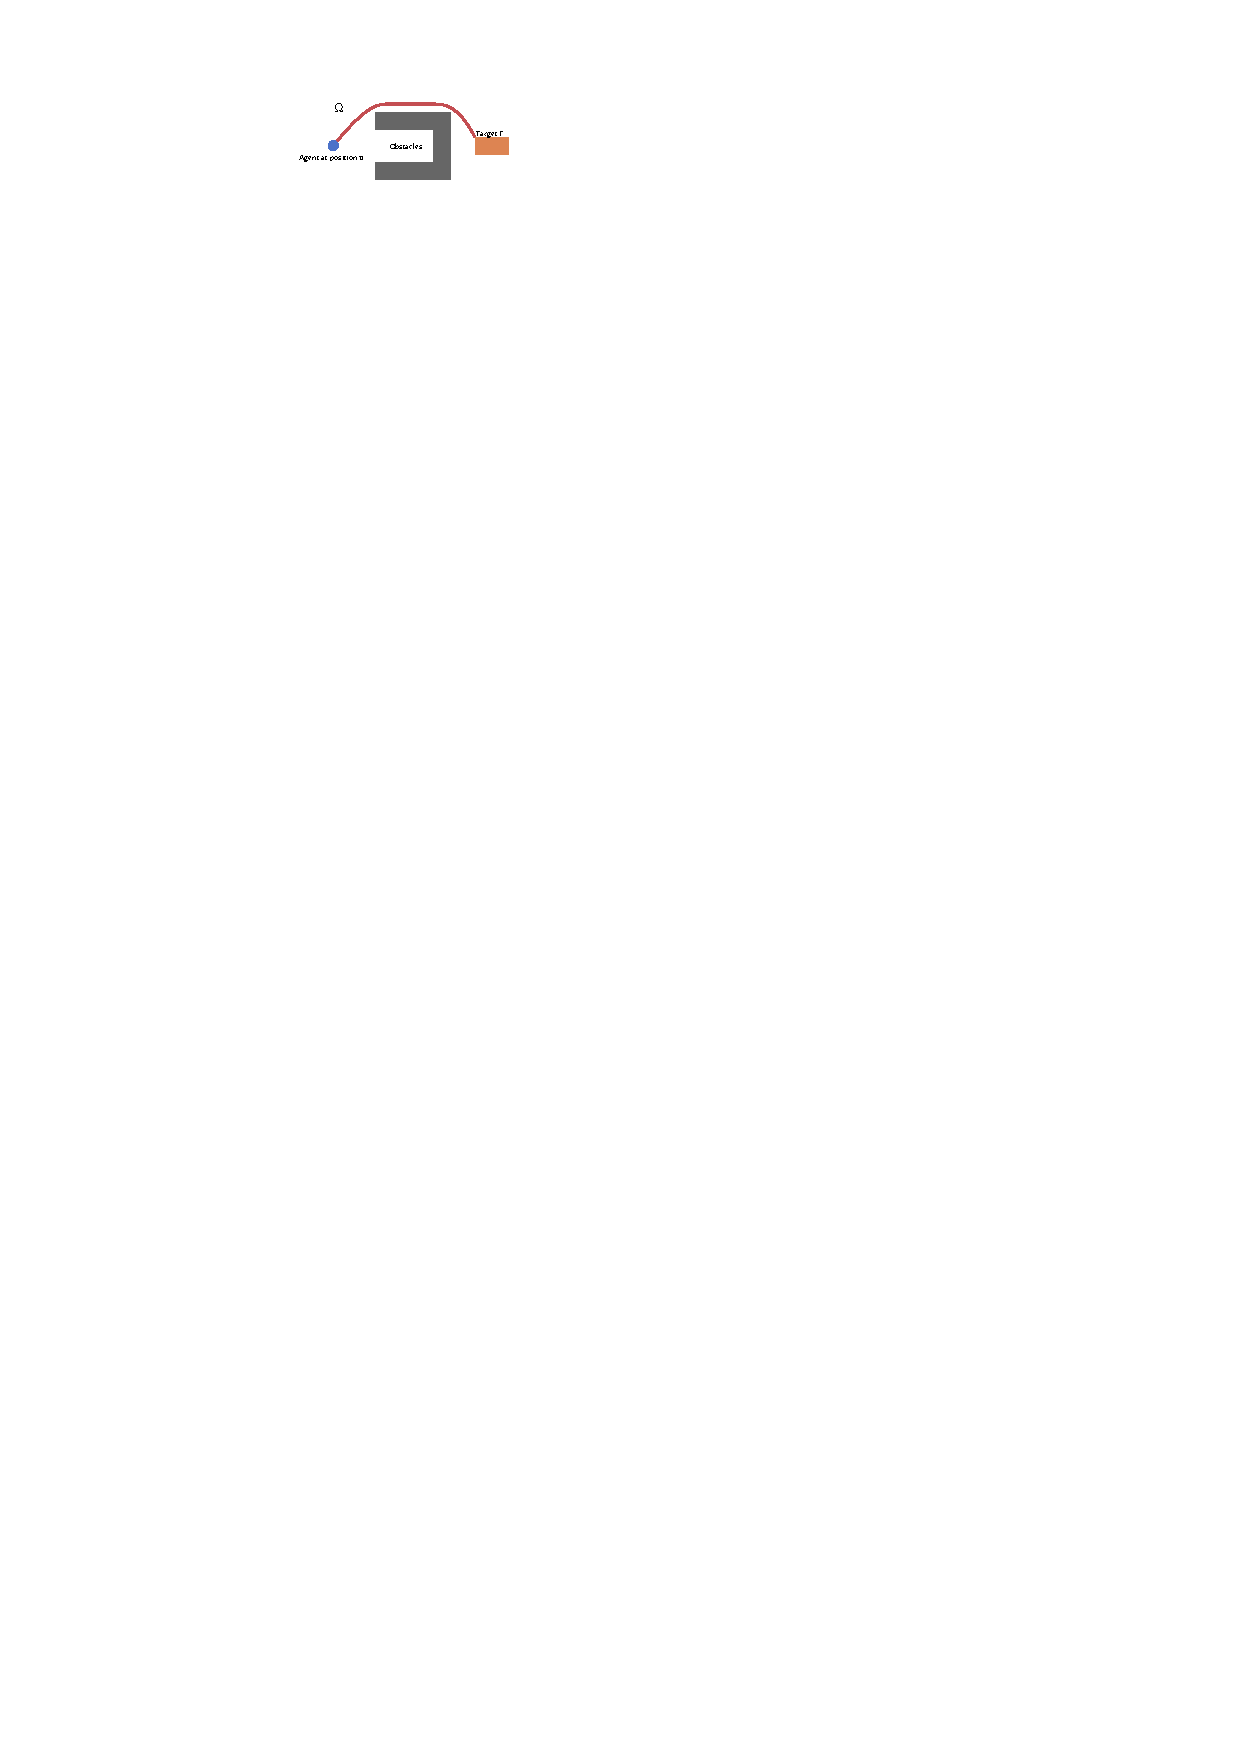
\includegraphics[width=0.45\textwidth]{./figs/chicken_en.pdf}}
	\end{figure}
\end{frame}

\section{Navigation on a Ragular Graph}
\begin{frame}[plain]
	\begin{center}
		{\color{myblue} \huge Navigating through a (Ragular) Graph}
	\end{center}
\end{frame}

\begin{frame}
	\frametitle{Discretization}
	Let us first assume we discretize our domain into a regular grid
	\begin{equation*}
		\domain_{h} \subset \left\{ (i \cdot h, j \cdot h) \ | \ i, j \in \mathbb{N} \right\}
	\end{equation*}
	and let us assume we have one of the following neighborhood relations
		\begin{figure}
		\subfigure[Von Neumann]{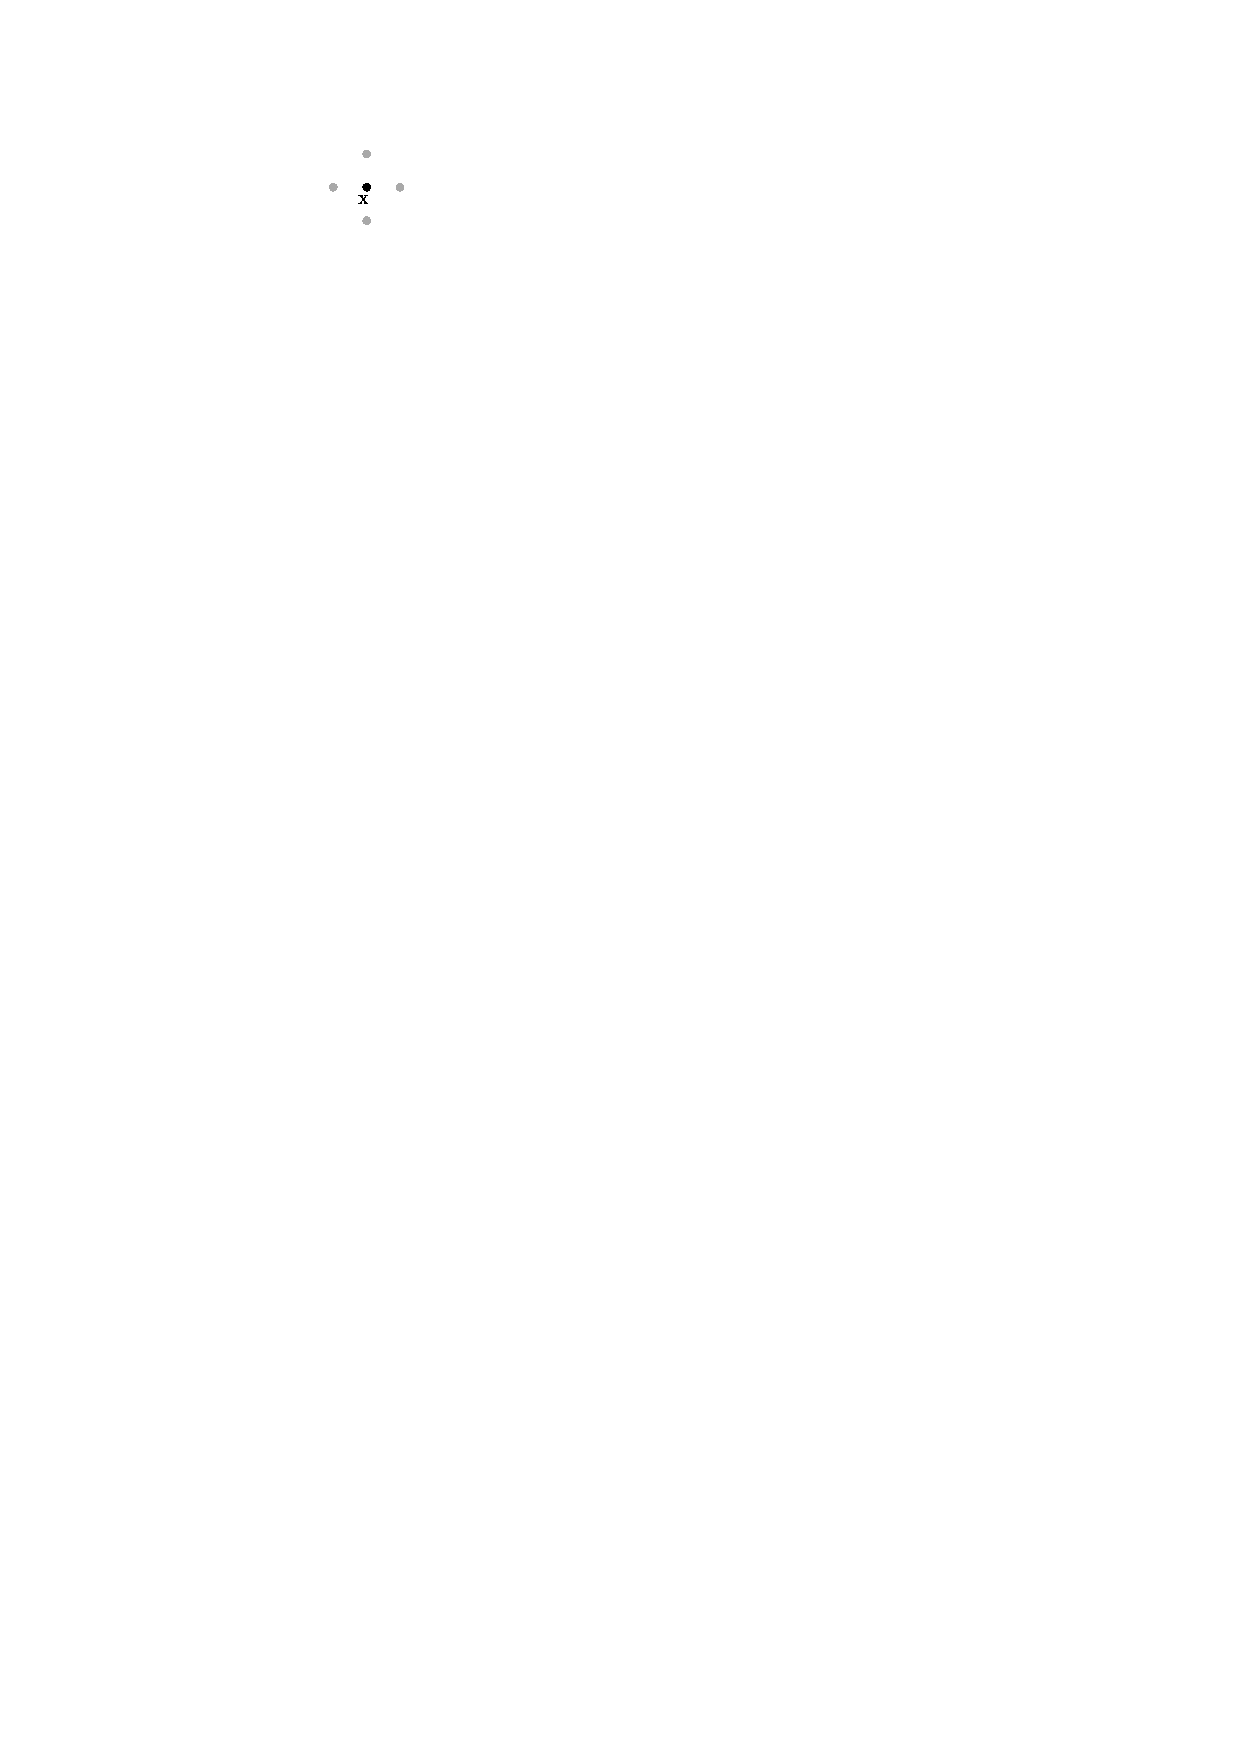
\includegraphics[width=0.150\textwidth]{./figs/neumann-nh.pdf}}
		\hspace{3cm}
		\subfigure[Moore]{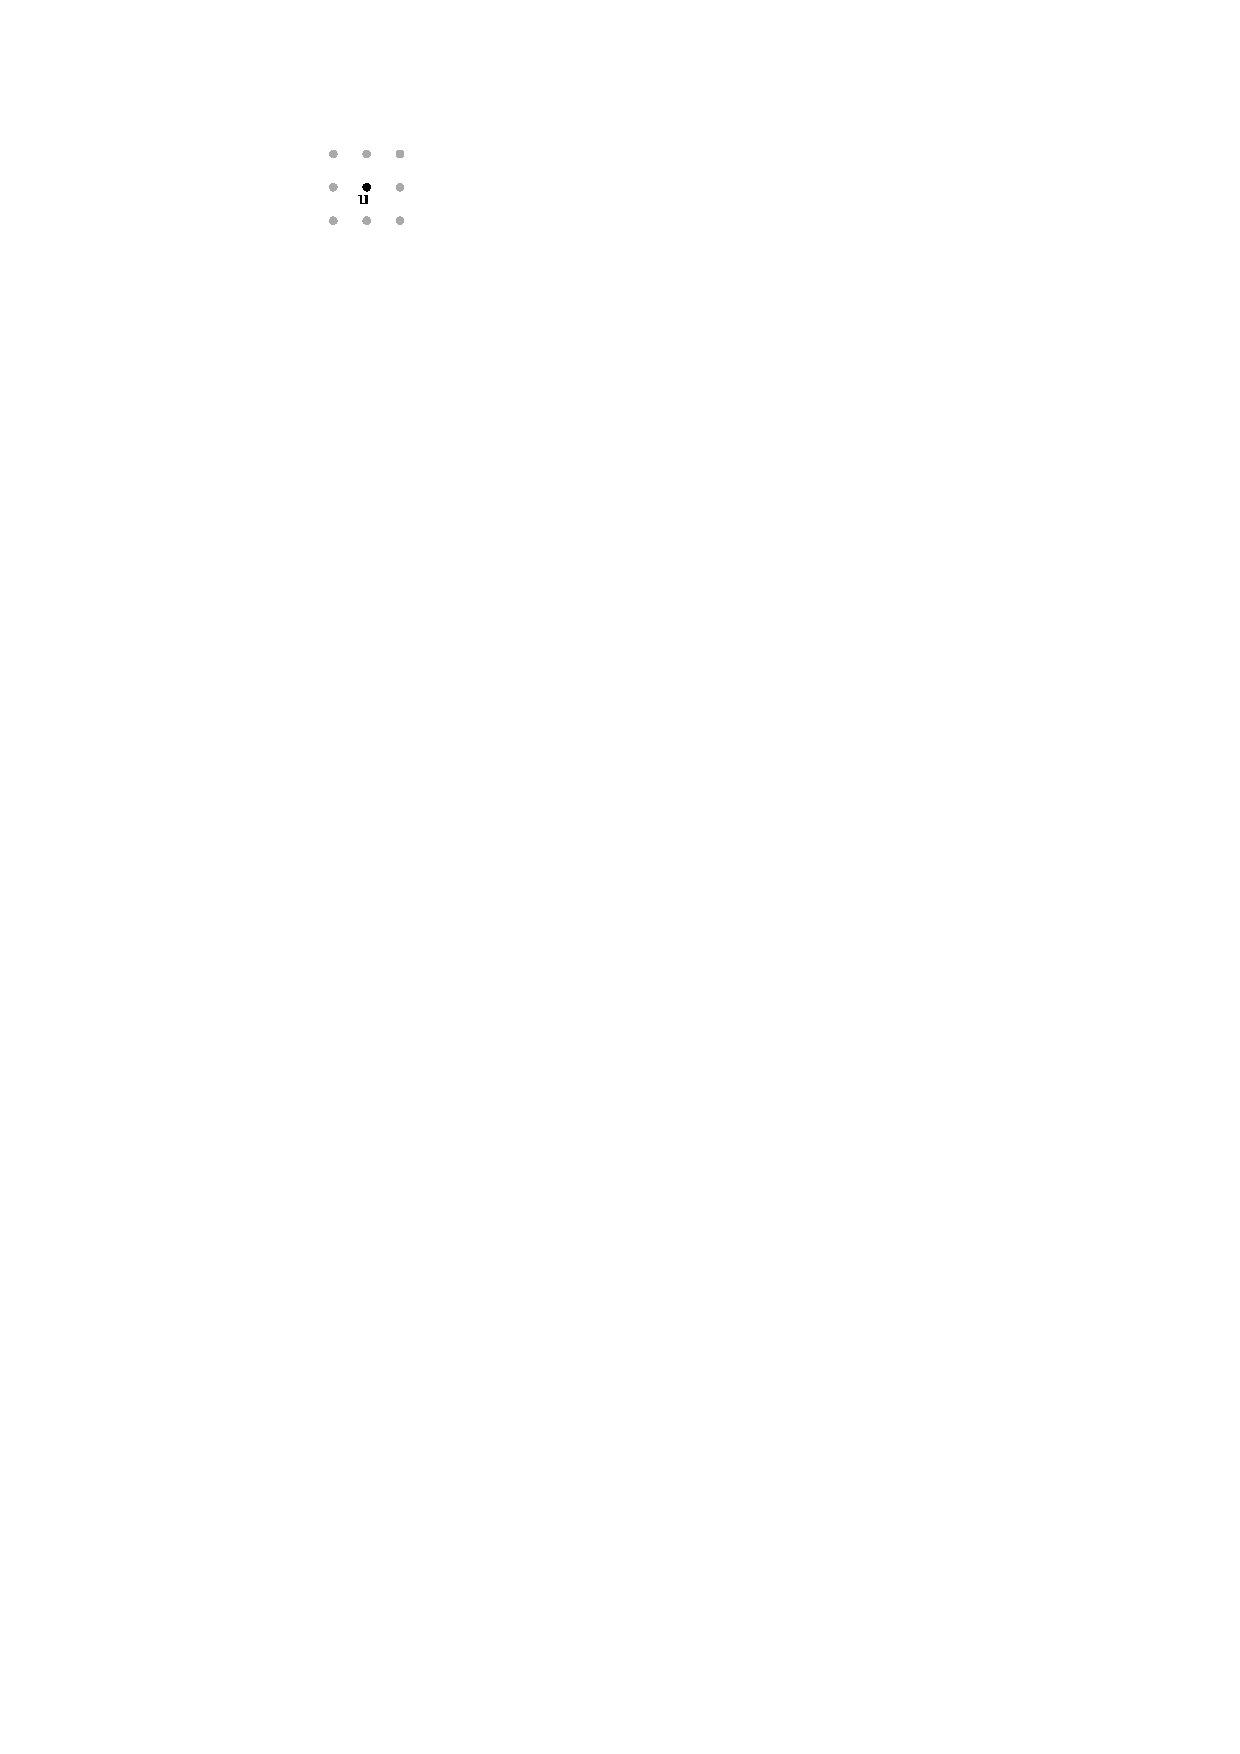
\includegraphics[width=0.150\textwidth]{./figs/moore-nh.pdf}}
	\end{figure}
	such that we can only walk on the edges of the graph.
\end{frame}

\begin{frame}
	\frametitle{Discretization}
	In this case, the problems is equivalent to the problem of finding the shortest path from $\uu$ to $\osmDestination_h$ on a graph!
	\begin{figure}
		\centering
		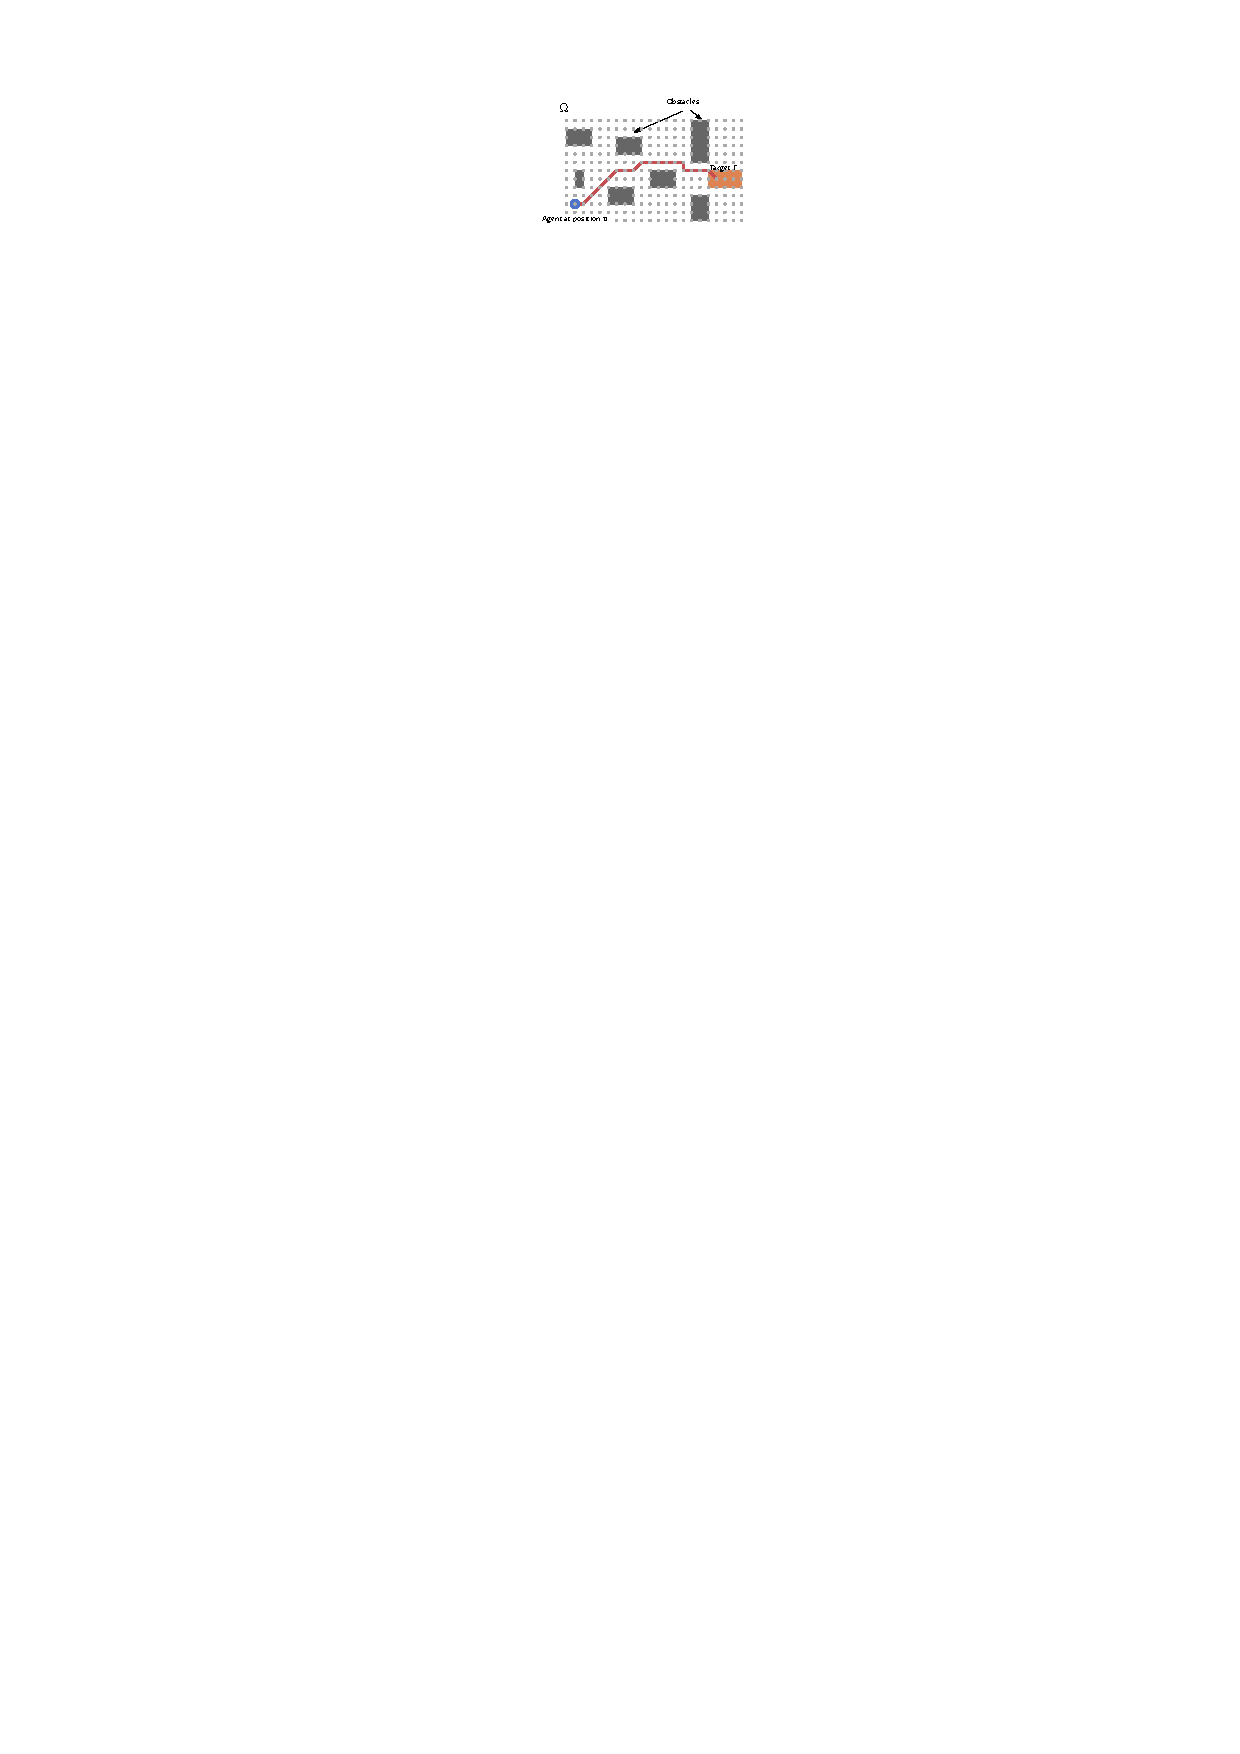
\includegraphics[width=0.6\textwidth]{./figs/wayfinding-in-Z_en.pdf}
	\end{figure}
	$\Rightarrow$ Dijkstra's \cite{dijkstra-1959} algorithm provides a solution.
\end{frame}

\subsection{Dijkstra's Algorithm}
\begin{frame}[plain]
	\begin{center}
		{\color{myblue} \huge Dijkstra's Algorithm}
	\end{center}
\end{frame}

\begin{frame}
	\frametitle{Dijkstra's Algorithm}
	\textbf{Strategy}: Compute the shortest path for all grid points $\uu \in \domain$ starting at $\osmDestination_h$ using \textsc{Dijkstra} \cite{dijkstra-1959}.\\
	\vspace{1cm}
	
	\uncover<2>{\textbf{Observation}: If $\uu_0, \ldots, \uu_k$ is the shortest path from $\uu_0$ to $\uu_k$ and $,\uu_k, \ldots, ,\uu_m$ is the shortest path from $,\uu_k$ to $,\uu_m$, then
		\begin{equation*}
			\uu_0, \ldots, \uu_m
		\end{equation*}
		is the shortest path from $\uu_0$ to $\uu_m$.}
\end{frame}

\begin{frame}
	\frametitle{Dijkstra's Algorithm}
	\textbf{Definitions}: 
	\begin{enumerate}[label=(\roman*)]
		\item $\uu, \vvv$: Nodes of the grid
		\item $d_{\osmDestination_h}(\uu)$: Distance between $\uu$ and $\osmDestination_h$ along the shortest path
		\item $d(\uu, \vvv)$: Distance between $\uu$ and $\vvv$ / weight of the edge $(\uu, \vvv)$
		\item $d_{\uu}$: Distance between $\uu$ and $\osmDestination_h$ computed by the algorithm
		\item $\mathcal{Q}$: A \textsc{PriorityQueue} (e.\,g. \textsc{FibonacciHeap})
	\end{enumerate}
\end{frame}

%\begin{frame}
%	\frametitle{Dijkstra's Algorithm}
%	
%\end{frame}

\begin{frame}[fragile]
	\frametitle{Dijkstra's Algorithm}
		\begin{columns}
		\begin{column}{0.4\textwidth}
			{ \scriptsize
			\begin{algorithm}[H]
			\KwIn{$\domain_h, \osmDestination_h, d$}
			\KwOut{$d_{\osmDestination_h}$}
			$d_{\uu} \leftarrow \infty$ for all $\uu \in \domain_h$\;
			$d_{\uu} \leftarrow 0$ for all $\uu \in \osmDestination_h$\;
			$\mathcal{Q} \leftarrow \left\{ (\uu, d_{\uu}) \in \osmDestination_h \right\}$\;
			\While{$\mathcal{Q} \neq \emptyset$}{
				$(\uu, d_{\uu}) \leftarrow \mathcal{Q}.\textsc{pop()}$\;
				\ForEach{\text{neighbour} $\vvv$ \text{of} $\uu$}{
					$uv \leftarrow d_\uu + d(\uu, \vvv)$\;
					\If{$uv < d_{\vvv}$}{
						$d_{\vvv} \leftarrow uv$\;
						\eIf{$(\vvv, d_\vvv) \in \mathcal{Q}$}{
							$\mathcal{Q}.\textsc{decrease}(\vvv, d_\vvv)$\;
						}
						{
							$\mathcal{Q}.\textsc{push}(\vvv, d_\vvv)$\;
						}
					}
				}
			}
			$d_{\osmDestination_h} \leftarrow \left\{ (\uu, d_{\uu} \ | \ \uu \in \domain_h) \right\}$\;
			\textbf{return} $d_{\osmDestination_h}$\;
		\end{algorithm}
		}
		\end{column}
		\begin{column}{0.6\textwidth}
			\uncover<1->{$\mathcal{Q}$ is sorted according to the current distance values {\color{myblue}$d_\vvv$}:  
			\begin{enumerate}[label=$\bullet$]
				\item $\mathcal{Q}.\textsc{pop}()$, gives us the the smalles element,
				\item $\mathcal{Q}.\textsc{decrease}(\vvv, d_\vvv)$ changes the element,
				\item and $\mathcal{Q}.\textsc{push}(\vvv, d_\vvv)$ adds a new element
			\end{enumerate}}
			\vspace{1cm}
			\uncover<2->{\textbf{Complexity:}%(for a simple graph with positive weights and $n$ nodes)
			\begin{enumerate}[label=$\bullet$]
				\item Time: $\mathcal{O}(n\log(n))$
				\item Memory: $\mathcal{O}(n)$
			\end{enumerate}}
			%\textbf{Invarianz}: Für alle $\xx \in \domain$, die nicht in $\mathcal{Q}$ enthalten sind, ist $d_{\osmDestination}(\xx)$ ist der kürzeste Pfad von $\xx$ nach $\osmDestination$. 
		\end{column}
	\end{columns}
\end{frame}


\begin{frame}
	\frametitle{Dijkstra's Algorithm}
	\textbf{Strategy}: Compute the shortest path for all grid points $\uu \in \domain$ to starting at $\osmDestination_h$ using \textsc{Dijkstra} \cite{dijkstra-1959}.\\
	\vspace{1cm}
	
	\textbf{Observation}: If $\uu_0, \ldots, \uu_k, \ldots,\uu_m$ is the shortest path from $\uu_0$ to $\uu_m$, then
		\begin{equation*}
			\uu_0, \ldots, \uu_k
		\end{equation*}
		is the shortest path from $\uu_0$ to $\uu_k$.\\
	\vspace{1cm}
	
	\uncover<2->{\textbf{Invariance}: 
	Whenever $d_\uu$ gets removed from $\mathcal{Q}$ in line 5, it is the distance of the shortest path for all $\uu$ to $\domain_h$ (proof by induction).}
\end{frame}

\subsection{A$^*$ Algorithm}
\begin{frame}[plain]
	\begin{center}
		{\color{myblue} \huge A$^*$ Algorithm}
	\end{center}
\end{frame}

\begin{frame}
	\frametitle{A$^*$ Algorithm}
	What if we only want to compute the shortest path from $\uu^*$ to $\osmDestination_h$.\\
	\vspace{1cm}
	How can we avoid computing distances for points that are located in the opposite direction?
\end{frame}

%\begin{frame}
%	\frametitle{A$^*$ Algorithm}
%	
%\end{frame}

%\begin{frame}
%	\frametitle{A$^*$ Algorithm}
%	A$^*$ uses a heuristic $h$ to estimate the cost / distance to the target. This heuristic has to have two properties:
%	\begin{enumerate}[label=(\arabic*)]
%		\item It never overestimates the actual cost / distance (adnssible), that is,
%		$$h(\uu) \leq d_{\osmDestination_h}(\uu).$$
%		\item It is monotone, or consistent, that is
%		$$h(\uu) \leq d(\uu, \vvv) + h(\vvv)$$
%		for every edge $(\uu, \vvv)$.
%	\end{enumerate}
%	If we want to compute the distance to $\uu$, we can use $h_\uu(\vvv) = \Vert \vvv - \uu \Vert$ as our heursitic.
%\end{frame}

\begin{frame}
	\frametitle{A$^*$ Algorithm}
	\textbf{Strategy}: 
	Compute ``towards'' $\uu^* \in \domain_h$ first \cite{hart-1968}.\\
	\vspace{0.5cm}
	
	\uncover<2->{\textbf{Observation (1)}: The Euclidean distance $\Vert \uu_0 - \uu_m \Vert$ is a lower bound of the distance between $\uu_0$ and $\uu_m$, that is,
	\begin{equation*}
			\Vert \uu_0 - \uu_m \Vert \leq \sum_{i=0}^{m-1} d(\uu_i, \uu_{i+1}) =  \sum_{i=0}^{m-1}  \Vert \uu_i -  \uu_{i+1} \Vert,
	\end{equation*}}
	\uncover<3->{\textbf{Observation (2)}: If 
	\begin{equation*}
			d_{\osmDestination_h}(\vvv) + \Vert \uu^* - \vvv  \Vert > d_{\osmDestination_h}(\uu^*)
	\end{equation*}
	holds, then the shortest path from $\osmDestination_h$ to $\uu^*$ does not consists of $\vvv$.}\\
	\vspace{0.5cm}
	\uncover<3->{$\Rightarrow$ Sort the heap by $d_{\osmDestination_h}(\vvv) + \Vert \uu^* - \vvv  \Vert$ instead of $d_{\osmDestination_h}(\vvv)$.}
\end{frame}

%\begin{frame}
%	\frametitle{A$^*$ Algorithm}
%	
%\end{frame}

%\begin{frame}
%	\frametitle{A$^*$ Algorithm}
%	Let $\uu, \uu_1, \uu_2 \in \domain_{h}$ then
%	\begin{equation*}
%		d_{\osmDestination_h}(\uu_1) + \Vert \uu - \uu_1 \Vert \leq d_{\osmDestination_h}(\uu_2) + \Vert \uu - \uu_2 \Vert \iff d_{\osmDestination_h}(\uu_1) \leq d_{\osmDestination_h}(\uu_2)
%	\end{equation*}
%	holds.
%\end{frame}


%\begin{frame}
%	\frametitle{A$^*$ Algorithm}	
%		\vspace{-0.5cm}
%		\begin{columns}
%		\begin{column}{0.4\textwidth}
%			\begin{figure}
%			\centering
%			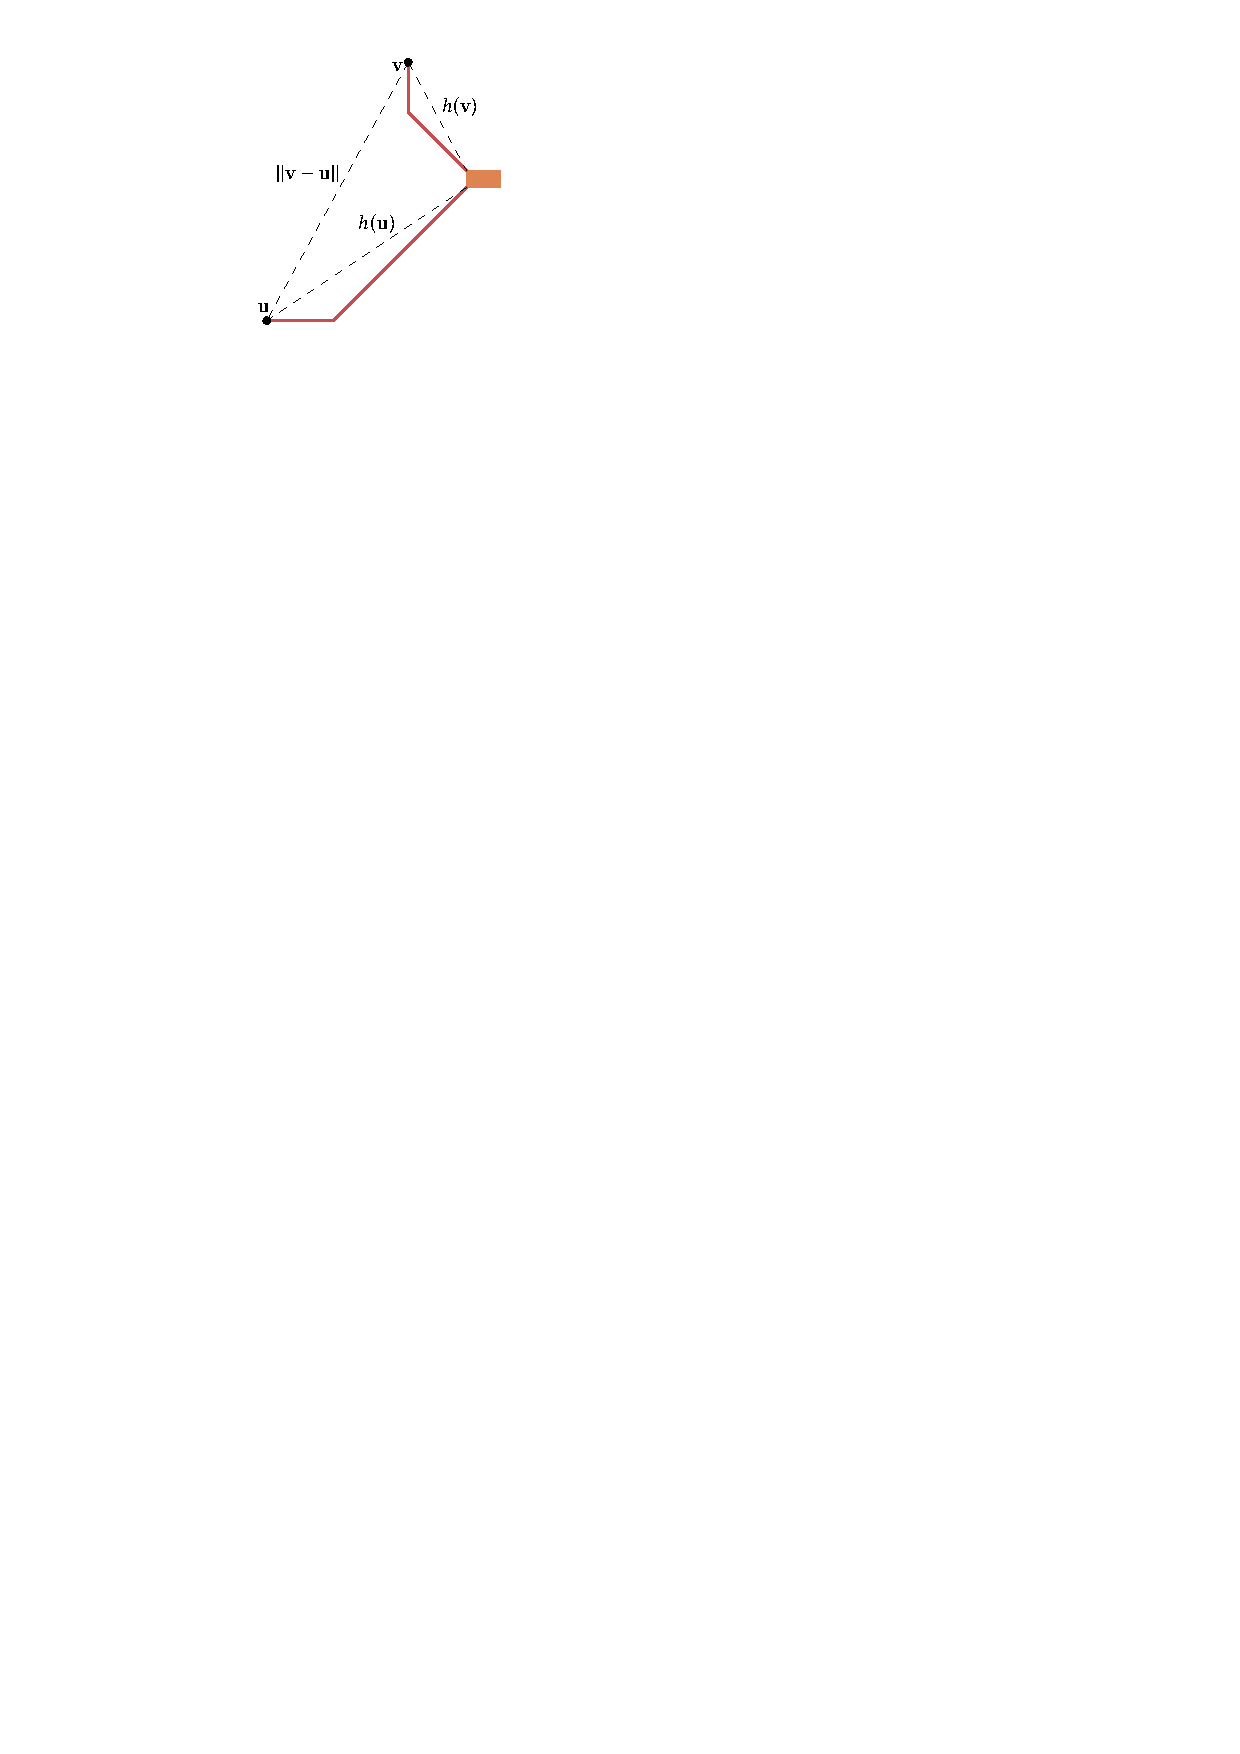
\includegraphics[width=0.8\textwidth]{./figs/a-star-obs.pdf}
%		\end{figure}
%		\end{column}
%		\hfill
%		\begin{column}{0.4\textwidth}
%			\uncover<1->{Let us define 
%			\begin{equation*}
%				h(\uu) := \_{\vvv \in \osmDestination} \Vert \uu - \vvv \Vert,
%			\end{equation*}
%			then 
%			\begin{equation*}
%				h(\uu) - h(\vvv) \leq \Vert \vvv - \uu \Vert.
%			\end{equation*}
%			holds.}
%		\end{column}
%	\end{columns}
%	\vspace{0.5cm}
%	
%	\uncover<1->{\textbf{Observation (2*)}: If  
%	\begin{equation*}
%		d_{\osmDestination_h}(\vvv) + h(\uu) - h(\vvv) > d_{\osmDestination_h}(\uu) \iff d_{\osmDestination_h}(\vvv) + h(\uu) > d_{\osmDestination_h}(\uu) +  h(\vvv) 
%	\end{equation*}
%	holds, then the shortest path from $\osmDestination_h$ to $\uu$ does not consist of $\vvv$.}
%\end{frame}

\begin{frame}[fragile]
	\frametitle{A$^*$ Algorithm}
	\begin{columns}
		\begin{column}{0.4\textwidth}
			{\scriptsize
			\begin{algorithm}[H]
				\KwIn{$\domain_h, \osmDestination_h, d, \uu^*$}
				\KwOut{$d_{\osmDestination_h}(\uu^*)$}
				$d_{\uu} \leftarrow \infty$ for all $\uu \in \domain_h$\;
				$d_{\uu} \leftarrow 0$ for all $\uu \in \osmDestination_h$\;
				\tcc{\color{myblue}sort by $d_{\uu} + \Vert \uu - \uu^* \Vert$}
				$\mathcal{Q} \leftarrow \left\{ (\uu, d_{\uu} \right\}$\;
				\While{$\mathcal{Q} \neq \emptyset$}{
					$(\uu, d_{\uu}) \leftarrow \mathcal{Q}.\textsc{pop()}$\;
					{\color{myblue}\If{$\uu = \uu^*$}{
						\textbf{return} $d_{\uu}$\;
					}}
					\ForEach{neighbour $\vvv$ of $\uu$}{
						$uv \leftarrow d_{\uu} + d(\uu, \vvv)$\;
						\If{$uv < d_\vvv$}{
							$ d_\vvv \leftarrow uv$\;
							\eIf{$(\vvv,  d_\vvv) \in \mathcal{Q}$}{
								$\mathcal{Q}.\textsc{decrease}(\vvv,  d_\vvv)$\;
							}
							{
								$\mathcal{Q}.\textsc{push}(\vvv,  d_\vvv)$\;
							}
						}
					}
				}
			\end{algorithm}
		
		}
		\end{column}
		\begin{column}{0.6\textwidth}
			\uncover<1->{$\mathcal{Q}$ sorted according to the current distance values {\color{myblue}  $d_\vvv + \Vert \vvv - \uu^* \Vert$}:
		\begin{enumerate}[label=$\bullet$]
			\item $\mathcal{Q}.\textsc{pop}()$, gives us the the smalles element
			\item $\mathcal{Q}.\textsc{decrease}(\vvv, d_\vvv)$ changes the element
			\item und $\mathcal{Q}.\textsc{push}(\vvv, d_\vvv)$ adds a new element
		\end{enumerate}}
		\vspace{1cm}
		\uncover<2->{\textbf{Complexity:}%(for a simple graph with positive weights and $n$ nodes)
		\begin{enumerate}[label=$\bullet$]
			\item Time: $\mathcal{O}(n\log(n))$
			\item Memory: $\mathcal{O}(n)$
		\end{enumerate}}
			%\textbf{Invarianz}: Für alle $\xx \in \domain$, die nicht in $\mathcal{Q}$ enthalten sind, ist $d_{\osmDestination}(\xx)$ ist der kürzeste Pfad von $\xx$ nach $\osmDestination$. 
		\end{column}
	\end{columns}
\end{frame}

\begin{frame}
	\frametitle{A$^*$ Algorithms}	
	\textbf{Choice of a heuristic}: The Euclidean distance $h(\vvv) := \Vert \vvv - \uu^*\Vert$ works in our case but other heuristics might be possible.
	 If 
	\begin{equation*}
		\begin{split}
			\uncover<2->{h(\vvv) & \leq d_{\osmDestination}(\vvv) \quad \quad \quad \ \  \text{ (admissible)}}\\
			\uncover<3->{h(\vvv) & \leq d(\vvv, \uu) + h(\uu) \text{ (monoton)}}
		\end{split}
	\end{equation*}
	\uncover<3->{holds for each node $\uu$ and edge $(\uu, \vvv)$, then $h$ is \textbf{consistent} and A$^*$ finds the shortest path without visiting nodes multipe times.}\\
	\vspace{1cm}
	\uncover<4->{\textbf{Lost advantage}: If you have to compute the distance for all nodes, A$^*$ has no advantage over \textsc{Dijkstra}.}
\end{frame}

\section{Navigating through the Continuous Space}
\begin{frame}[plain]
	\begin{center}
		{\color{myblue} \huge Navigating through the Continuous Space}
	\end{center}
\end{frame}

%\subsection{Defining the Problem}
\begin{frame}
	\frametitle{Defining the Problem}
	What we are looking for a \textbf{distance function} 
	
	$$d_{\osmDestination}: \mathbb{R}^2 \rightarrow \mathbb{R}$$
	
	that gives us the distance to our target region $\osmDestination$ for any position $\uu$  in our spatial domain $\domain$.
	\begin{figure}
		\centering
		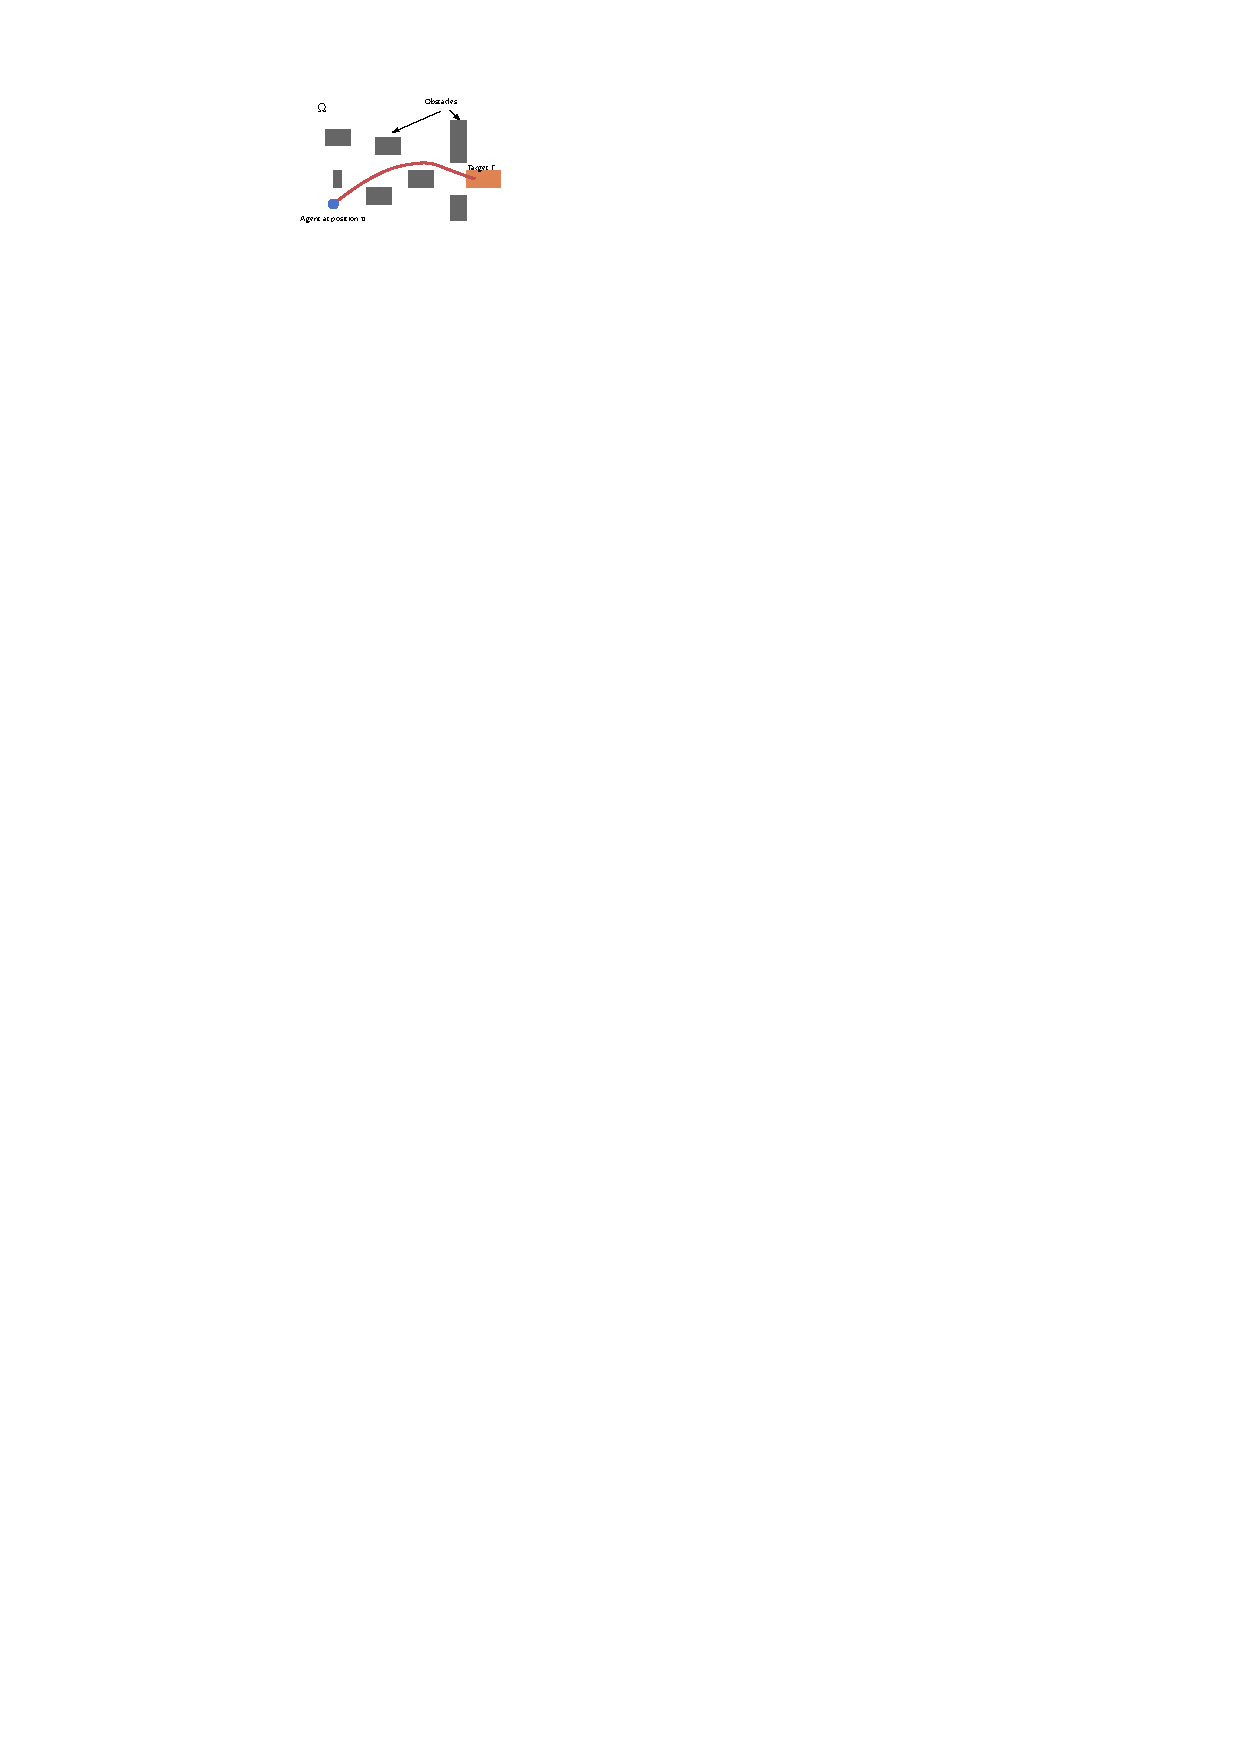
\includegraphics[width=0.4\textwidth]{./figs/wayfinding_en.pdf}
	\end{figure}
	The gradient of this distance functions $-\nabla d_{\osmDestination}$ gives us the direction in which we or the agent should move.
\end{frame}

\begin{frame}
	\frametitle{Defining the Problem}
	If there is no obstacle ``in the way'', then an appropriate distance function is the Euclidean distance
	
	$$d_{\osmDestination}(\uu) = \min_{\vvv \in \osmDestination} \Vert \uu - \vvv\Vert$$
	
	and the \textbf{shortest path} from $\osmDestination$ to $\uu$ follows the gradient $-\nabla d_{\osmDestination}$:
	\begin{figure}
		\subfigure[Follow $-\nabla d_{\osmDestination}$]{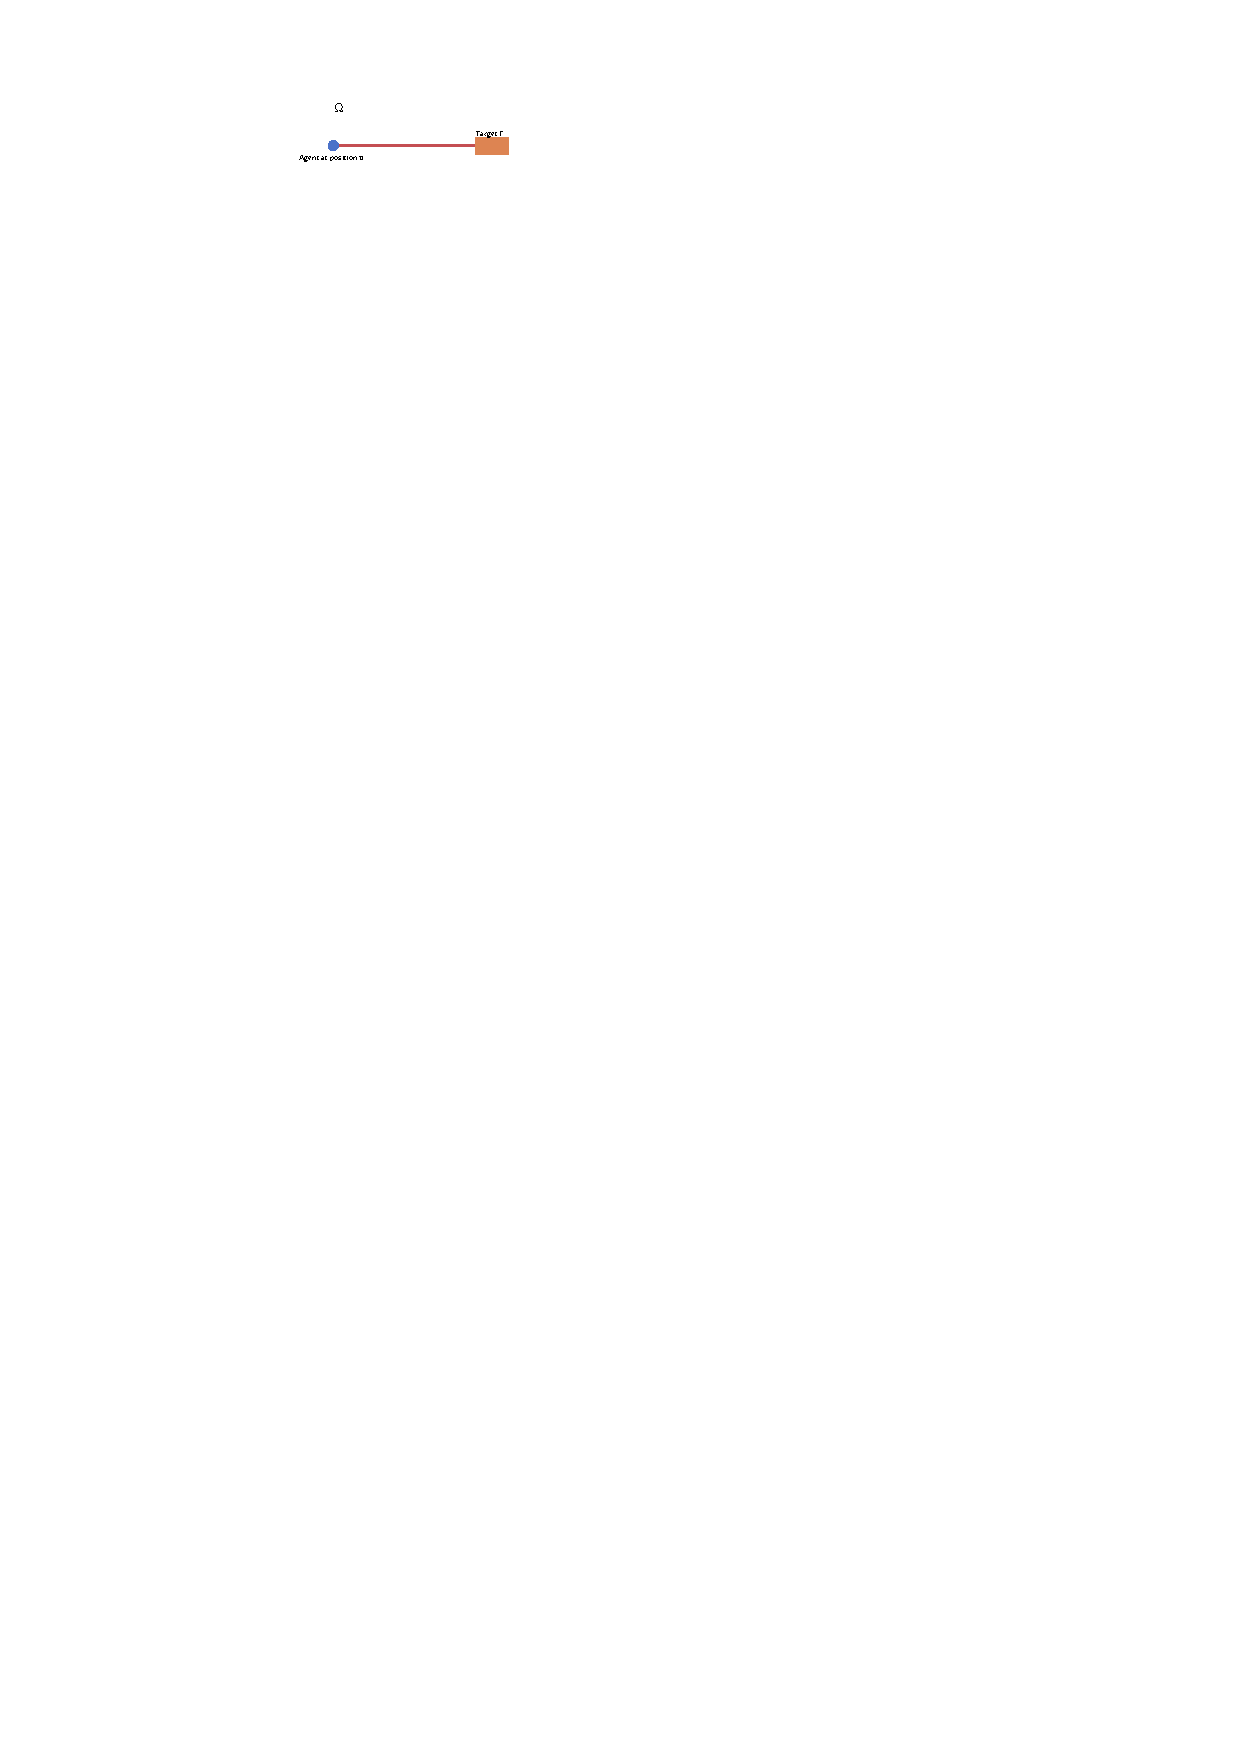
\includegraphics[width=0.45\textwidth]{./figs/euclid_en.pdf}}
		\hfill
		\subfigure[Follow {\color{red}?}]{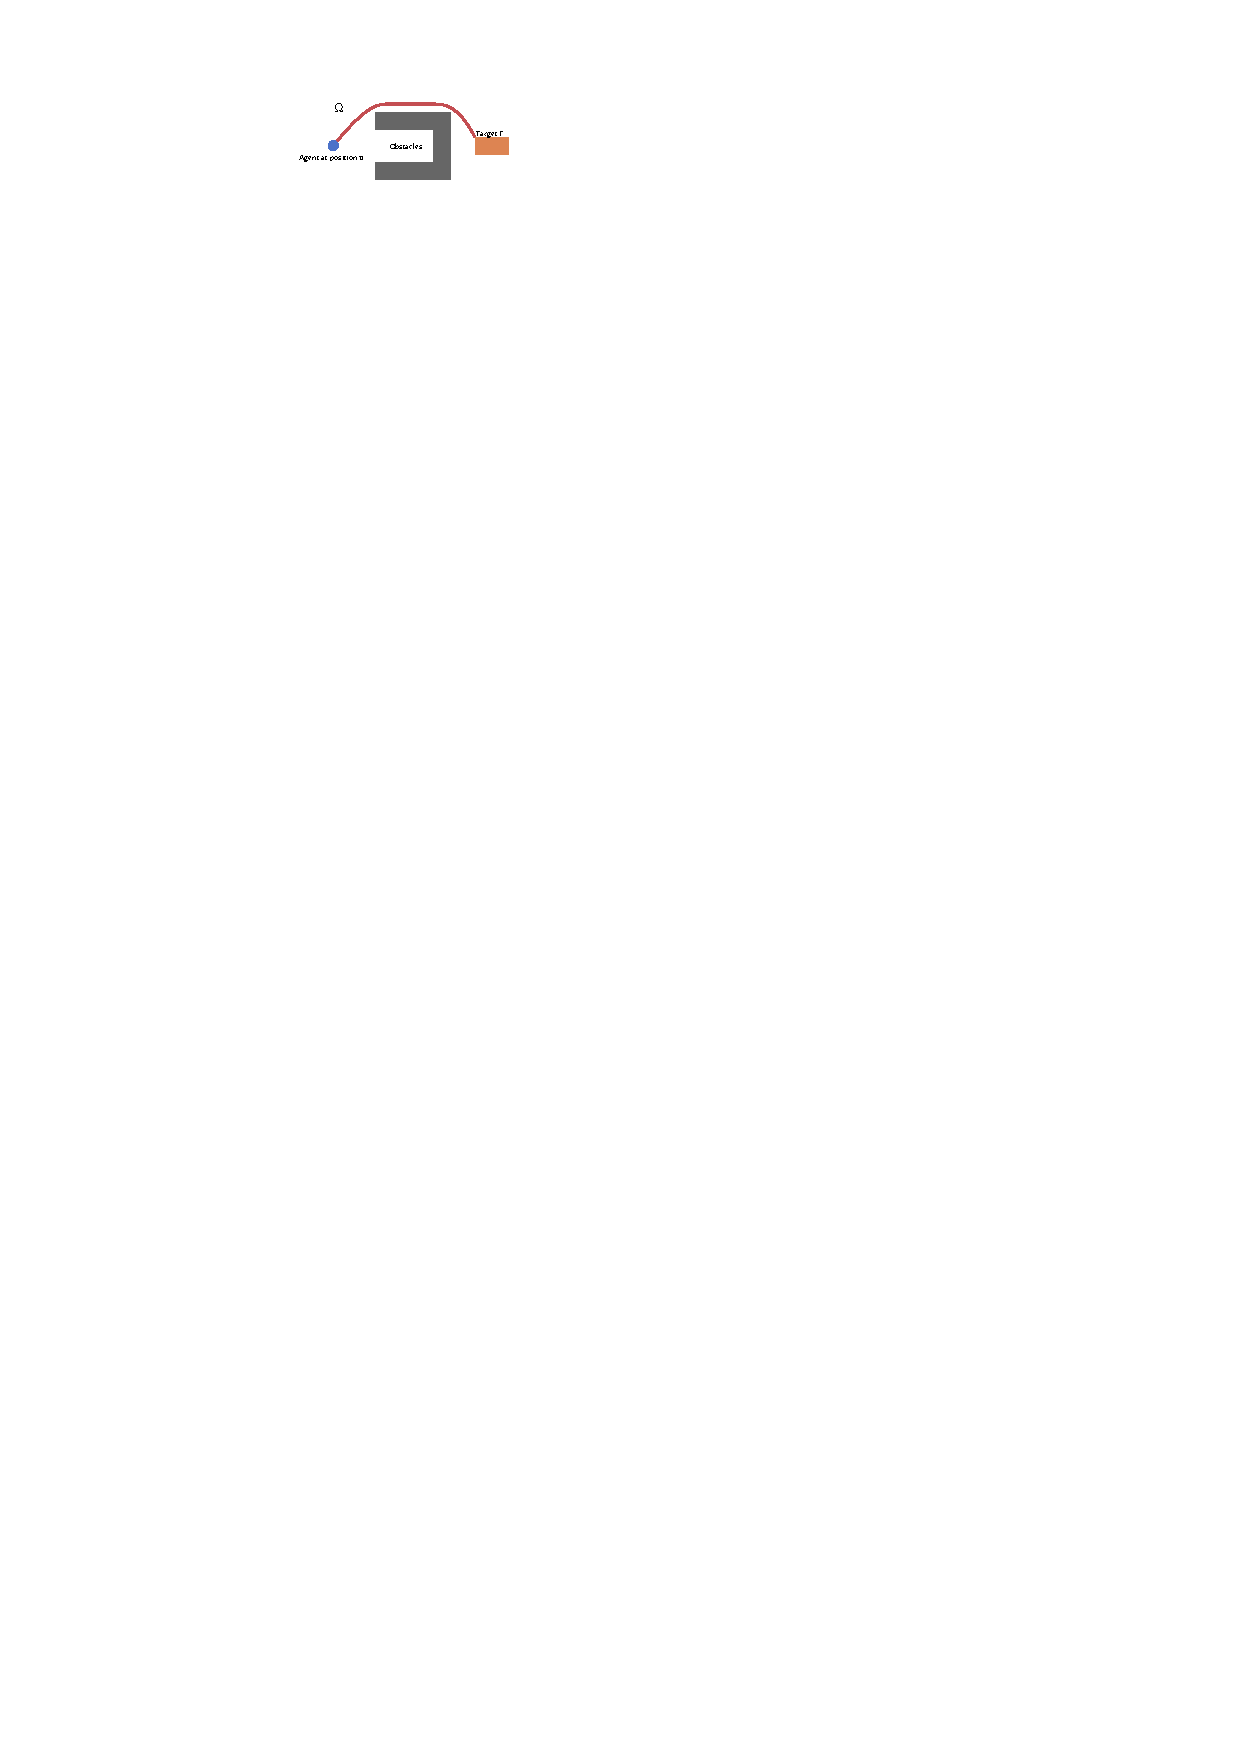
\includegraphics[width=0.45\textwidth]{./figs/chicken_en.pdf}}
	\end{figure}
\end{frame}

\subsection{The Eikonal Equation}
\begin{frame}[plain]
	\begin{center}
		{\color{myblue} \huge The Eikonal Equation}
	\end{center}
\end{frame}

\begin{frame}
	\frametitle{The Eikonal Equation}
	We imagine a \textbf{wavefront} propagating with a \textbf{travel speed} $f(\uu) = 1$.
	It starts at the target $\osmDestination$ and propagates through the region $\domain$.\\
	\vspace{0.25cm}
	
	\uncover<2->{$T(\uu)$ is the \textbf{travel time} or arrival time of the \textbf{wavefront} at the location $\uu$.}
	
	\begin{figure}
		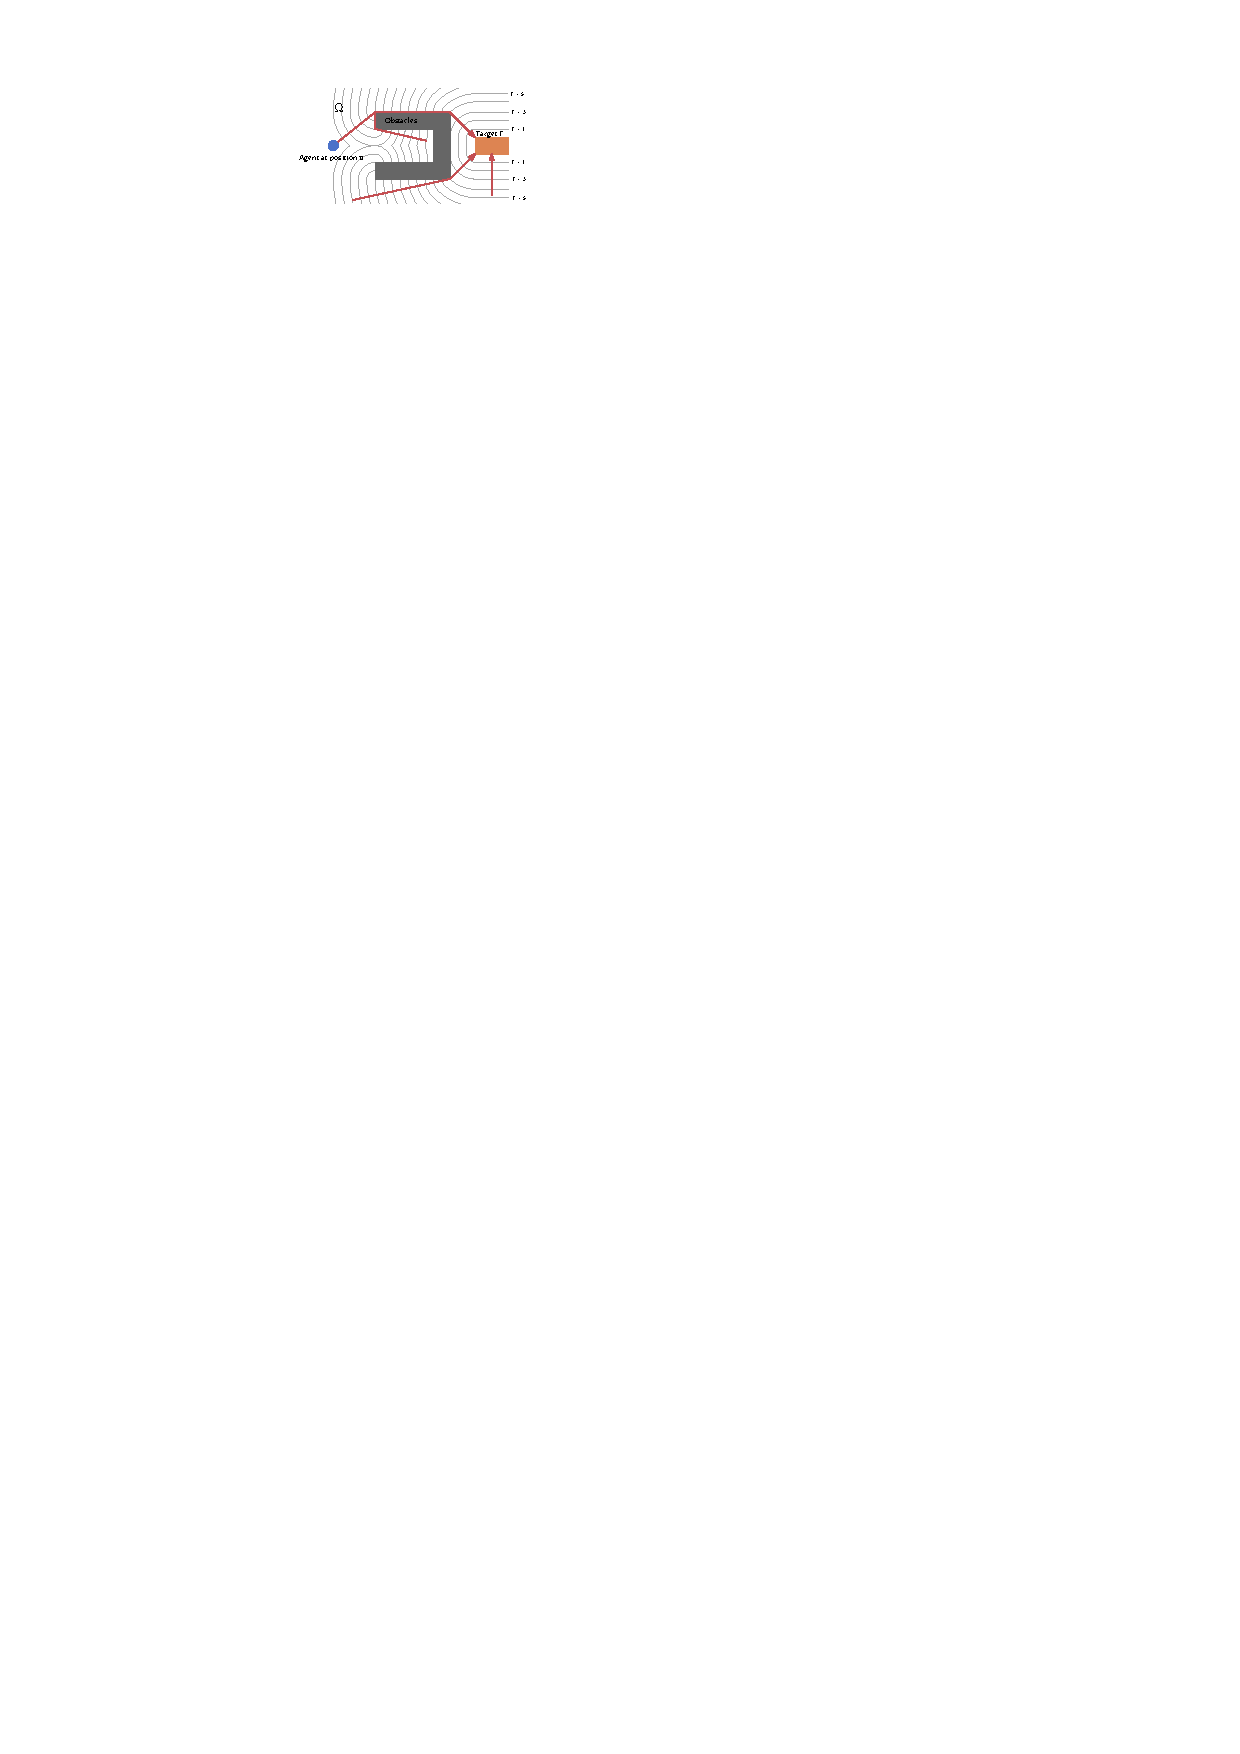
\includegraphics[width=0.6\textwidth]{./figs/chicken-eikonal_en.pdf}
	\end{figure}
	\uncover<3->{The change in travel time $T$ (over the space) is equal to $1/f$.}
\end{frame}

\begin{frame}
	\frametitle{The Eikonal Equation}
	\textbf{A one-dimensional case:} Let $\domain = [-1;1], \osmDestination = \{-1,1\}$.
	\begin{figure}
		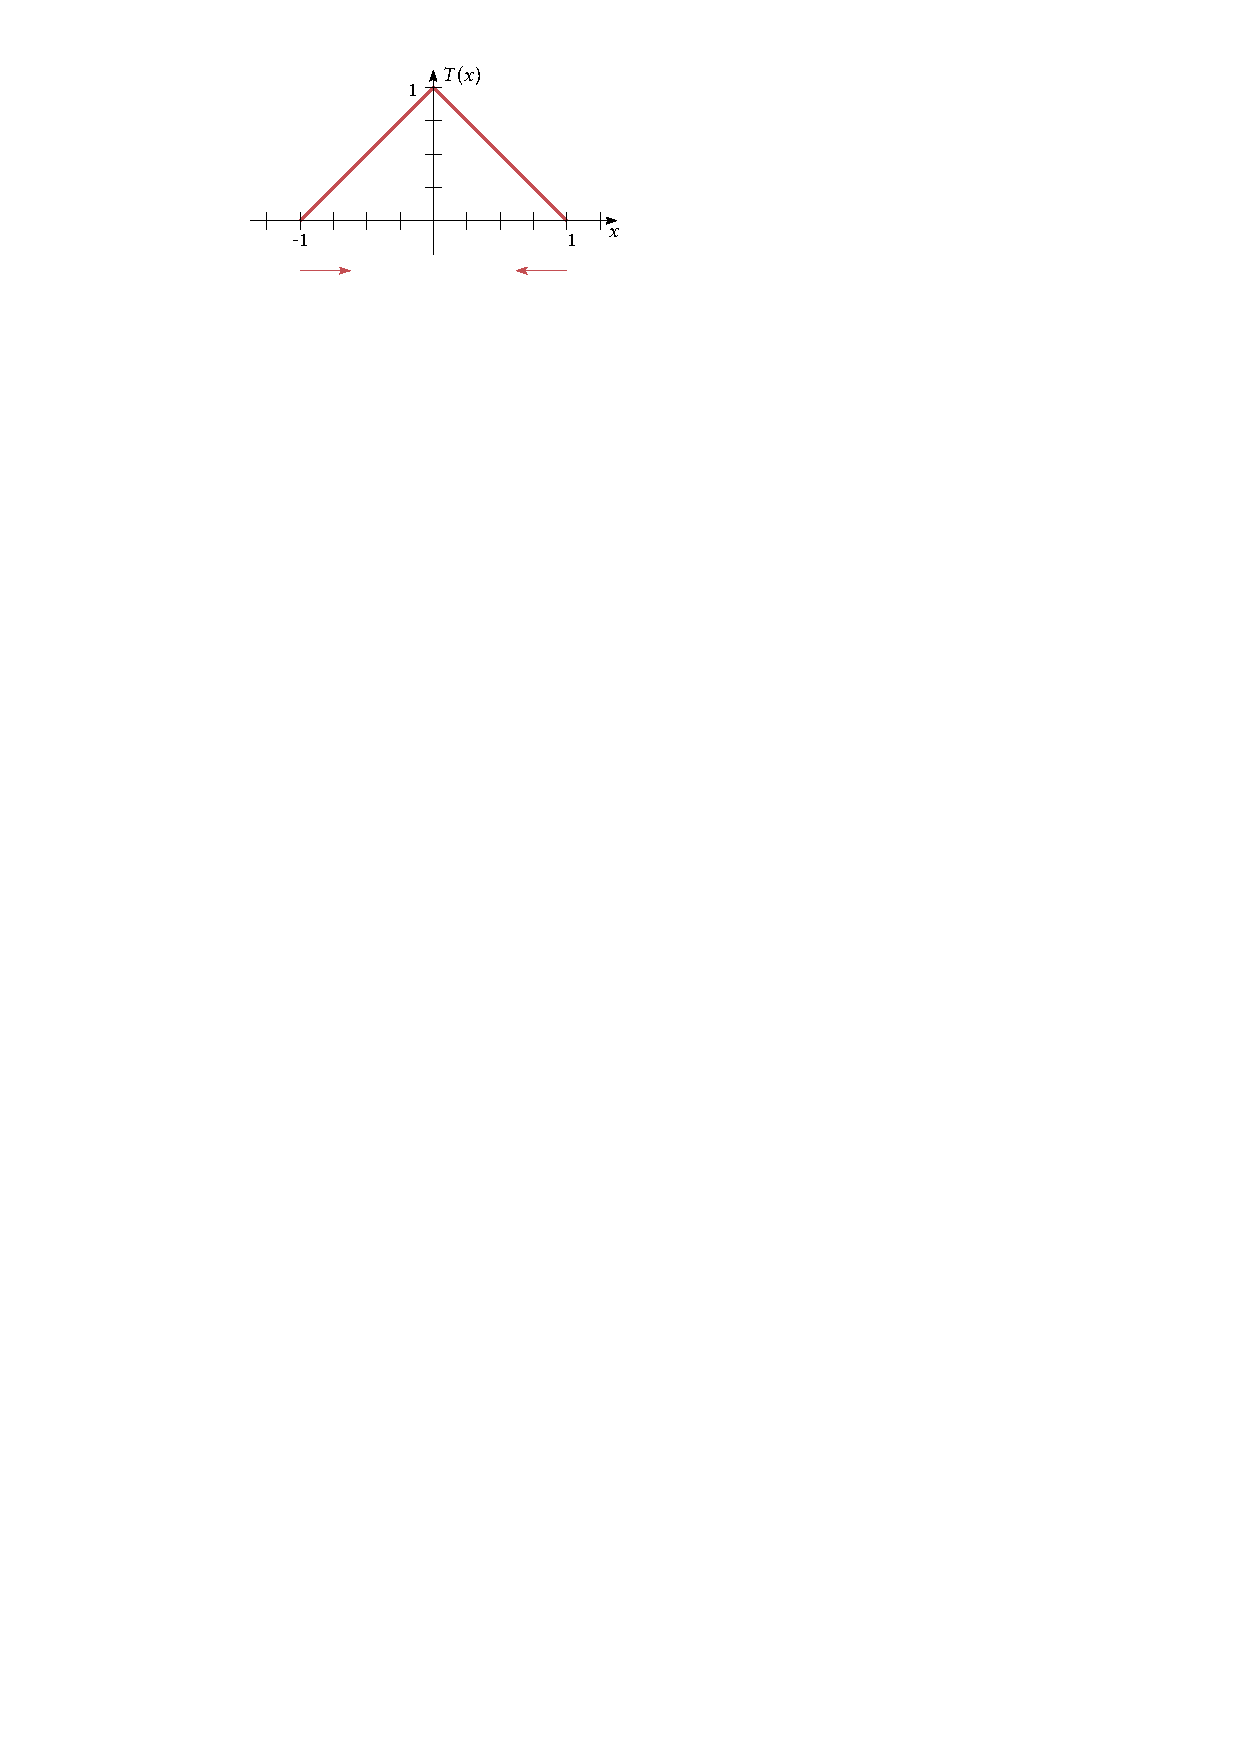
\includegraphics[width=0.6\textwidth]{./figs/1d-eikonal.pdf}
	\end{figure}
	\uncover<2->{$\Rightarrow T(x) = 1 - |x|$, is the viscosity solution of the \textbf{eikonal equation}!}
	
%	Im $\mathbb{R}$ ist dieser Sachverhalt leicht ersichtlich:
%	Stellen Sie sich vor Sie laufen (mit der Zeit $t$) auf einer Linie mit der Geschwindigkeit $f = 1$.
%	\begin{equation*}
%		\frac{dx}{dt} = df \Rightarrow \frac{dt}{dx} = \frac{1}{df}
%	\end{equation*}
%	\begin{center}
%			'Mit der \textbf{Reisegeschwindigkeit} $f$ von einem Meter pro Sekunde, laufen Sie in einer Sekunden einen Meter'.
%	\end{center}
\end{frame}


\begin{frame}
	\frametitle{The Eikonal Equation}
	We imagine a \textbf{wavefront} propagating with a \textbf{travel speed} $f(\uu) = 1$ from the target $\osmDestination$ across the region $\domain$.\\
	\vspace{0.25cm}
	
	$T(\uu)$ is the \textbf{travel time} or arrival time of the \textbf{wavefront} at the location $\uu$.
	
	\begin{figure}
		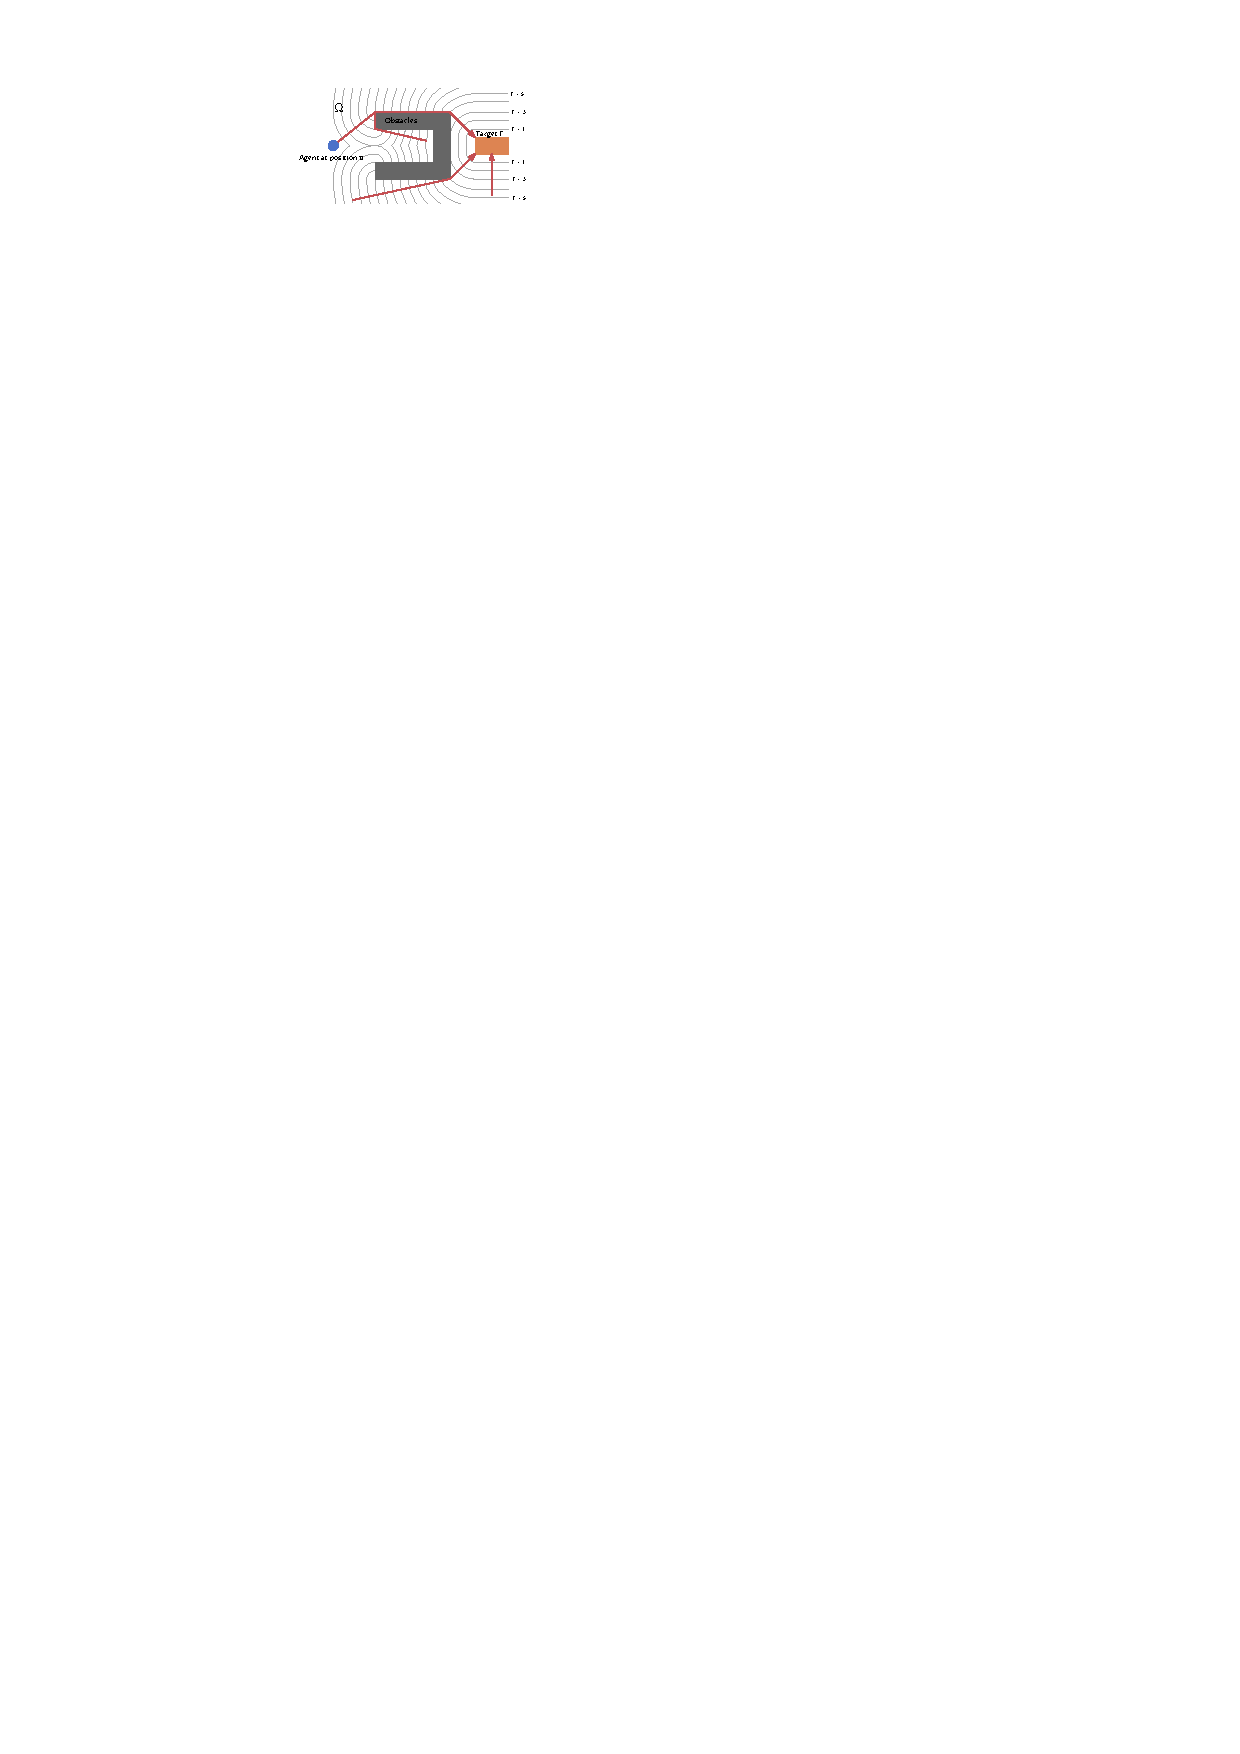
\includegraphics[width=0.6\textwidth]{./figs/chicken-eikonal_en.pdf}
	\end{figure}
	The change in travel time $T$ (over the space) is equal to $1/f$.
\end{frame}

\begin{frame}
	\frametitle{The Eikonal Equation}
	The \textbf{wavefront}, which propagates at \textbf{travel speed} $f(\uu) = 1$ from the target $\osmDestination$ over the domain $\domain$, can be described by the  \textbf{eikonal equation}:
	%\begin{block}{Solution of the eikonal equation}
	\uncover<2->{\begin{equation}
	\begin{split}
		\Vert \nabla T(\uu) \Vert \cdot f(\uu) &= 1, \, \uu \in \domain\\
		T(\uu) &= 0, \ \uu \in \osmDestination\\
		f(\uu) & \geq 0, \ \uu \in \domain.
	\end{split}
	\end{equation}}
\uncover<3->{\textbf{Remarks:}}
\begin{enumerate}[label=(\roman*)]
	\uncover<3->{\item It is a hyperbolic partial equation}
	\uncover<3->{\item Initial condition: $T(\uu) = 0 \text{ for } \uu \in \osmDestination$}
	\uncover<3->{\item For the viscosity solution $T$ does not has to be differential everywhere}
	\uncover<3->{\item If $f = 1$ holds, then is $T$ equal to the \textbf{geodesic distance}.}
\end{enumerate}
\end{frame}

\begin{frame}[plain]
	\begin{center}
		{\color{myblue} \huge The Fast Marching Method (FMM)}
	\end{center}
\end{frame}

\subsection{The Fast Marching Method}
\begin{frame}
	\frametitle{The Fast Marching Method}
	The \textsc{FastMarchingMethod} \cite{sethian-1999,kimmel-1998} computes a numerical solution of the eikonal equation on a discrete grid (or mesh). The algorithm imitates the propagation of the \textbf{wavefront}.\\
	\vspace{1cm}
	
	\uncover<2->{The method uses the same strategy compared to the \textsc{Dijkstra} but instead of computing distances between nodes it computes the \textbf{travel time} $T(\uu)$ of a wavefront that propagates over the space and not only over edges.}
\end{frame}

\begin{frame}
	\frametitle{The Fast Marching Method}
	During the comutation, each grid point is part of exactly one of the following sets:
	\begin{enumerate}[label=(\roman*)]
		\uncover<1->{\item \textit{far}: The wavefront is far away (white)}
		\uncover<1->{\item \textit{considered}: The wavefront is close (blue)}
		\uncover<1->{\item \textit{accepted}: The wavefront reached this point (black)}
	\end{enumerate}
	\begin{figure}
		\subfigure{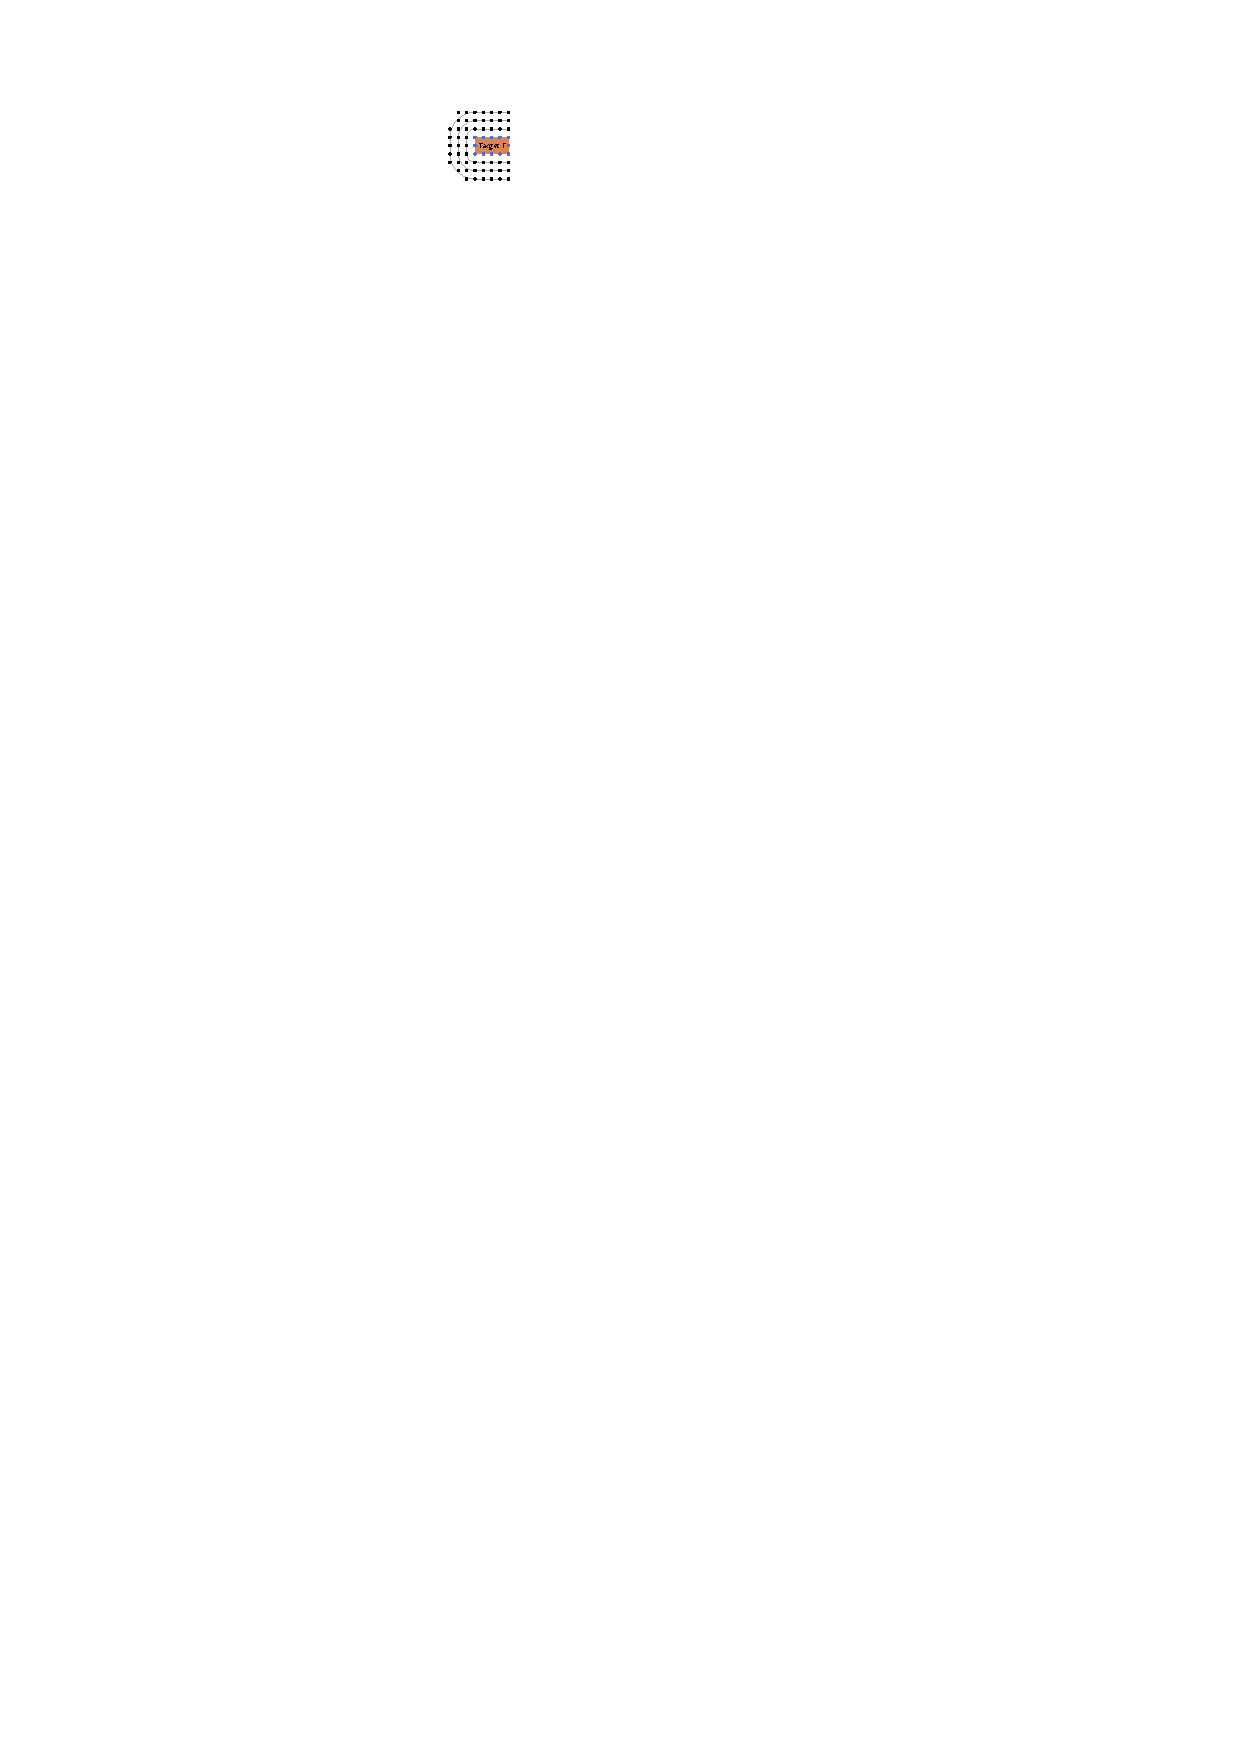
\includegraphics[width=0.23\textwidth]{./figs/chicken-fmm-1_en.pdf}}
		\hspace{1cm}
		\subfigure{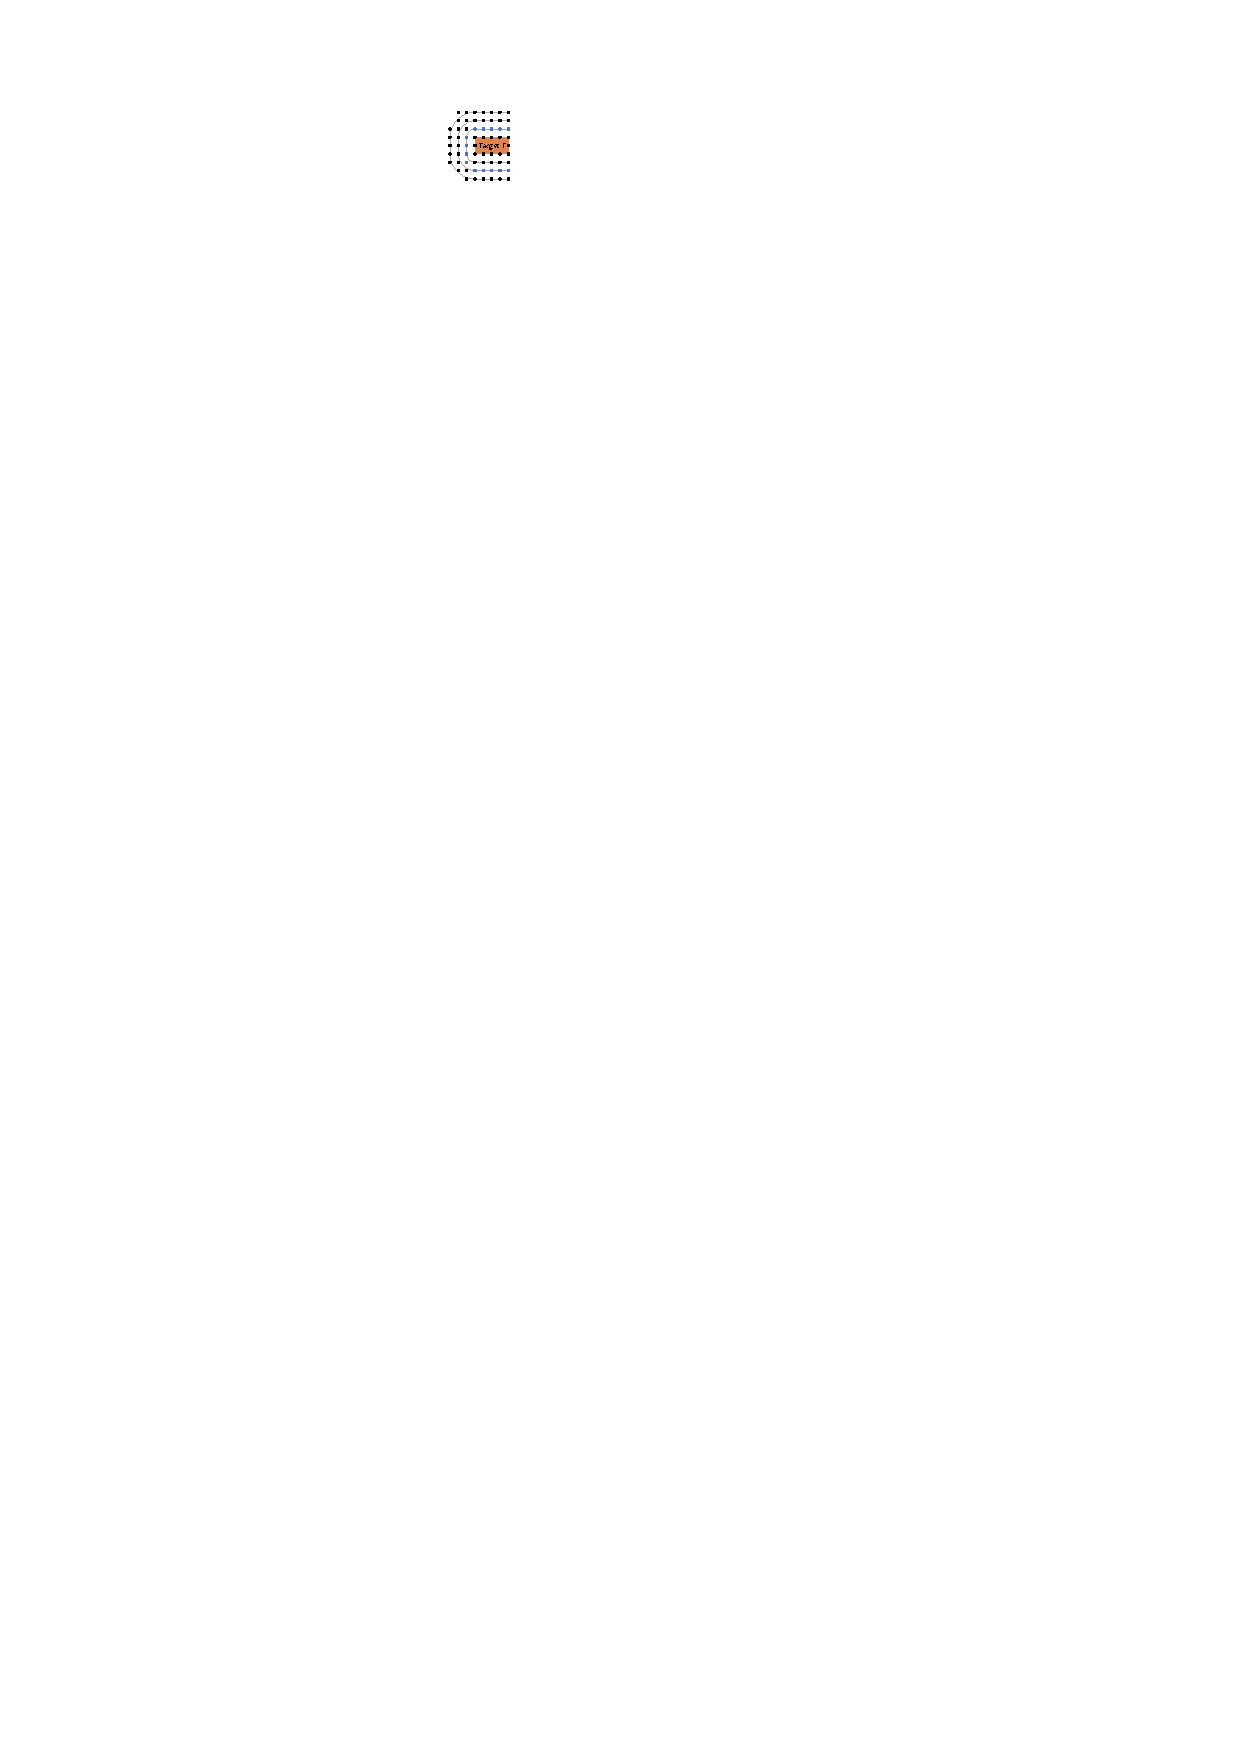
\includegraphics[width=0.23\textwidth]{./figs/chicken-fmm-2_en.pdf}}
		\hspace{1cm}
		\subfigure{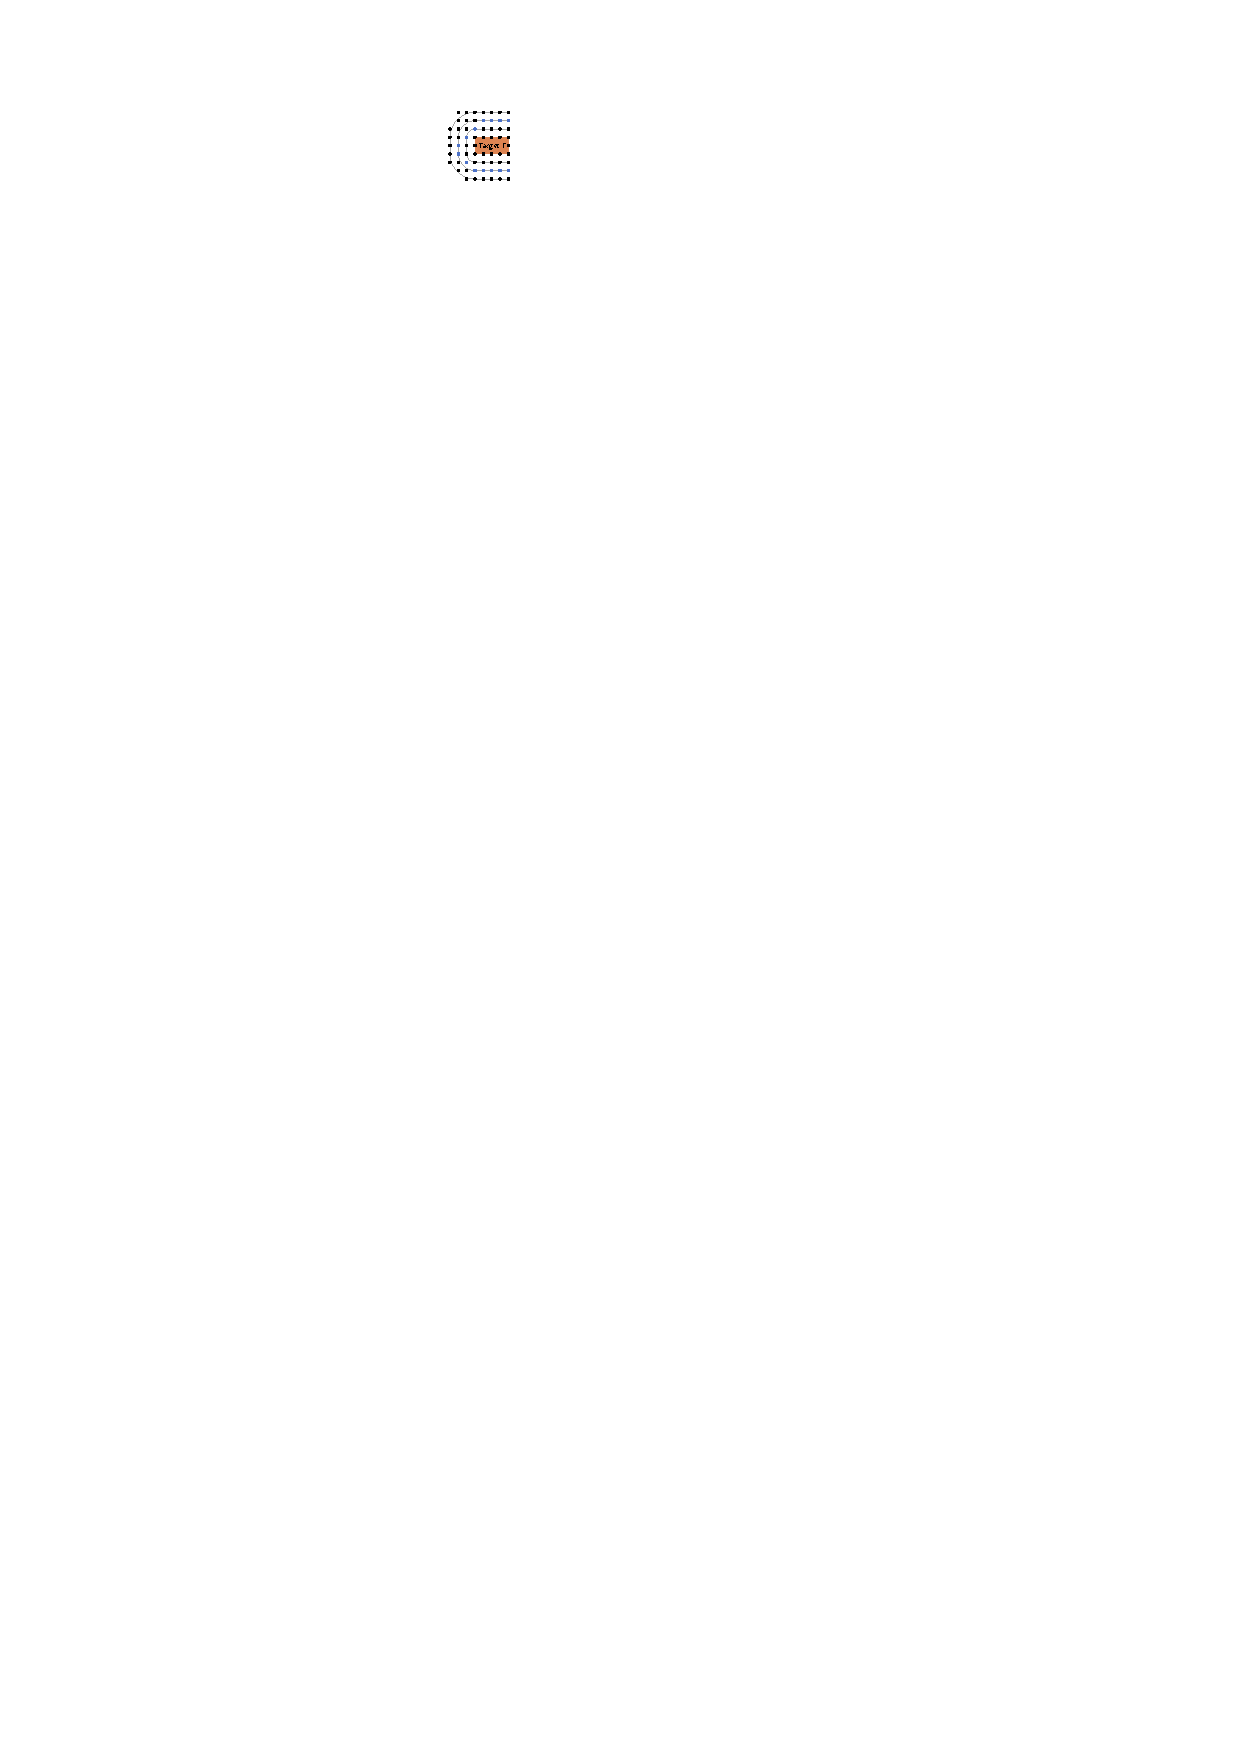
\includegraphics[width=0.23\textwidth]{./figs/chicken-fmm-3_en.pdf}}
	\end{figure}
\end{frame}

\begin{frame}
	\frametitle{Solving the Eikonal Equation}
	The \textbf{wavefront} reaches every grid point $\uu_{i,j}$ by coming from a certain direction (within one of the four quadrants):
	\begin{figure}
		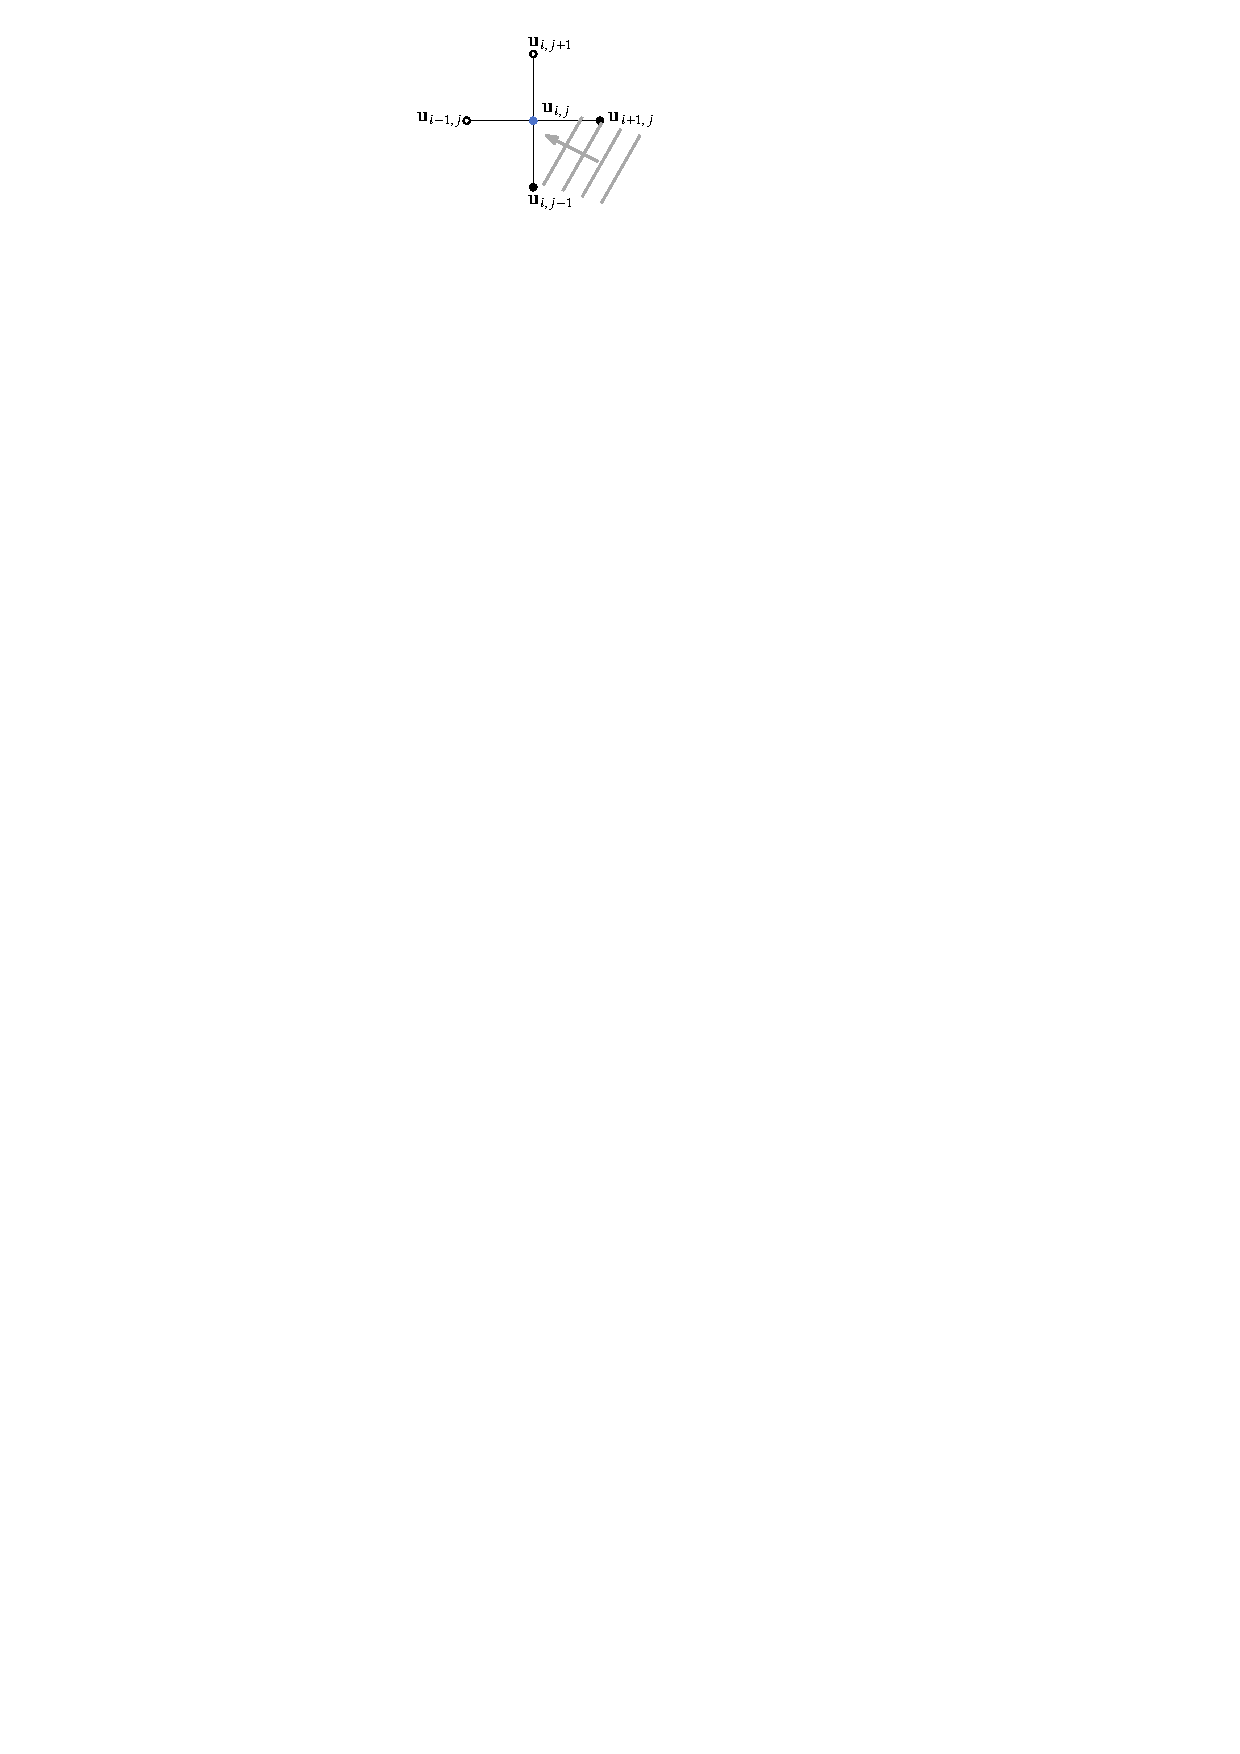
\includegraphics[width=0.5\textwidth]{./figs/stencil.pdf}
	\end{figure}
	Based on the stancil of we compute the \textbf{travel time} $T(\uu_{i,j})$.
\end{frame}

\begin{frame}
	\frametitle{Solving the Eikonal Equation}
	%	\begin{equation}
	%		\Vert \nabla T(\xx)\Vert^2 = f(\mathbf{x})^{-2},
	%	\end{equation}	
	We can approximate $\nabla T$ by a finite difference (Taylor-expansion):
	\begin{columns}
		\begin{column}{0.4\textwidth}
			\uncover<2->{\begin{equation*}
			\begin{split}
				\frac{\partial T(\uu_{i,j}) }{\partial x} &\approx D^{\pm x}_{i,j}\uu = \frac{
					T(\uu_{i \pm 1,j}) - {\color{myblue} T(\uu_{i,j})} }{\pm \Delta x}\\
				\frac{\partial T(\uu_{i,j})}{\partial y} &\approx D^{\pm y}_{i,j}\uu = \frac{
					T(\uu_{i,j \pm 1}) - {\color{myblue} T(\uu_{i,j})} }{\pm \Delta y}.
			\end{split}
		\end{equation*}}
		\end{column}
		\begin{column}{0.45\textwidth}
				\begin{figure}
				\centering
				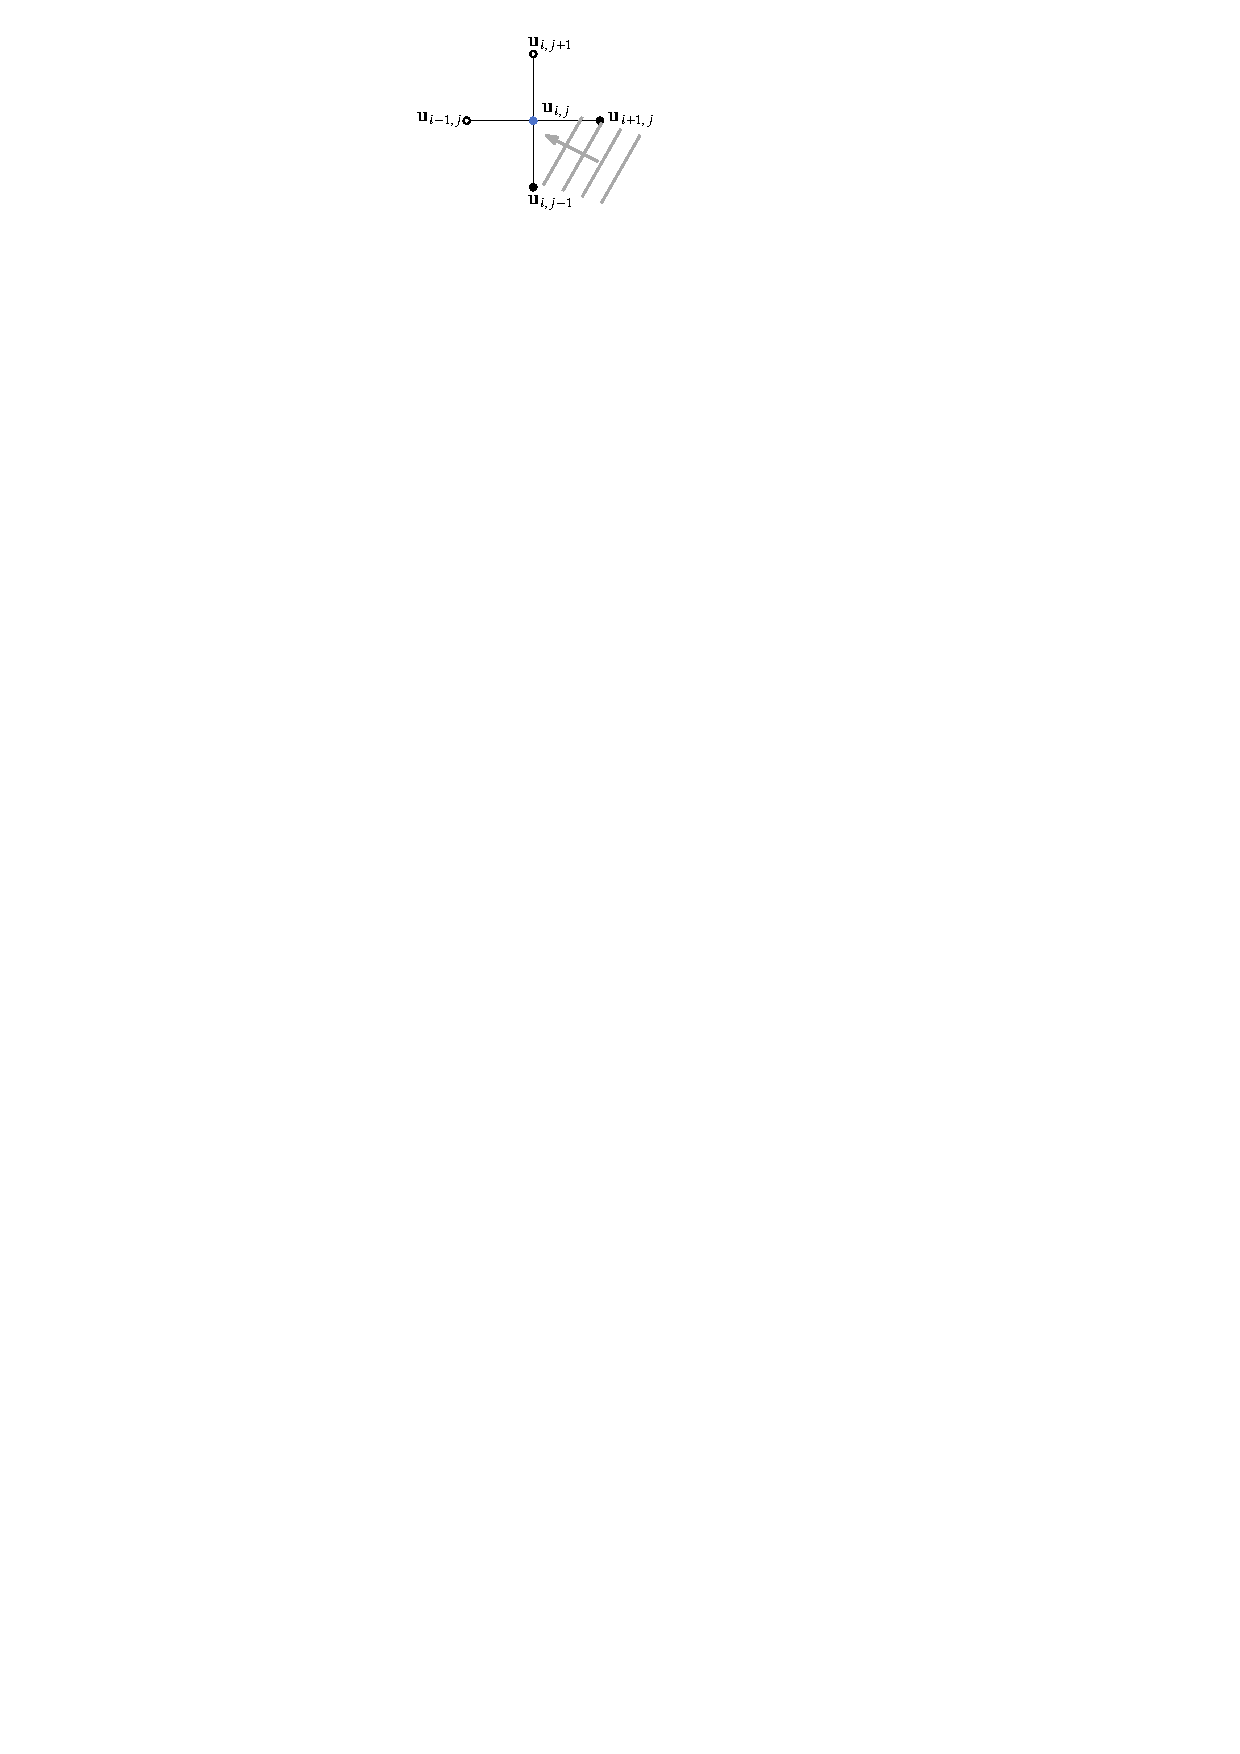
\includegraphics[width=0.8\textwidth]{./figs/stencil.pdf}
			\end{figure}
		\end{column}
	\end{columns}
	\vspace{0.5cm}
	\uncover<3->{If we knew that the wave arrives from right below, we only would require
	\begin{equation*}
		D^{+ x}_{i,j}\uu = \frac{
			T(\uu_{i + 1,j}) - { \color{myblue} T(\uu_{i,j})} }{+ \Delta x} \text{ und } D^{- y}_{i,j}\uu = \frac{
			T(\uu_{i,j - 1}) - {\color{myblue} T(\uu_{i,j})} }{- \Delta y}.
	\end{equation*}}
\end{frame}

\begin{frame}
	\frametitle{Solving the Eikonal Equation}
	How do we arrive at an expression for ${\color{myblue} T(\uu_{i,j})}$?
	\uncover<2->{\begin{equation}
		\Vert \nabla T(\uu) \Vert \cdot f(\uu) = 1
	\end{equation}}
	\uncover<3->{can be transformed to
	\begin{equation}
		\Vert \nabla T(\uu) \Vert^2 = \frac{1}{f(\uu)^2},
	\end{equation}}
	\uncover<4->{which can be further transformed into
	\begin{equation}
		(D^{+ x}_{i,j}\uu)^2 + (D^{- y}_{i,j}\uu)^2 = f(\uu_{i,j})^{-2}.
	\end{equation}
	(if we knew the wave arrives from right below). Therefore, we solve for ${\color{myblue} T(\uu_{i,j})}$ in the quadratic equation
	\begin{equation}
		\left( \frac{ T(\uu_{i + 1,j}) - { \color{myblue} T(\uu_{i,j})} }{+ \Delta x} \right)^2 + \left( \frac{
			T(\uu_{i,j - 1}) - {\color{myblue} T(\uu_{i,j})} }{- \Delta y} \right)^2 = f(\uu_{i,j})^{-2}.
	\end{equation}
	}
\end{frame}

\begin{frame}
	\frametitle{Solving the Eikonal Equation}
	The major difference to the the \textsc{Dijkstra} is the computation of the \textbf{travel time} $T(\uu)$.
	\begin{figure}
		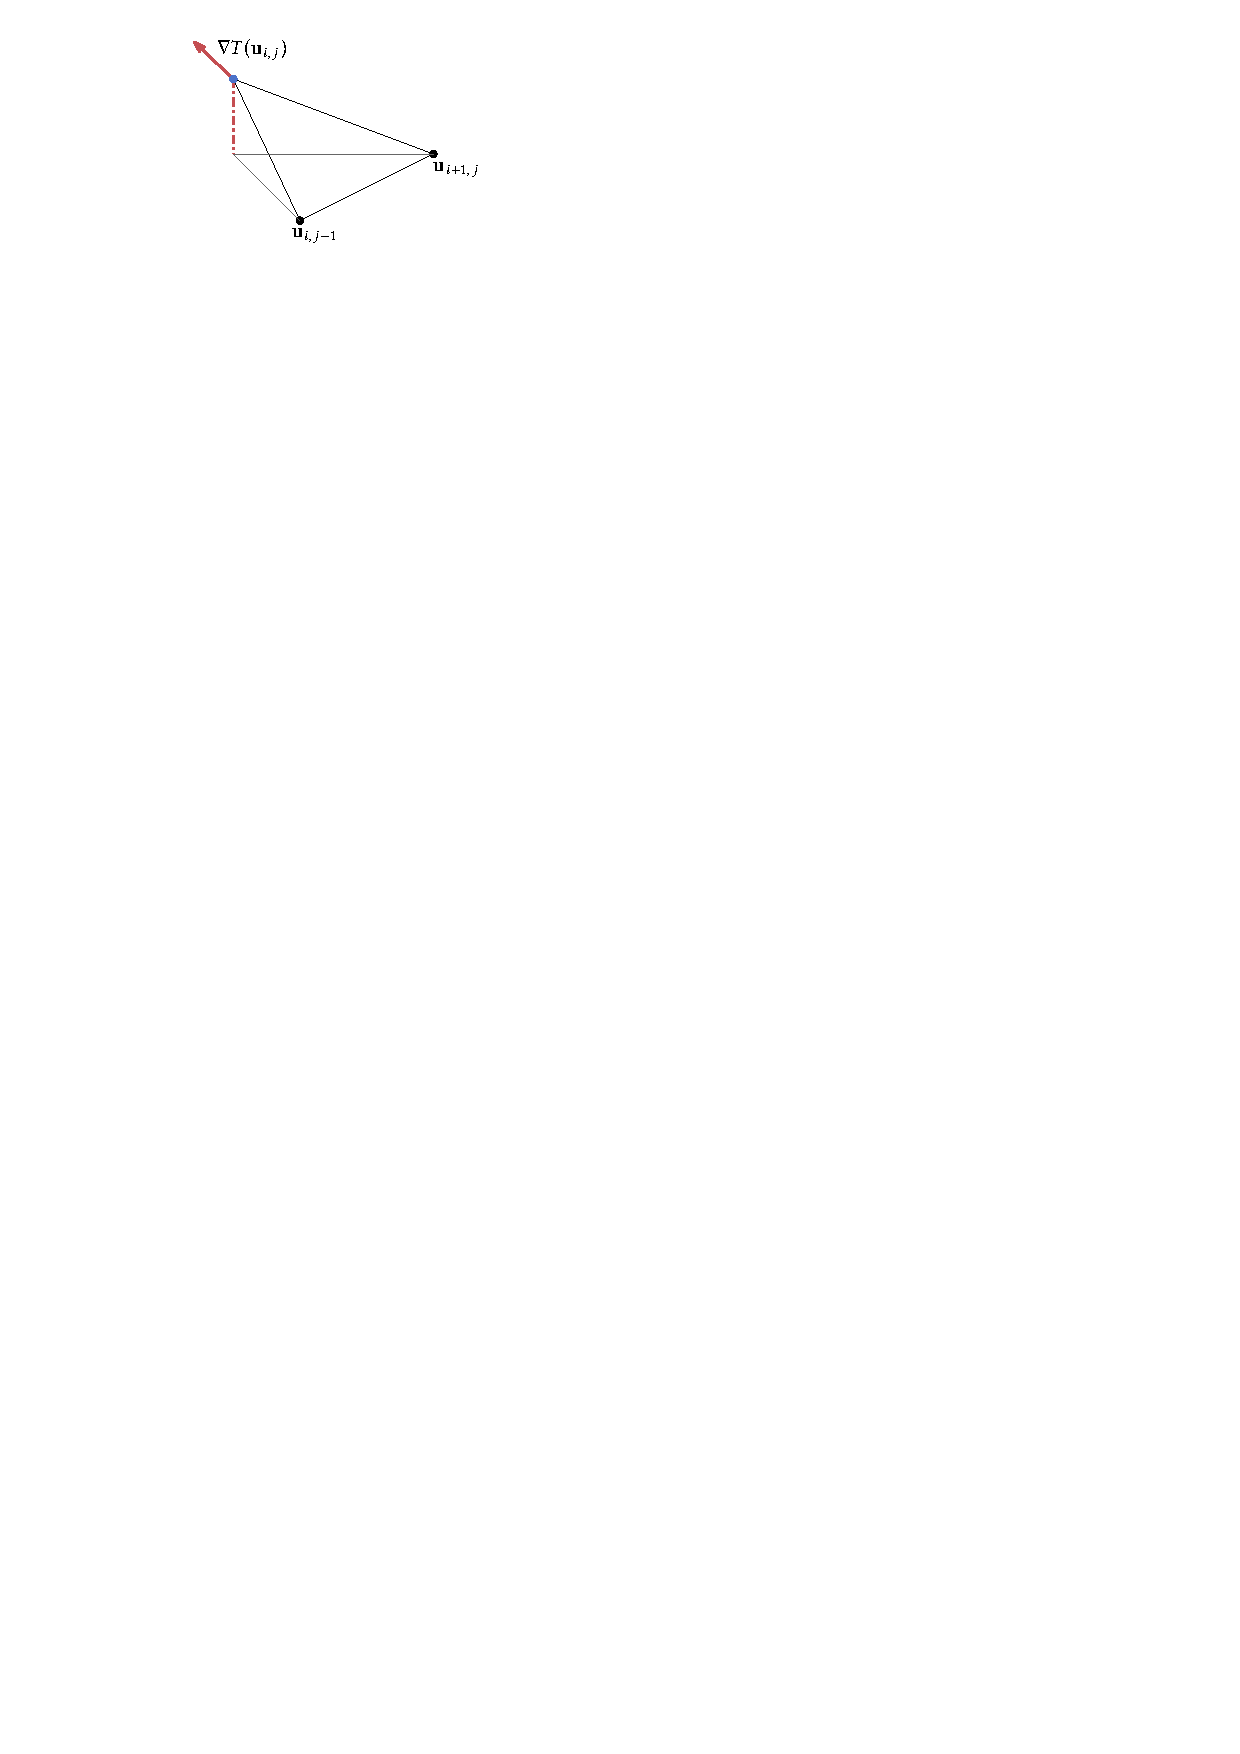
\includegraphics[width=0.6\textwidth]{./figs/eikonal-lokal.pdf}
	\end{figure}
\end{frame}

\begin{frame}
	\frametitle{Solving the Eikonal Equation}
	In general, we do not konw the direction from wich the wavefront arrives at $\uu_{i,j}$.
	\uncover<2->{In $x-$direction it arrives from either \textbf{left} or \textbf{right} AND in $y$-direction from either \textbf{above} or \textbf{below}.}\\
	\vspace{0.25cm}
	\uncover<3->{\textbf{Right, below:}
	\begin{equation*}
		\left( \frac{ T(\uu_{i + 1,j}) - { \color{myblue} T(\uu_{i,j})} }{+ \Delta x} \right)^2 + \left( \frac{
			T(\uu_{i,j - 1}) - {\color{myblue} T(\uu_{i,j})} }{- \Delta y} \right)^2 = f(\uu_{i,j})^{-2}
	\end{equation*}}

	\uncover<4->{\textbf{Left, above:}
	\begin{equation*}
		\left( \frac{ T(\uu_{i - 1,j}) - { \color{myblue} T(\uu_{i,j})} }{- \Delta x} \right)^2 + \left( \frac{
			T(\uu_{i,j + 1}) - {\color{myblue} T(\uu_{i,j})} }{+ \Delta y} \right)^2 = f(\uu_{i,j})^{-2}
	\end{equation*}}
	
	\uncover<5->{We assume that the wavefront arrives from the direction it arrives first.}
\end{frame}

\begin{frame}
	\frametitle{Solving the Eikonal Equation}
	We assume that the \textbf{wavefront} arrives from the direction from which it arrives first at $\uu_{i,j}$.\\
	\vspace{0.5cm}
	\uncover<2->{Therefore,
	\begin{equation*}
		(D^{+ x}_{i,j}\uu)^2 + (D^{- y}_{i,j}\uu)^2 = f(\uu_{i,j})^{-2}
	\end{equation*}}
	\uncover<3->{can be transformed into
	\begin{equation} \label{eq:local:eikonal:2}
		\max\left\{ D_{i,j}^{-x}\uu, -D_{i,j}^{+x}\uu \right\}^2 + \max\left\{ D_{i,j}^{-y}\uu, -D_{i,j}^{+y}\uu \right\}^2 = f(\uu_{i,j})^{-2}.
	\end{equation}
	We solve this eqaution locally using Godunov's scheme \cite{kimmel-1998,sethian-2000}.}
\end{frame}

\begin{frame}
	\frametitle{Solving the Eikonal Equation}
	%	\begin{equation}
	%		\Vert \nabla T(\xx)\Vert^2 = f(\mathbf{x})^{-2},
	%	\end{equation}	
	We could use a more accurate approximation of $\nabla T$ useing an additional Taylor-terms. 
	\uncover<2->{Remember:
	\begin{equation}
			f(x + h) \approx f(x) + h f'(x)  + h^2\frac{f''(x)}{2} \Rightarrow 
		f'(x) \approx \frac{f(x + h) - f(x)}{h} - \frac{h}{2}f''(x)
	\end{equation}}
	\uncover<3->{For our approximation of the differentiation
	\begin{equation}
		D^{\pm x}_{i,j}\uu = \frac{T(\uu_{i \pm 1,j}) - {\color{myblue} T(\uu_{i,j})} }{\pm \Delta x}
	\end{equation}
	we get
	\begin{equation}
		(D^{\pm x}_{i,j})'\uu \approx \frac{T(\uu_{i \pm 2,j}) - 2T(\uu_{i \pm 2,j}) + {\color{myblue} T(\uu_{i,j})} }{\pm (\Delta x)^2}.
	\end{equation}}
	\uncover<4->{Therefore
	\begin{equation*}
			\frac{\partial T(\uu_{i,j}) }{\partial x} \approx D^{\pm 2x}_{i,j}\uu = \frac{
			T(\uu_{i \pm 1,j}) - {\color{myblue} T(\uu_{i,j})} }{\pm \Delta x} - \frac{\Delta x}{2} \frac{T(\uu_{i \pm 2,j})-2 T(\uu_{i \pm 1,j}) + {\color{myblue} T(\uu_{i,j})} }{\pm (\Delta x)^2}
	\end{equation*}}
\end{frame}

\begin{frame}
	\frametitle{Solving the Eikonal Equation}
	Therefore
	\begin{equation*}
		\begin{split}
		\frac{\partial T(\uu_{i,j}) }{\partial x} \approx D^{\pm 2x}_{i,j}\uu &= \frac{
			T(\uu_{i \pm 1,j}) - {\color{myblue} T(\uu_{i,j})} }{\pm \Delta x} - \frac{\Delta x}{2} \frac{T(\uu_{i \pm 2,j})-2 T(\uu_{i \pm 1,j}) + {\color{myblue} T(\uu_{i,j})} }{\pm (\Delta x)^2} \\
		&=  \frac{2T(\uu_{i \pm 1,j}) - {\color{myblue} 2T(\uu_{i,j})} }{\pm 2\Delta x} - \frac{T(\uu_{i \pm 2,j})-2 T(\uu_{i \pm 1,j}) + {\color{myblue} T(\uu_{i,j})} }{\pm 2 \Delta x} \\
		&=  \frac{-T(\uu_{i \pm 2,j}) + 4 T(\uu_{i \pm 1,j}) - 3{\color{myblue} T(\uu_{i,j})} }{\pm 2 \Delta x}.
		\end{split}
	\end{equation*}
	The same can be computed for the$y$-direction:
	\begin{equation*}
		\frac{\partial T(\uu_{i,j}) }{\partial y} \approx D^{\pm 2y}_{i,j}\uu =  \frac{- T(\uu_{i,j\pm 2}) + 4 T(\uu_{i,j\pm 1}) - 3{\color{myblue} T(\uu_{i,j})} }{\pm 2 \Delta y}.
	\end{equation*}
\end{frame}

\begin{frame}
	\frametitle{Solving the Eikonal Equation}
	We still solve a quadratic equation:
	\begin{equation} \label{eq:lokal:eikonal:1}
		\max\left\{ D_{i,j}^{-2x}\uu, -D_{i,j}^{+2x}\uu \right\}^2 + \max\left\{D_{i,j}^{-2y}\uu, -D_{i,j}^{+2y}\uu \right\}^2 = f(\uu_{i,j})^{-2}.
	\end{equation}\\
	\vspace{0.5cm}
	\uncover<2->{\textbf{Advantage:} A better rate of convergence for with respect to the grid resolution ($\Delta x, \Delta y \rightarrow 0$), since 
	\begin{equation*}
		f(x + h) = f(x) + h f'(x) + \alert{\mathcal{O}(h^2)} = f(x) + h f'(x) + h^2\frac{f''(x)}{2} + \alert{\mathcal{O}(h^3)}
	\end{equation*}\\}
	\vspace{0.5cm}
	\uncover<3->{\textbf{Disadvantage:} Possible unintended smoothing of singularities.}
\end{frame}

\begin{frame}[fragile]
	\frametitle{The Fast Marching Method}
	\begin{algorithm}[H]
		%\KwIn{triangulation $\mesh$, spatial destination $\osmDestination$, spatial domain $\domain$}
		%\KwOut{$\eikonalApp_\osmDestination$ solution of \cref{eq:eikonal:repeat}}
		
		$T_\uu \leftarrow \infty$ for all $\uu \in \domain$\;
		$T_\uu  \leftarrow 0$ for all $\uu \in \osmDestination$\;
		$\mathcal{B} \leftarrow \emptyset$ \tcp{reached points}
		
		$\mathcal{Q} \leftarrow \left\{ (\uu, T_\uu) \mid \uu \in \osmDestination \right\}$ \tcp{considered points}
		%	\ForEach{$\vvv \in \osmDestination$}{
		%		$\mathcal{H} \leftarrow \mathcal{H} \cup (\vvv, \eikonal_\osmDestination(\vvv))$\;
		%	}
		\While{$\mathcal{Q} \neq \emptyset$}{ \label{alg:navi:fmm:while}
			$(\uu, T_\uu) \leftarrow \mathcal{Q}.\textsc{pop}()$\;
			\ForEach{neighbor $\vvv$ of $\uu$ with $\vvv \not\in \mathcal{B}$}{
				$T_\vvv  \leftarrow$ \textsc{SolveEikonal}($\vvv$)\;
				\eIf{$(\vvv, T_\vvv) \in \mathcal{Q}$}{
					$\mathcal{Q}.\textsc{decrease}(\vvv, T_\vvv)$\;
				}
				{
					$\mathcal{Q}.\textsc{push}(\vvv, T_\vvv)$\;
				}
			}
			%$\mathcal{Q} \leftarrow \mathcal{Q} \setminus \{(\uu, T(\uu))\}$\;
			$\mathcal{B} \leftarrow \mathcal{B} \cup \{ \uu \}$\;
		}
		$T \leftarrow \left\{ (\uu, T_\uu) \right\}$\;
		\textbf{return} $T$\;
		%\caption{\textsc{FastMarchingMethod}} \label{alg:navi:fmm}
	\end{algorithm}
\end{frame}

\begin{frame}
	\frametitle{The Fast Marching Method}
	$\mathcal{Q}$ is a \textsc{PriorityQueue} sorted according to {\color{myblue}$T_\uu$}
	\begin{enumerate}[label=$\bullet$]
		\item $\mathcal{Q}.\textsc{pop}()$, returns the point with the smalles arrival time,
		\item $\mathcal{Q}.\textsc{decrease}(\uu, T_\uu)$ changes the element, 
		\item and $\mathcal{Q}.\textsc{push}(\uu, T_\uu)$ adds an element
		\item \textsc{SolveEikonal}($\uu$) solves lokal solution of \cref{eq:lokal:eikonal:1} or \cref{eq:local:eikonal:2}.
	\end{enumerate}
	\vspace{0.5cm}
	\uncover<2->{\textbf{Complexity:} (for $n$ nodes)
	\begin{enumerate}[label=$\bullet$]
		\item Time: $\mathcal{O}(n\log(n))$
		\item Memory: $\mathcal{O}(n)$
	\end{enumerate}}
\end{frame}

\begin{frame}
	\frametitle{The Fast Marching Method}
	\textbf{Hints for your implementation:}
	\begin{enumerate}[label=$\bullet$]
		\uncover<2->{\item You find a good description in \cite{baerentzen-2001}.}
		\uncover<3->{\item To quickly check whether a grid point is \textit{far}, \textit{considered}, or \textit{reached}, use a \textbf{flag} (not a set).}
		\uncover<4->{\item You can also initialize points around $\osmDestination$ with, for example, the value of the Euclidean distance and insert them into $\mathcal{Q}$.}
		\uncover<5->{\item You can gain some performance by skipping $\textsc{decrease}$ and using only $\textsc{push}$ (i.e., allowing duplicate entries $\Rightarrow$ you need to adjust the algorithm slightly, see \cite{jones-2006})}
	\end{enumerate}
\end{frame}

\begin{frame}
	\frametitle{The Fast Marching Method}
	\textbf{Properties:}
	\begin{enumerate}[label=$\bullet$]
		\item[+] Very fast sequential algorithm for all types of waves
		\item[+] Especially fast for 'narrow' waves
		\uncover<2->{\item[-] Difficult to parallelize, attempts \cite{herrmann-2003,yang-2015}
			\item[-] Requires complicated/unstructured \textsc{PriorityQueue}
			\item[-] Does not exploit the parallelism of wavefront propagation}
	\end{enumerate}
	\vspace{0.25cm}
	\uncover<3->{\textbf{Alternative methods:}
		\begin{enumerate}[label=$\bullet$]
			\item \textsc{FastSweepingMethod} \cite{zhao-2005}, suitable only for very 'simple' waves
			\item \textsc{FastIterativeMethod} \cite{jeong-2008}, particularly suitable for 'broad' waves
			\item \textsc{InformedFastIterativeMethod} (my dissertation), suitable for repeated calculations of slightly changing waves.
	\end{enumerate}}
	\uncover<4->{In \cite{capozzoli-2013,gomez-2015} you can find comparisons of different methods.}
\end{frame}

\begin{frame}[plain]
	\begin{center}
		{\color{myblue} \huge Modelling using the Traveling Speed Function}
	\end{center}
\end{frame}

\subsection{Modelling using the Traveling Speed Function}
\begin{frame}
	\frametitle{Modelling using the Traveling Speed Function}
	How do we ensure that agents do not walk directly along the walls?\\
	\begin{figure}
		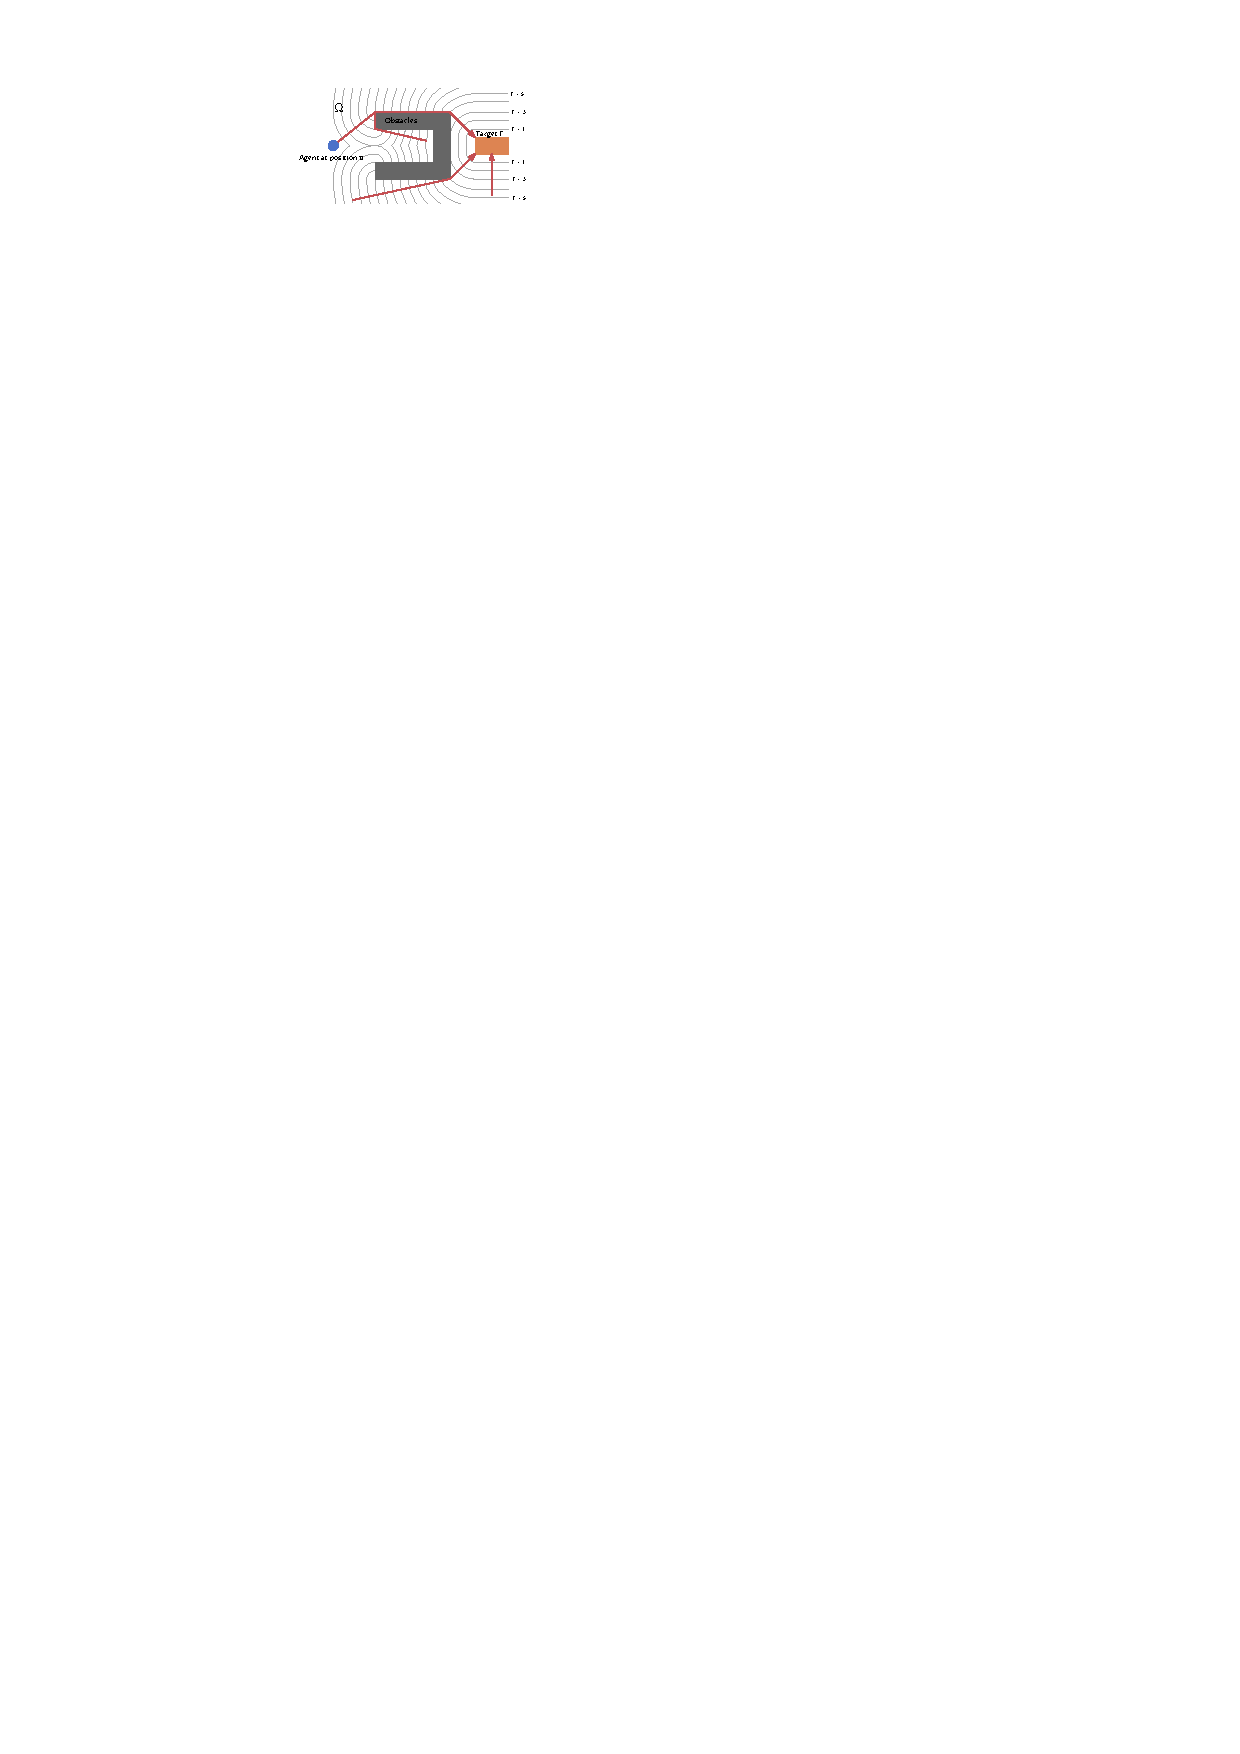
\includegraphics[width=0.6\textwidth]{./figs/chicken-eikonal_en.pdf}
	\end{figure}
	\uncover<2->{\textbf{Tip:} Reduce the travel speed of the wave $f$ near obstacles!}
\end{frame}

\begin{frame}
	\frametitle{Modelling using the Traveling Speed Function}
	For example, let $d_W(\uu)$ be the Euclidean distance to the nearest obstacle/wall, then
	\begin{equation*}
		f(\uu) = \begin{cases}
			1 / (2-(d_W(\uu)/ \delta_{W})) & \quad \text{if } d_W(\uu) < \delta_{W} \\
			1  & \quad \text{otherwise}.
		\end{cases}
	\end{equation*}
	might be suitable.
	\begin{figure}
		\subfigure[$\delta_{W} = 0.2$ meters]{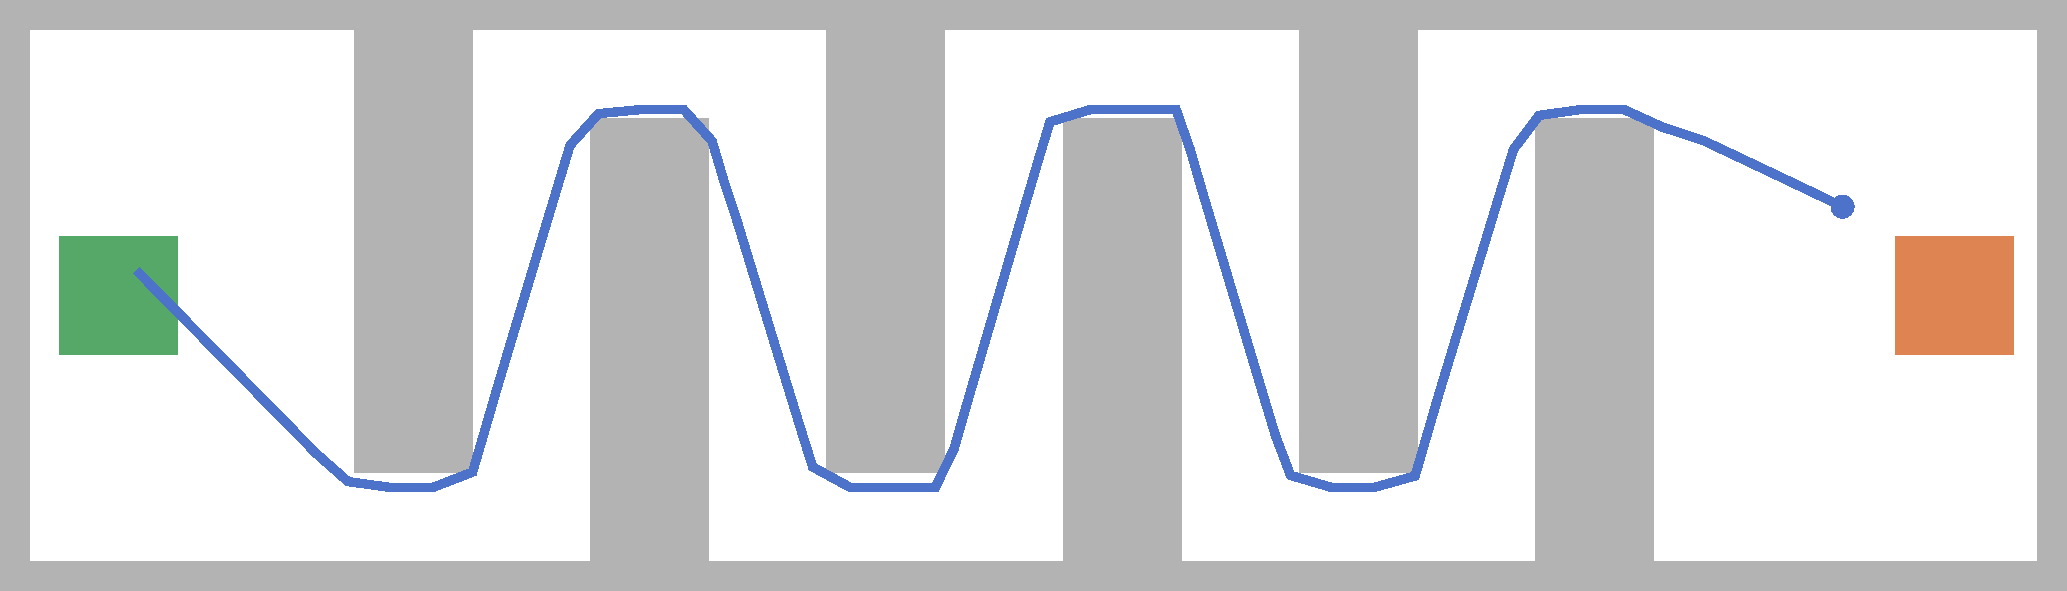
\includegraphics[width=0.38\textwidth]{./figs/bhm_0_2.pdf}}
		\hfill
		\subfigure[$\delta_{W} = 0.5$ meters]{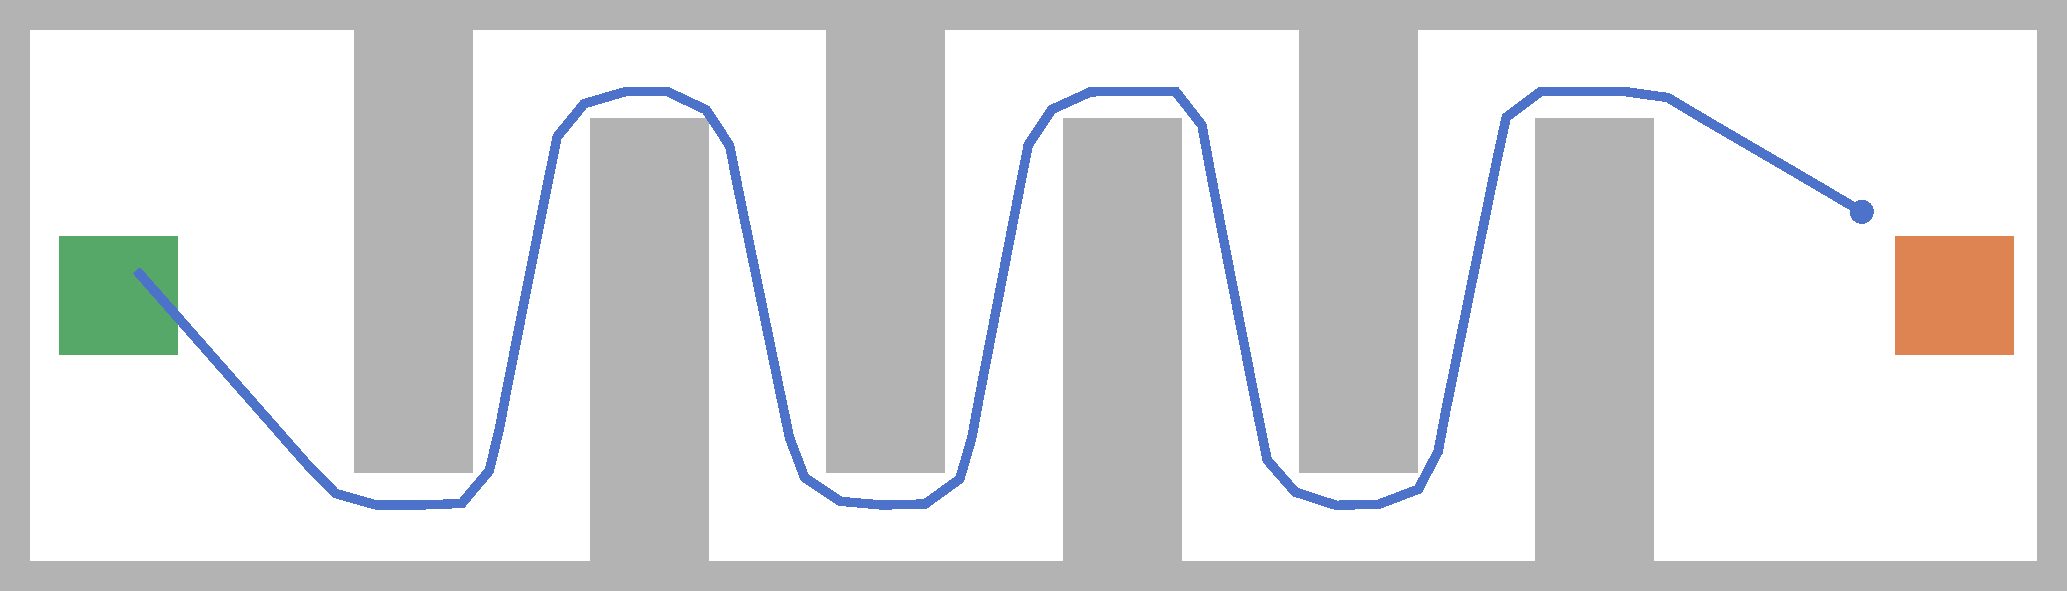
\includegraphics[width=0.38\textwidth]{./figs/bhm_0_5.pdf}}
		\hfill
		\subfigure[$\delta_{W} = 1.0$ meters]{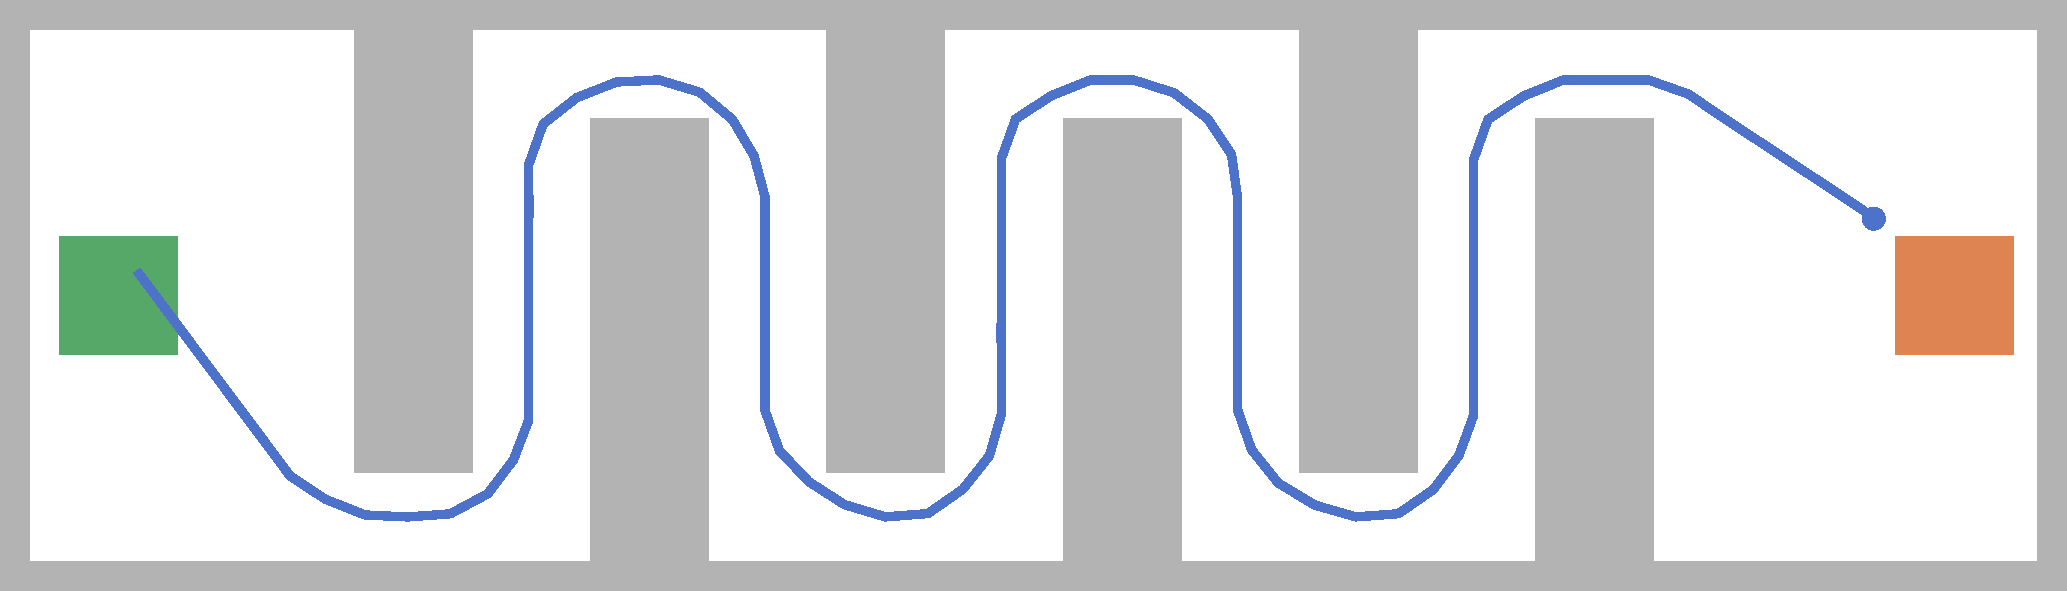
\includegraphics[width=0.38\textwidth]{./figs/bhm_1_0.pdf}}
	\end{figure}
\end{frame}


\begin{frame}
	\frametitle{Modelling using the Traveling Speed Function}
	\vspace{-0.5cm}
	\begin{figure}
		\subfigure[$T(\uu)$ for $f(\uu) = 1$]{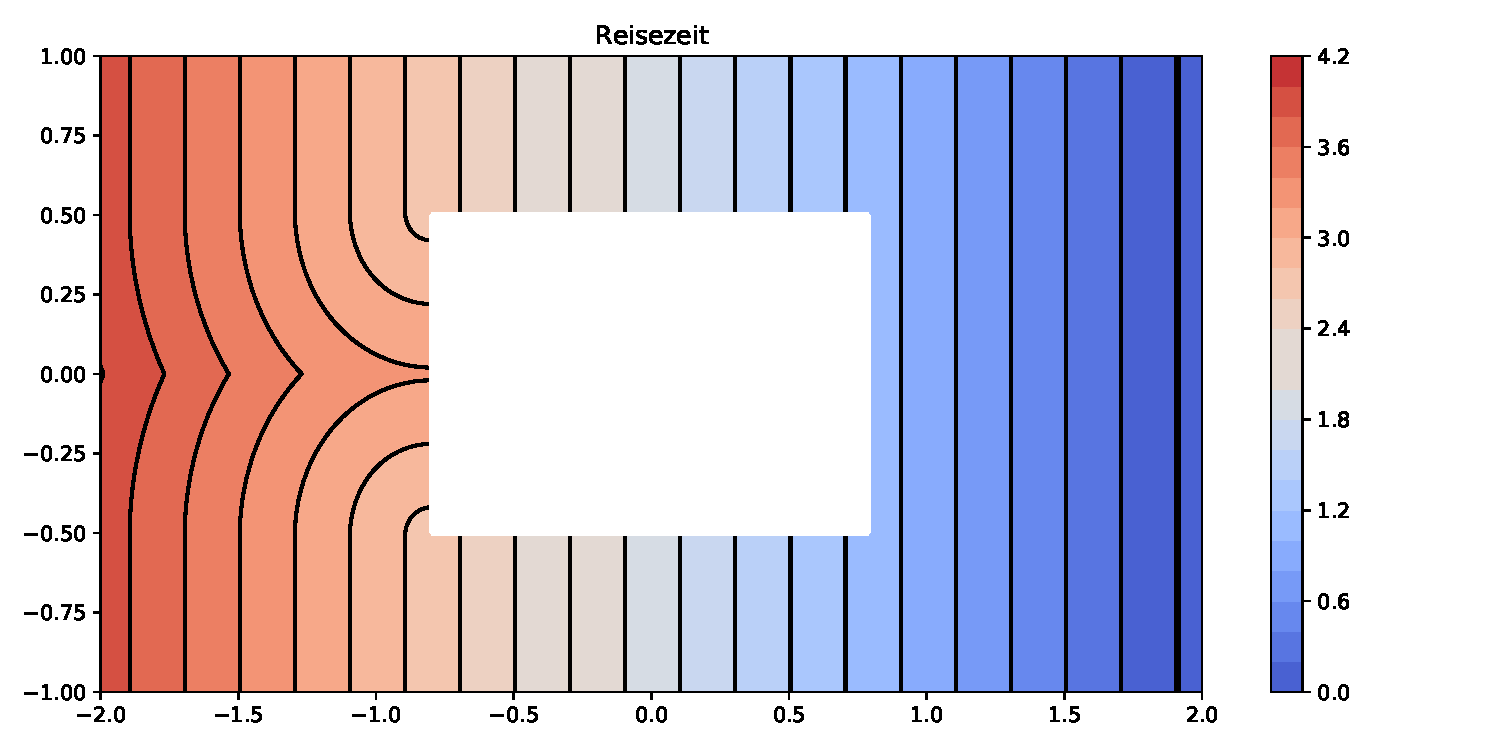
\includegraphics[width=0.43\textwidth]{./figs/reisezeit-hindernis.pdf}}\\
		\subfigure[$T(\uu)$ for $f(\uu) \leq 1$]{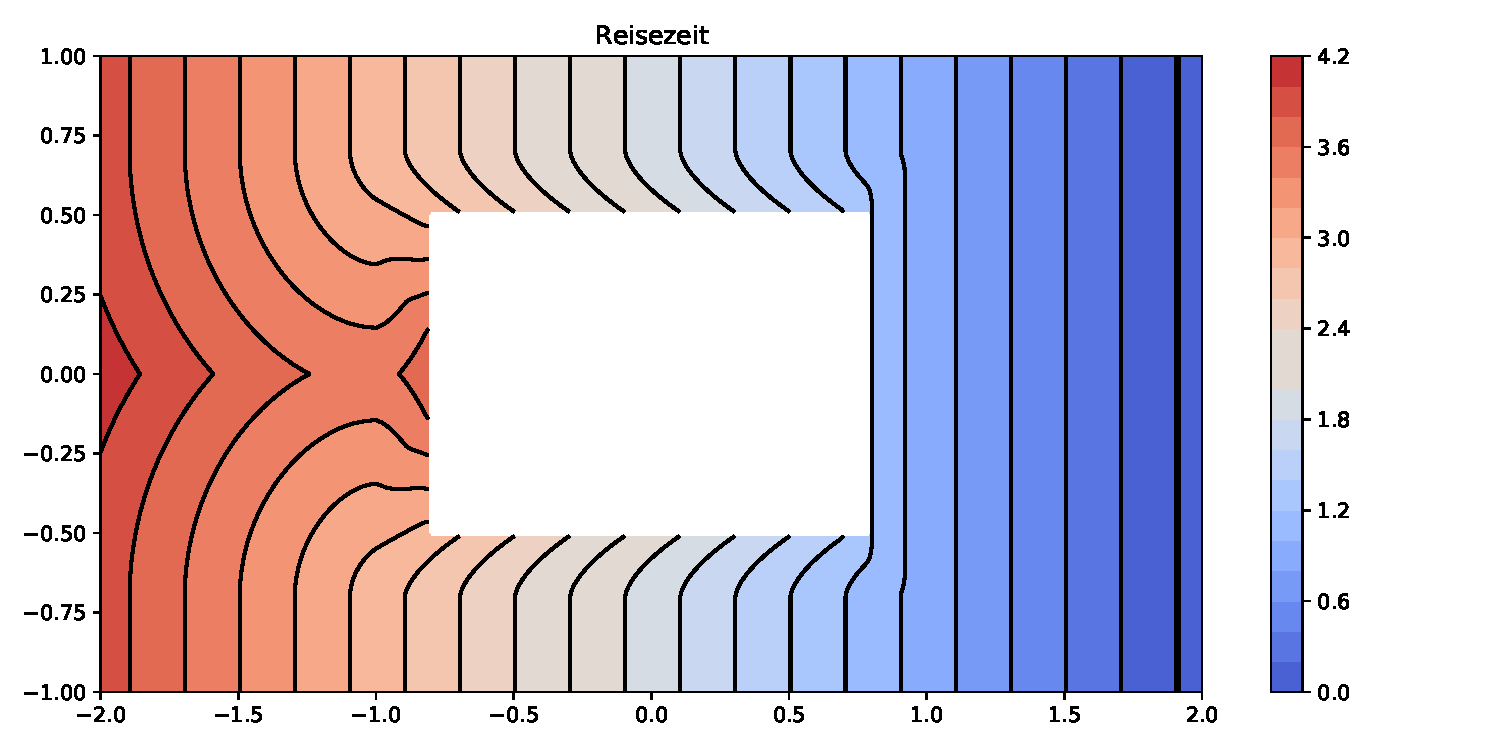
\includegraphics[width=0.43\textwidth]{./figs/reisezeit-hindernis-verlangsamung.pdf}}
		\hfill
		\subfigure[$f(\uu) \leq 1$]{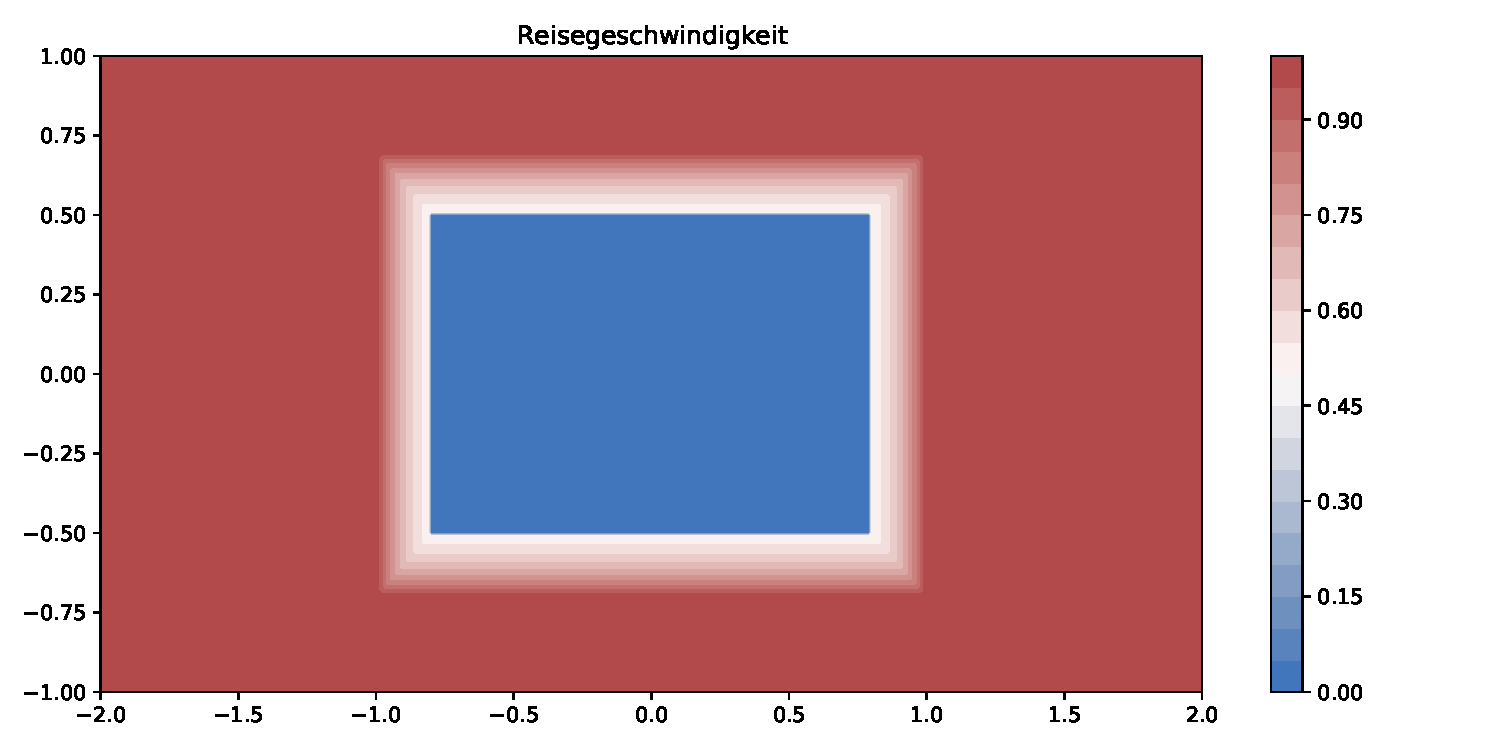
\includegraphics[width=0.43\textwidth]{./figs/reisegeschwindigkeit-hindernis-verlangsamung.pdf}}
	\end{figure}
\end{frame}

%\begin{frame}
%	\frametitle{Modelling using the Traveling Speed Function}
%
%\end{frame}
%
%\begin{frame}
%	\frametitle{Modelling using the Traveling Speed Function}
%	
%\end{frame}

\begin{frame}[allowframebreaks]
	\frametitle{References}
	{\scriptsize% dirty fix for the non-chapter bib
		\bibliographystyle{plainnat}
		\bibliography{Literature,Lit}}
\end{frame}

\end{document}
